% if you don't want two-sided printing, erase the twoside option
% from the following line:
\documentclass[12pt]{report}

% custom file for BSU style by KvW, 2006:
\usepackage{BSUthesis}

\usepackage{amssymb}
\usepackage{nomencl}
\makenomenclature

%% This code creates the groups
% -----------------------------------------
\usepackage{etoolbox}
\renewcommand\nomgroup[1]{%
  \item[\bfseries
  \ifstrequal{#1}{S}{Symbols}{%
  \ifstrequal{#1}{A}{Abbreviations}{%
  \ifstrequal{#1}{O}{Other symbols}{}}}%
]}
% -----------------------------------------

% \usepackage{acro}
% probably a good idea for the nomenclature entries:
% \acsetup{first-style=short}
\usepackage{siunitx}
\usepackage{wrapfig}
\usepackage{listings}
\usepackage[utf8]{inputenc}
\usepackage{geometry}


\newcommand\inputfile[1]{%
    \InputIfFileExists{#1}{}{\typeout{No file #1.}}%
} % this command keep latexmk from erroring when \input is missing

\newcommand{\todo}[1]{\textcolor{red}{#1 -- TODO}}
\newcommand{\ej}[1]{\textcolor{red}{EJ: #1}}
%\newcommand\tab[1][1cm]{\hspace*{#1}}
% For abbreviations
% For symbols and nomenclature 
\makenomenclature
%\usepackage{amssymb}
%\usepackage{nomencl}
%\makenomenclature

\nomenclature[S]{\(F[n]\)}{Electron density functional}
\nomenclature[S]{\(n(\textbf{r})\)}{Electron density}
\nomenclature[S]{T}{Temperature}
\nomenclature[S]{E}{Energy}
\nomenclature[S]{$\Delta E$}{Energy Difference}
\nomenclature[S]{\(E_{v}[n]\)}{Ground state energy}
\nomenclature[S]{\(E_{known}\)}{Kinetic, potential, and hartree energy}
\nomenclature[S]{\(E_{XC}\)}{Exchange-correlation energy}
\nomenclature[S]{$E[{\Psi_{i}}]$}{Total energy of the system}
\nomenclature[S]{\(v(\textbf{r})\) }{External potential}
\nomenclature[S]{\(F[n(\textbf{r})]\)}{Density functional that is independent of the external potential}
\nomenclature[S]{\(U_{LJ}(r_{ij})\)}{Potential energy of two particles (\(i,j\))}
\nomenclature[S]{\(r_{ij}\)}{Internuclear distance of two particles (\(i,j\)}
\nomenclature[S]{$\sigma$}{Van der Waals radius}
\nomenclature[S]{$\epsilon$}{Depth of the Lennard-Jones potential well}
\nomenclature[S]{$r$}{Bond distance}
\nomenclature[S]{$r_0$}{Equilibrium bond distance}
\nomenclature[S]{$\theta$}{Bond angle}
\nomenclature[S]{$\theta_0$}{Equilibrium bond angle}
\nomenclature[S]{$k_h$}{Harmonic bond constant}
\nomenclature[S]{$k_{\theta}$}{Harmonic angle constant}
\nomenclature[S]{U}{Potential energy}
\nomenclature[S]{$k_n$}{Spring constant of particle n}
\nomenclature[S]{$\phi$}{Dihedral angle}
\nomenclature[S]{cm\textsuperscript{-1}}{Inverse centimeters}
\nomenclature[S]{K}{Kelvin}
\nomenclature[S]{N}{Number of particles}
\nomenclature[S]{N\textsubscript{monomers}}{Number of repeating units in a polymer}
\nomenclature[S]{V}{Volume}
\nomenclature[S]{$d\mu/dQ$}{Dipole moment derivative}
\nomenclature[S]{a,b,c, $\beta$}{Unit Cell Parameters}
\nomenclature[S]{I}{Scattering intensity}
\nomenclature[S]{A}{Particle size distribution scalar}
\nomenclature[S]{b}{Exponential factor }
\nomenclature[S]{$\upsilon$}{Frequency}
\nomenclature[S]{\AA}{Angstrom}
\nomenclature[S]{\AA\textsuperscript{-1}}{Inverse angstroms}
\nomenclature[S]{°}{Degrees}
\nomenclature[S]{kJ}{Kilojoules}
\nomenclature[S]{s}{Seconds}
\nomenclature[S]{M}{Mass}
\nomenclature[S]{g/mL}{Grams per mililiter}
\nomenclature[S]{amu}{Atomic mass unit}
\nomenclature[S]{dt}{MD simulation timestep length}
\nomenclature[S]{$\langle R^2 \rangle$}{Mean squared end-to-end distance}
\nomenclature[S]{$\sqrt{\langle R^2 \rangle}$}{Root mean squared end-to-end distance}
\nomenclature[S]{$N_b$}{Number of bonds in a polymer}
\nomenclature[S]{$l_p$}{Persistence length}
\nomenclature[S]{$l_p^{MD}$}{Persistence length calculated via molecular dynamics}
\nomenclature[S]{$l_p^{SANS}$}{Persistence length calculated via small angle neutron scattering}
\nomenclature[S]{$l_p^{DFT}$}{Persistence length calculated via density functional theory}
\nomenclature[S]{$l_b$}{Average bond length}


\nomenclature[A]{MD}{Molecular Dynamics}
\nomenclature[A]{DFT}{Density Functional Theory}
\nomenclature[A]{BTDAH}{Barbituric Acid Dihydrate}
\nomenclature[A]{VAMH}{Violuric Acid Monohydrate}
\nomenclature[A]{OPV}{Organic Photovoltaic}
\nomenclature[A]{PCE}{Power conversion efficiency}
\nomenclature[A]{LDA}{Local density approximation} 
\nomenclature[A]{GGA}{generalized gradient approximation}
\nomenclature[A]{PV}{Photovoltaic}
\nomenclature[A]{LUMO}{Lowest unoccupied molecular orbital}
\nomenclature[A]{HOMO}{Highest occupied molecular orbital}
\nomenclature[A]{BHJ}{Bulk heterojunction}
\nomenclature[A]{LJ}{Lennard-Jones}
\nomenclature[A]{GAFF}{Generalized amber force field}
\nomenclature[A]{CPDT}{Cyclopentadithiophene}
\nomenclature[A]{PT}{Pyridalthiadiazole}
\nomenclature[A]{FBT}{Fluorobenzothiadiazole}
\nomenclature[A]{BT}{Benzothiadiazole}
\nomenclature[A]{IDT}{Indacenodithiophene}
\nomenclature[A]{PCPDTPT}{Cyclopentadithiophene-co-pyridalthiadiazole}
\nomenclature[A]{PCPDTFBT}{Cyclopentadithiophene-co-fluorobenzothiadiazole}
\nomenclature[A]{PIDTBT}{Indacenodithiophene-co-benzothiadiazole }
\nomenclature[A]{PIDTFBT}{Indacenodithiophene-co-fluorobenzothiadiazole}
\nomenclature[A]{PIDTCPDT}{Indacenodithiophene-co-cyclopentadithiophene}
\nomenclature[A]{PTFE}{Polytetrafluoroethylene}
\nomenclature[A]{BTA}{Barbituric acid}
\nomenclature[A]{THz}{Terahertz}
\nomenclature[A]{UA}{United atom}
\nomenclature[A]{OPLS}{Optimized Potentials for Liquid Simulations}
\nomenclature[A]{OPLS-UA}{United Atom Optimized Potentials for Liquid Simulations}
\nomenclature[A]{GAFF}{General amber force field}
\nomenclature[A]{ESP-UA}{United atom espaloma force field}
\nomenclature[A]{FWHM}{Full width half mass}
\nomenclature[A]{GIXS}{Grazing incident x-ray scattering}
\nomenclature[A]{SANS}{Small angle neutron scattering}
\nomenclature[A]{RDF}{Radial distribution factor}
\nomenclature[A]{CG}{Coarse Grain}
\nomenclature[A]{TPS}{Time steps per second}
\nomenclature[A]{P3HT}{Poly-3-hexylthiophene}
\nomenclature[A]{GHG}{Green-house gas}
\nomenclature[A]{GPU}{Graphical processing unit}
\makeglossaries

\newcommand{\esp}{\texttt{Espaloma}} 
\newcommand{\espff}{\texttt{ESP-UA}} 
\newcommand{\oplsff}{\texttt{OPLS-UA}} 

\begin{document}

%------------------------------------------------------------------------------
% bunch of fields to enter:
%------------------------------------------------------------------------------
\author{Madilyn E. Paul}
%------------------------------------------------------------------------------
%\degree{Doctor of Philosophy}
\degreetype{Doctor of Philosophy}
%------------------------------------------------------------------------------
\discipline{Materials Science and Engineering}
%------------------------------------------------------------------------------
\title{Development and application of computational tools for organic molecular structure prediction from small molecule crystal structure determination to polymer persistence length.} % use correct capitalization
%------------------------------------------------------------------------------
\advisor{Eric Jankowski}{Ph.D.}
\committeeMemberA{Scott Phillips}{Ph.D.}
\committeeMemberB{Oliviero Andreussi}{Ph.D.}
\committeeMemberC{Frank Willmore}{Ph.D.} 
%------------------------------------------------------------------------------
\dean{Scott Lowe}{Dean of the Graduate College}
%------------------------------------------------------------------------------
% insert month and year of your thesis, only:
\date{November 2024}
\oralexamdate{November 21, 2024}
%------------------------------------------------------------------------------
%------------------------------------------------------------------------------
\maketitle
%------------------------------------------------------------------------------
\makecopyright
%------------------------------------------------------------------------------
\submittalsheet
%------------------------------------------------------------------------------
\setcounter{page}{4}
\input dedication
%------------------------------------------------------------------------------
\input acknowledgment
%------------------------------------------------------------------------------
%\input autobiographics
%------------------------------------------------------------------------------
\input abstract
%------------------------------------------------------------------------------
% \cleardoublepage
\tableofcontents
%------------------------------------------------------------------------------
\cleardoublepage
\addcontentsline{toc}{chapter}{List of tables} 
\listoftables
%------------------------------------------------------------------------------
\cleardoublepage
\addcontentsline{toc}{chapter}{List of figures} 
\listoffigures
%------------------------------------------------------------------------------
% print abbreviations
%\printglossary[title={List of abbreviations},type=\acronymtype]
%------------------------------------------------------------------------------
% print symbols
\cleardoublepage% or \clearpage
%\renewcommand{\nomname}{List of Abbreviations}
%\markboth{\nomname}{\nomname}% maybe with \MakeUppercase
%%
\printnomenclature

%------------------------------------------------------------------------------
% start of main text (reset pagenumbers, etc.):
%------------------------------------------------------------------------------
\begintext

%------------------------------------------------------------------------------

\chapter{Introduction}
\label{chap:Intro}
\section{Polymorphism}
Polymorphism is the ability of a molecular solid, composed of the same molecular moieties, to exist in two or more crystalline conformations. These crystal conformations are called polymorphs and will transition from one to another under specific conditions, \autoref{polymorph_fig}. When polymorphism was first reported in 1832 by Friedrich Wçhler and Justus von Liebig, it was believed to affect only large, flexible molecules, such as proteins. However, as studies continued, it was discovered that over 50\% of molecules experience polymorphism \citep{cruz-cabeza_facts_2015,Hoja}.

\begin{figure}[ht]
    \centering
    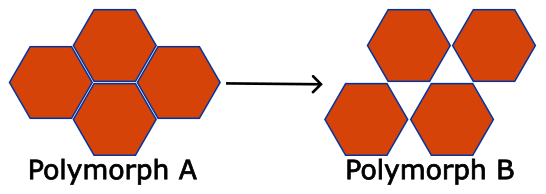
\includegraphics[width=12cm]{src/figures/intro_figs/polymorphism_fig.png}
    \caption{Diagram of a polymorphic phase transition from Polymorph A to Polymorph B.}
    \label{polymorph_fig}
\end{figure}

Due to the abundance of polymorphs and the influence of their crystalline structure on the intermolecular interactions present in a material, polymorphs and solvatomorph have become a widely growing area of study in fields of pharmaceutical development, crystal engineering, and de-novo materials design. Solvatomorphs are a specific class of polymorphs in which the solvent molecules crystallize with the solute molecules, see \autoref{solvatomorph_fig}. The system's intermolecular interactions are responsible for many of the substance’s properties, and can cause differences in solubility, vibrational spectra, densities, dissolution rate, melting point, mechanical properties, etc between crystal motifs \citep{Brittain2016,bernstein_polymorphism_2011,gentili_polymorphism_2019, Hoja}. Particularly difficult to characterize, hydrates are also a commonly observed branch of crystalline materials. Hydrates are a class of solvatomorphs in which at least one water molecule crystallizes within the unit cell with the solute molecules. These water molecules make studying polymorphism particularly difficult because of the extra degree(s) of freedom the molecules have when crystallizing and transitioning between polymorphs. In this study, we discuss our investigation of the possible polymorphism of barbituric acid dihydrate (BTADH) and violuric acid monohydrate (VAMH) using density functional theory (DFT). 
\begin{figure}[ht]
    \centering
    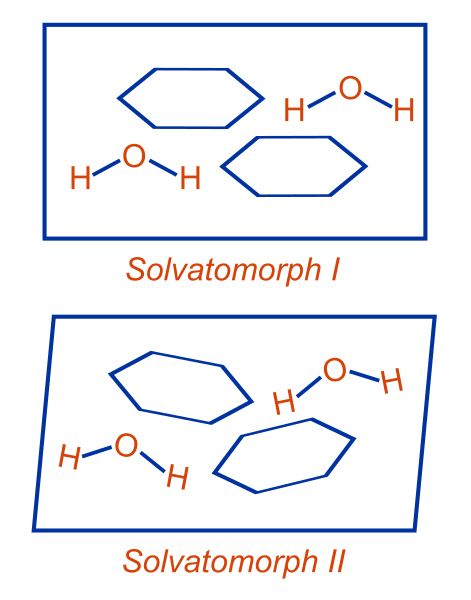
\includegraphics[width=8cm]{src/figures/intro_figs/solvatomorphs.png}
    \caption{Diagram of Solvatomorphs.}
    \label{solvatomorph_fig}
\end{figure}
\section{Density Functional Theory}
Density functional theory is a method of analysis that utilizes first principle, quantum mechanics calculations to investigate the electronic structure of materials \citep{baseden_introduction_2014,paul_true_2019}. Many physical and chemical properties are governed by the material's electronic states. DFT calculations provide accurate information about your system because the calculations take into account quantum mechanical effects, however, this trade-off in accuracy comes at a high computational cost compared to other simulation methods. DFT uses the electron density surrounding a particle to calculate the energy. The particles undergo a slight change in position and the energies are calculated again. This continues until the system's energy is at a minimum. 

\begin{figure}
    \centering
    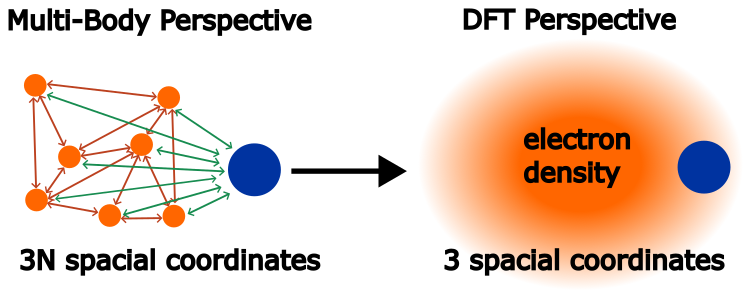
\includegraphics[width=12cm]{src/figures/intro_figs/dft_diagram.png}
    \caption{A depiction of how density functional theory simplifies the many-body problem into a function of electron density. }
    \label{DFT_diagram}
\end{figure}

DFT was developed upon the Hohenberg-Kohn theorems, the first of which was published in 1964 \citep{hohenberg_inhomogeneous_1964}. The first theorem states that the ground state properties, or energies, of a many body system can be calculated using only a functional ($F[n]$) of the electron density ($n(\textbf{r})$). This theorem reduced the many body problem of N particles from 3N spacial coordinates down to only 3 spacial coordinates. The electron density is defined in terms of the three spacial coordinates, shown in \autoref{DFT_diagram}. While the first theorem describes the possibility of calculating ground state properties from electron density it does not provide any information about the functional required to do so. The second Hohenberg-Kohn theorem states that if the exact functional of a system is known, the electron density that minimizes this functional will correspond to the exact solution of the Scrhodinger's equation \citep{kohn_self-consistent_1965}. Though the only system in which an exact functional has been proven is for a homogeneous electron gas, in all many-body systems the energy functional must be approximated. 
\subsection{Functionals and Basis Sets}
\autoref{eq_dft1} describes DFT in a mathematical sense, where $E_{v}[n]$ is equal to the ground state energy of the system and $v(\textbf{r})$ is the external potential. \autoref{eq_dft1} also details that the density functional $F[n(\textbf{r})]$ is independent of the external potential. 
\begin{equation}
    E_{v}[n] \equiv \int v(\textbf{r}) n(\textbf{r})d\textbf{r} + F[n(\textbf{r})]
    \label{eq_dft1}
\end{equation}
We can further examine the total energy of the system using \autoref{eq_dft2}. 
\begin{equation}
    E[\{\Psi_i\}] \equiv E_{known} [\{ \Psi_i \}] + E_{XC} [\{\Psi_i\}]
    \label{eq_dft2}
\end{equation}
The $E_{known}$ term includes the kinetic, potential, and hartree energy, all of which can be calculated exactly for a given system. The second term of \autoref{eq_dft2} includes the exchange-correlation energy $E_{XC}$. This energy is unknown for many-body systems and therefore has to be approximated using density functionals. The exchange-correlation energy can only be calculated for a homogeneous, uniform electron gas, with constant electron density, which is the system that Hohenberg and Kohn used to prove their first theorem, mentioned above \citep{hohenberg_inhomogeneous_1964}. Different systems may require different approximations, depending on the information you are trying to learn from your simulation. This makes choosing your functional one of the most important steps in a DFT investigation. For more complex systems various types of functionals exist, including the local density approximation (LDA), generalized gradient approximation (GGA) and hybrid functionals, among others \citep{goh_exchange-correlation_nodate, hasnip_density_2014}. LDA functionals are the most simplified models, they take into account only the electron density derived from a free electron gas. GGA functionals build on LDA functionals by also including information about the gradient observed in the electron density. This adds a level of complexity and accuracy for models that do not have uniform electron density. The functionals used in this body of work are hybrid functionals. Hybrid functionals combine the exact electron density of the system, derived by the Hartree-Fock theory, with the $E_{XC}$ from traditional DFT functionals, such as the GGA \citep{hybrid_2007, Heda_2023}. 
Along with choosing the functional, you must also determine a basis set to use in your DFT calculations. The basis set is set of basis functions that reduces calculations from partial derivatives to algebraic equations. Various types of basis sets exist, including plane-wave and atomic orbital. Atomic orbital basis sets place the basis equations on each atom in order to build the atomic orbitals. 
Chapters 2 and 3 detail how DFT was utilized to determine the crystalline configurations of two hydrate systems, violuric acid monohydrate and barbituric acid dihydrate, over a broad temperature range. Both hydrate systems had been suspected to exhibit polymorphism, but upon further investigation it was concluded that crystalline disorder was skewing the experimental results and the accurate crystalline configurations were determined using DFT geometry optimization calculations. 

\section{Organic Photovoltaics}
Photovoltaic (PV) devices are a promising solution to the rising energy crisis in America \citep{mazzio_future_2015}. Inorganic photovoltaic cells, often composed of silicon, have a relatively high production and implementation cost\citep{mazzio_future_2015}. Producing organic photovoltaic devices (OPVs) can be done at a potentially lower cost than silicon because the raw materials require less energy-intensive processing. Small molecule OPVs have recently achieved a photoelectric efficiency of almost 20\%, which has increased impressively over recent years \citep{sun_span_2022}. The Shockley-Quiesser limit suggests that there is still room for the power conversion efficiency of organic solar devices to increase by approximately 15\%, leading to a PCE of 35\% \citep{miller_strong_2012}. Introducing morphologies that have a higher charge carrier mobility have been proven to be the key to improving the cell’s PCE. 
Organic materials are typically not thought of as semiconductors, however, it is evident throughout biology that many organic molecules can function as semiconductors. For an organic material to act as a semiconductor the molecules must exhibit significant conjugation \citep{kularatne_donoracceptor_2013}. Conjugation is the presence of overlapping pi-orbitals that create a system of delocalized electrons. These delocalized electrons are more readily excitable and are not linked to one specific atom within the molecule. As the conjugation length increases in the material, the band gap decreases, meaning that the electrons require less energy to be excited into the conduction band. Once in the conduction band the electron can contribute to conductivity \citep{callister_materials_2010}. In order to excite an electron from the highest occupied molecular orbital (HOMO) to the lowest unoccupied molecular orbital (LUMO) the incident photon’s energy must be equal to or greater than the excitation energy. When an electron is excited into the LUMO, where it has enough energy to move about the surface of the molecule, there is a leftover ‘hole’ where the electron used to be. In comparison the the negative environment surrounding it, the hole has an effective positive partial charge. The electron and hole have a coulombic attraction due from their opposing charges, resulting in a force that binds the electron and hole together into what is called an exciton \citep{reis_effect_2022}.
\begin{figure}[ht]
    \centering
    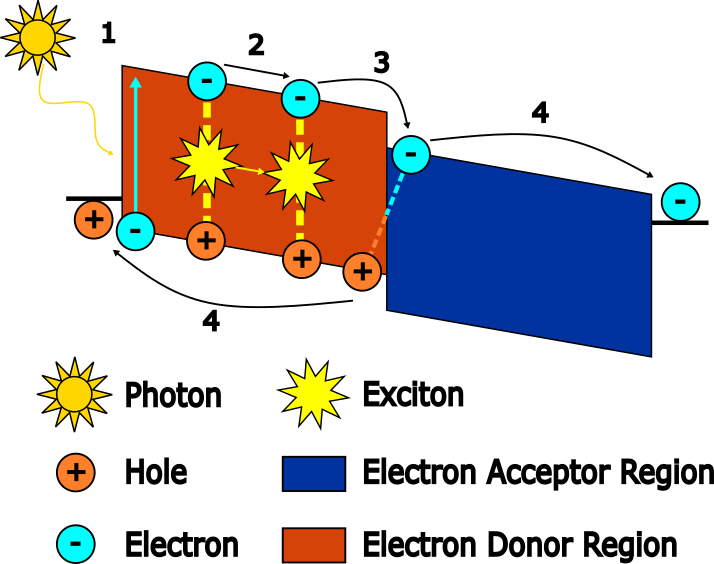
\includegraphics[width=10cm]{src/figures/intro_figs/OPV_Figure.png}
    \caption{Diagram of an OPV device. (1) Photon absorption (2) Exciton creation and migration (3) Exciton dissociation (4) Charge carrier diffusion.}
    \label{OPV_fig}
\end{figure}
\par The photoelectric effect, described above, is what makes OPV devices functional. In an OPV device, when an incident photon hits the surface it is passed through into the active layer, where an exciton is created (\autoref{OPV_fig}, step 1). The exciton diffuses through the active layer until it reaches a grain boundary between an acceptor region and donor region, where exciton dissociation occurs (\autoref{OPV_fig}, steps 2 \& 3). Once the coulombic connection between the electron and hole is broken the electron diffuses through the acceptor region to be harvested at the cathode and the hole through the donor region to be harvested at the anode (\autoref{OPV_fig}, step 4) \citep{Zhang2018}. 
\begin{wrapfigure}{r}{0.5\textwidth}
  \begin{center}
    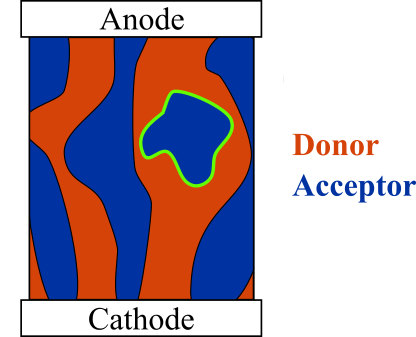
\includegraphics[width=0.48\textwidth]{src/figures/intro_figs/bulk_heterojunction.png}
  \end{center}
    \caption{Depiction of a bulk heterojunction (BHJ) active layer of an organic photovoltaic device. Outlined in green is a an "island" where the electron would have no access to the electrode, forcing it to recombine with a hole, rendering it useless.}
  \label{BHJ}
\end{wrapfigure}
\par The active layer motif depicted in \autoref{BHJ} is called a bulk heterojunction active layer \citep{gaspar_recent_2018}. These donor/acceptor regions can come from two different organic semiconductor molecules or a co-polymer with differing acceptor monomers and donor monomers \citep{piris_photogeneration_2009}. The donor/acceptor regions need to exhibit a significant difference in energy levels in order to cause exciton dissociation when the exciton crosses the grain boundary. Once the excitons are dissociated the charge carriers have to pass through the active layer to their respective anodes \citep{radford_controlling_2021}. If there is not a clear path for the electron or hole to travel to electrodes these charges are typically lost to exciton recombination. This is why the morphology of the active layer is so important to the power conversion efficiency. 
\par Understanding the influence of structural conformation on OPV device performance brings us to the importance of density functional theory calculations and molecular dynamics simulations. DFT has many applications, one of which is geometry optimizations of small molecule systems. From these geometry optimizations we can determine the most energetically favorable conformation of our system. Molecular dynamics (MD) simulations (as discussed below) are an efficient way to determine the morphology of the active layer and the properties associated with it \citep{chen_fluorination_2022}. MD simulations are used for investigating the structures of OPV active layers because they follow the self-assembly of the copolymers in a bulk heterojunction. MD simulations give us information about the thermodynamics of the self-assembly as well as the kinetics of how these molecules interact to form the equilibrium structures. MD simulations also have the benefit of simulating large molecule systems at a lower computational cost than DFT. The information gained from DFT calculations in conjunction with MD simulations can give great insight into how our copolymers will self-assemble during in the active layer during device production \citep{krebs_all_2009}. 

\section{Molecular Dynamics}
\par Molecular dynamics is a computational simulation method used to predict equilibrium morphologies of many particle systems. Newton's equations of motion are solved numerically to generate trajectories of how molecular systems evolve over time \citep{frenkel_understanding_2002}. 
The basic algorithm behind an MD simulation is: (1) calculate potentials and forces from particle positions. (2) Update particle velocities using the forces calculated in (1). (3) Update particle positions from the velocities calculated in (2). (4) Continue (1)-(3) with updated particle positions until equilibrium is achieved. 
Once equilibrium is achieved we  calculate the decorrelation time (time steps between independent samples) and calculate system properties by averaging independent microstates. 
\par The forces of attraction and repulsion enacted on one particle by another are described by the particles' pair potential. The pair potential is essentially the potential energy of two interacting particles. A common pair potential used in MD simulations is the Lennard-Jones (LJ) potential \citep{vollmayr-lee_introduction_2020,LJ_history}. The LJ-potential, depicted in \autoref{ljplot} and explained mathematically in \autoref{lj-equation}, describes the potential energy $U_{LJ}(r_{i,j})$ of two particles, $i$ and $j$, as a function of internuclear distance, $r_{i,j}$. 
\begin{figure}[ht]
    \centering
    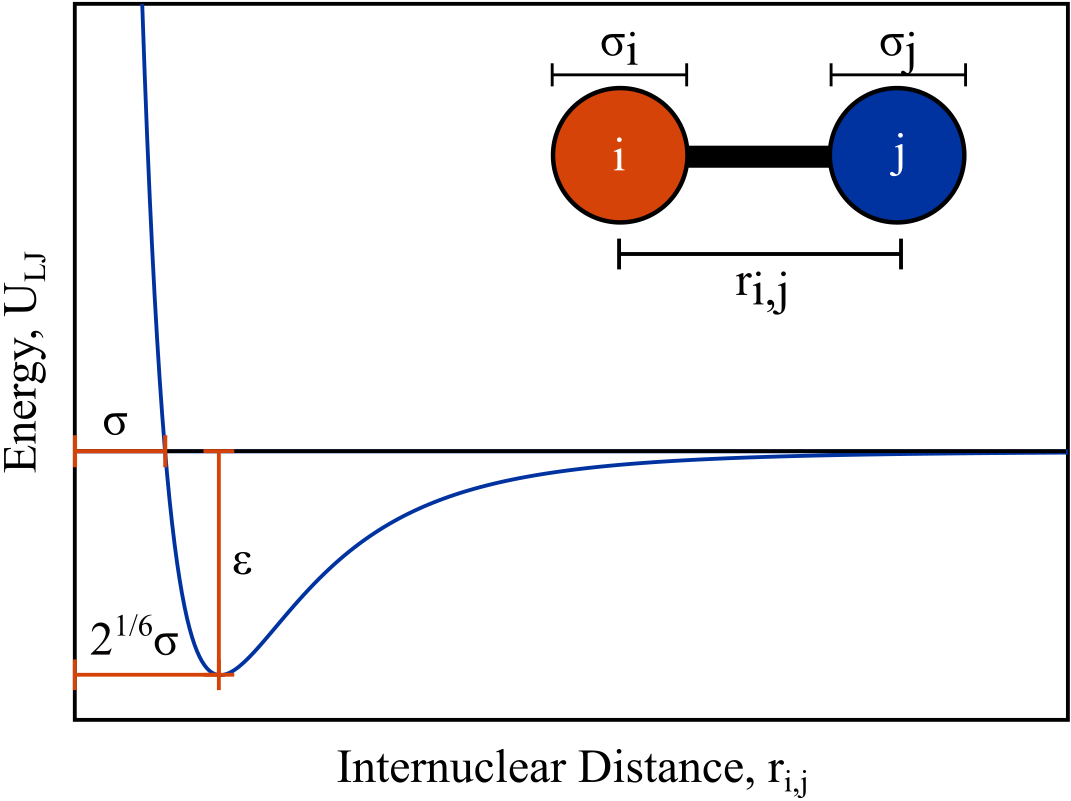
\includegraphics[width=12cm]{src/figures/intro_figs/LJ_pot.png}
    \caption{Plot of the Lennard-Jones potential energy.}
    \label{ljplot}
\end{figure}

\begin{equation}
    U_{LJ}(r_{ij}) = 4\epsilon \left[ \left({\frac{\sigma}{r_{ij}}}\right)^{12} - \left({\frac{\sigma}{r_{ij}}}\right)^{6} \right]
    \label{lj-equation}
\end{equation}

Pair interactions are governed by $\sigma$ and $\epsilon$. $\sigma$ is the internuclear distance at which the potential energy between two particles is zero and epsilon is the depth of the well in the potential energy plot. $\epsilon$ is a measure of how attractive the particle is and $\sigma$ can be thought of as the diameter of the particle. As shown in \autoref{ljplot}, the potential energy reaches a minimum when the particles are at a distance of $2^{1/6}\sigma$ apart. At distances closer than $2^{1/6}\sigma$, the particles repel one another and at distances greater than $2^{1/6}\sigma$ the the forces felt are negative, which accelerates the particles toward one another. The greater the distance gets from $2^{1/6}\sigma$, the lesser the effect the attractive force has on the other particle. In this study, we used the Lorentzian combination rule for sigma and a geometric combining rule for epsilon, shown in \autoref{comb_rule}. 

\begin{equation}
    \sigma_{i,j} = \frac{\sigma_{i} + \sigma{j}}{2}  ,   \epsilon_{i,j} = \sqrt{\epsilon_{i} * \epsilon_{j}}
    \label{comb_rule}
\end{equation}

Other properties, such as bond, angle and dihedral, also dictate how particles interact and how a system evolves over time. In MD simulations bonds and bond angles are described as harmonic oscillators, using \autoref{potE_bond_distance}, where $U(r)$ is the potential energy of the bond, $r$ is the internuclear distance between the bonded particles, $r_0$ is the equilibrium internuclear distance and $k_h$ is the bond's harmonic spring constant. A diagram depicting the bonds, angles, and dihedral angles is shown in \autoref{forces_fig}. 

\begin{equation}
    U(r) = \frac{1}{2} k_{h} \left( r - r_{0} \right)
    \label{potE_bond_distance}
\end{equation}
\autoref{potE_bond_angle} described the potential energy $U(\theta)$ associated with the bond angle, $\theta$, where $\theta_0$ is the equilibrium bond angle and $k_{\theta}$ is the harmonic angle constant. 
\begin{equation}
    U(\theta) = \frac{1}{2} k_{\theta} (\theta - \theta_{0})
    \label{potE_bond_angle}
\end{equation}
\begin{figure}[ht]
    \centering
    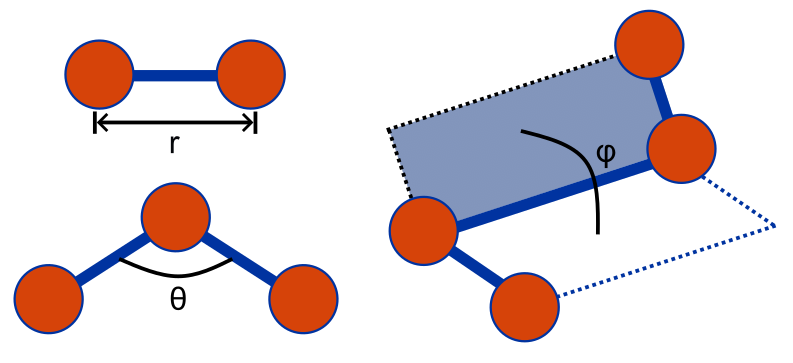
\includegraphics[width=0.5\linewidth]{src/figures/intro_figs/dihedral_fig.png}
    \caption{Illustration of bond distance (r), bond angle ($\theta$), and dihedral angle ($\phi$)}.
    \label{forces_fig}
\end{figure}
\par Dihedrals are described using \autoref{potE_dihedral}, where $k_n$ is the spring constant of the corresponding particle, $\phi$ is the angle between atoms planes within the dihedral, and $U(\phi)$ is the potential energy of the dihedral. 

\begin{equation}
    U(\phi) = \frac{1}{2}k_1(1+\cos(\phi)) + \frac{1}{2}k_2(1+\cos(2\phi)) + \frac{1}{2}k_3(1+\cos(3\phi)) + \frac{1}{2}k_4(1+\cos(4\phi))
    \label{potE_dihedral}
\end{equation}

In our simulation framework we try to follow the TRUE model, ensuring that our simulations are transparent, reproducible, usable and extensible. In MD simulations a forcefield is used to efficiently store and keep track of all the variables used in the pair, angle, bond, harmonic potentials mentioned above \citep{ghahremanpour_refinement_2022,gaff}. Each unique pair interaction requires its own unique set of parameters to model the pair of particles using the equations listed above. The process of creating and applying a forcefield is a common barrier to the transparency and reproducibility of our TRUE simulations \citep{jankowski_perspective_2020}. It is frequent in initializing a simulation of a new molecule to have missing forcefield parameters. In these cases the parameters must be either added to an existing forcefield file or a new forcefield file must be produced. In this study, we have developed a workflow that implements an open source software to create a forcefield file from a molecule graph \citep{wang_end--end_2022}. We have validated this workflow for complex, conjugated polymers by comparing simulation results of two molecules to previously published results (Chapter 4). After validating this workflow it was utilized to simulate 13 different complex polymers (Chapter 5).  

In comparison to MD simulations, DFT calculations come with a much higher computational cost. Due
to this, larger systems that can be equilibrated using MD cannot be simulated with DFT. On the other
hand, however, MD simulations often don’t provide as much information about a system as DFT
calculations do. This is due to the neglect of quantum effects in MD simulations. Due to these differences, in this dissertation we utilize DFT to predict the crystalline conformation of small molecules like BTADH and VAMH, but employ MD simulations to determine how macromolecules and polymers interact to self-assemble into bulk morphologies. In both cases, however, molecular simulations are used over experiment due to experimental constraints, such as difficulty in structure determination and experimental costs and time. The results from the molecular simulations are then used to direct experimental research toward materials of interest for the given application. 
%------------------------------------------------------------------------------
\chapter{True Polymorphic Phase Transition or Dynamic Crystal Disorder? An Investigation into the Unusual Phase Behavior of Barbituric Acid Dihydrate} 
The following chapter contains published work written by me with the guidance of Dr. Matthew King. This work is published at Ref. \citep{paul_true_2019}. 
\label{chap:BTADH}
\section{Abstract}
Crystalline barbituric acid dihydrate (BTADH) was previously thought to undergo a subtle temperature-dependent phase transition from a high-temperature orthorhombic \textit{Pnma} space group to a non-merohedrally twinned monoclinic \textit{P}2\textsubscript{1}/\textit{n} phase below a transition temperature of ~217 K. Questions remain on the true nature of the unusual transformation and the structure of the high-temperature crystal phase due to difficulties in resolving the \textit{Pnma} structure from X-ray diffraction data and because of the subtlety of the structural transition. In this study, terahertz (THz) spectroscopy and solid-state density functional theory (DFT) were utilized to explore this suspected phase transition and uncover the principle physical mechanisms contributing to this anomalous transition. Our findings suggest that at temperatures above the previously reported phase transition temperature of 217 K, the crystal does not exist in the \textit{Pnma} space group configuration. However, two equivalent favorable energetic states with \textit{P}2\textsubscript{1}/\textit{n} symmetry related by the twinning plane lie on either side of the proposed \textit{Pnma} structure. It is these same local potential energy minima that guide the crystal system to a non-merohedrally twinned configuration identified in the low-temperature crystal structures. At temperatures above 217 K, the system possesses the thermal energy necessary to readily transition between these degenerate states separated by the low-lying \textit{Pnma} structural barrier. The evidence acquired by THz spectroscopy and DFT indicate the absence of a true temperature-dependent phase change, and rather a system that exists in a tenuous thermally disordered state above the previously alleged transition temperature.
\section{Introduction}

The crystalline conformation of compounds can have a large influence on material properties, such as solubility, dissolution rate, melting point, and mechanical properties, and these can vary significantly between polymorphs of a compound \citep{Brittain2016,bernstein_polymorphism_2011,gentili_polymorphism_2019}. As polymorphism has a profound influence on such physicochemical properties, the study of the growth and transformation of polymorphs and solvatomorphs have become a quite impactful area of interest for pharmaceutical development, crystal engineering, and de novo materials design\citep{galindo_control_2017,maini_chemical_2015,hiremath_controlling_2005,cocca_influence_2011,lee_crystal_2011,moulton_molecules_2001,baskar_raj_pseudo-polymorphism_2003}. However, detailed experimental and computational analyses of complex target systems can often be difficult. In ongoing efforts to improve computational methodologies to describe the behavioral intricacies of crystal systems, it is useful to accompany such approaches with experimental spectroscopic analyses in the study of polymorphism, phase transitions, and related phenomena.
In this study, solid-state density functional theory (DFT) and terahertz (THz) spectroscopy were used to explore the underlying physical mechanisms leading to a subtle temperature-dependent phase transition exhibited by the barbituric acid dihydrate (BTADH) crystal system. THz spectroscopy has been shown to be a powerful tool for the investigation of molecular crystals and polymorphism since THz radiation can be used to probe phonon vibrations sensitive to the specific intermolecular interactions present in a particular molecular packing configuration \citep{ruggiero_resolving_2016,ruggiero_predicting_2018,king_understanding_2011,king_identification_2011,delaney_understanding_2012}. In combination with DFT calculations, valuable information can be obtained regarding structure, energetics, and vibrational properties \citep{ruggiero_concomitant_2017,allis_solid-state_2006}. 
Crystalline BTADH is reported to undergo a transition from a high-temperature orthorhombic \textit{Pnma} phase to a non-merohedrally twinned monoclinic \textit{P}2\textsubscript{1}/\textit{n} phase below a transition temperature of ~217 K (\autoref{BTADH_fig}). The BTADH system has been extensively studied by X-ray diffraction, with most attempts at resolving the high-temperature phase resulting in the investigators reluctantly coming to the same conclusions. The most thorough study was performed by Nichol and Clegg in 2005, whom measured the BTADH system at 14 temperatures ranging from 100–270 K, with meticulous focus on temperatures surrounding the suspected transition temperature reported at 216–217 K \citep{nichol_btadh_2005}. Most unusual is the subtlety of the phase transformation undergoing no changes in hydrogen bonding motifs upon the \textit{Pnma} to \textit{P}2\textsubscript{1}/\textit{n} transition, only an out-of-plane rotation of the barbituric acid molecules and modest displacements of the two H\textsubscript{2}O molecules and the sp3-hybridized carbon of barbituric acid. The authors ultimately determined a high-temperature \textit{Pnma} phase, which was in line with two preceding studies also proposing the \textit{Pnma} space group at room temperature \citep{1961_Jeffrey,1977_Al-Karaghouli}. These studies reported quite large atomic displacements along the b-axis, perpendicular to the mirror plane containing all atoms, besides the mirrored sp3 hydrogens. Furthermore, Al-Karaghouli et al. studied the BTADH system by neutron diffraction and proposed that the crystal may take a Pn21a configuration or that the H\textsubscript{2}O oxygen atoms may not lie within the mirror plane \citep{1977_Al-Karaghouli}. However, neither proposition gave satisfactory results, leading both studies to settle on the \textit{Pnma} space group assignment. All previous reports do agree that the BTADH crystal system at temperatures below 217 K adopts the \textit{P}2\textsubscript{1}/\textit{n} space group and exhibits non-merohedral twinning relating equivalent \textit{P}2\textsubscript{1}/\textit{n} unit cells by a two-fold rotation about the b-axis. 

\begin{figure}[ht]
  \center
  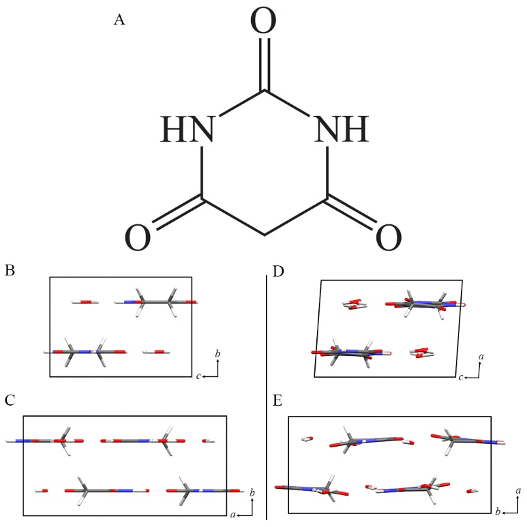
\includegraphics[width=7.5cm]{src/figures/btadh_figs/btadh_fig1.png}
  \caption{A) Molecular structure of barbituric acid. Comparison of the crystalline structures of the temperature-dependent BTADH polymorphs, with the high-temperature \textit{Pnma} form viewed along the B) a-axis and C) c-axis, and the low-temperature \textit{P}2\textsubscript{1}/\textit{n} form along the D) b-axis and E) c-axis.}
  \label{BTADH_fig}
\end{figure}


\section{\nobreak Experimental Section}
\subsection{THz Spectroscopy}
Anhydrous barbituric acid (BTA) was obtained from Sigma-Aldrich (99\% purity). BTADH was crystallized from a saturated aqueous solution by slow evaporation at room temperature over a period of one week under darkness. Samples for THz measurements were mixed with polytetrafluoroethylene (PTFE) powder at concentrations of approximately 4.5\% by mass. The samples were pulverized using a stainless steel amalgamator (Dentsply Rinn 3110-3A) to minimize particle size and scattering of THz radiation. Approximately 0.50 g of the sample mixtures were pressed into pellets under a measured pressure of 2000 psi using a hydraulic press (ICL EZ-Press 12) equipped with a 13 mm stainless steel die. PTFE pellets for use as reference blanks were prepared in the same manner. THz spectra were recorded using a custom time-domain pulsed THz spectrometer based on an amplified Ti:sapphire laser system (Coherent, Inc., Santa Clara, CA), described in detail elsewhere \citep{rexrode_effects_2019}. Data were acquired at 293 and 78 K with samples under vacuum. Samples and blanks were scanned 32 times and data were averaged for each individual data set. Each 32-ps scan window consisted of 3200 data points representing the THz waveform, producing an effective instrument resolution was approximately 1.0 cm\textsuperscript{-1}. The ratio of the power spectra obtained from the Fourier-transformed data sets of the sample and blank produced the THz absorption spectrum. Each THz spectrum presented in this work is the average of four individual THz spectra.

\subsection{Solid-State Density Functional Theory}

All calculations were performed using the Crystal14 software package \citep{Dovesi2014,Dovesi2017}. Solid-state DFT calculations utilized the PBE,\citep{perdew} M06,\citep{zhao_m06_2008} and B3LYP \citep{Lee_1988,becke_density-functional_1993} functionals with atom-centered cc-pVDZ,\cite{dunning_gaussian_1989} 6-31G(d,p),\citep{hehre_selfconsistent_1972,Hariharan1973TheIO} 6-311G(d,p),\citep{krishnan_self-consistent_1980} and pob-TZVP \citep{peintinger_consistent_2013} basis sets. Initial lattice dimensions and atomic coordinates were acquired from X-ray crystallographic data from Cambridge Crystallographic Database\citep{nichol_btadh_2005,groom_cambridge_2016}. The sampling rate as a function of k points used in defining the real space density matrix and Monkhorst grid in reciprocal space was determined for total energy convergence criteria of \(\Delta\)E \(<\) 10\textsuperscript{-8} hartree for geometry optimizations and \(\Delta\)E \(<\) 10\textsuperscript{-11} hartree for normal-mode calculations \citep{gilat_analysis_1972,monkhorst}. In order to meet these convergence criteria, shrinking factors of 6 where used for the BTADH crystal calculations. The total number of grid points varied between calculations depending on initial crystal geometry. The radial and angular distributions of points were defined by a pruned (75,974) integration grid for each calculation. A pair-wise (D2) damped empirical energy correction for London-type dispersion forces as proposed by Grimme et al \citep{grimme_accurate_2004,grimme_semiempirical_2006}. was included in all DFT calculations. The global scaling factors, s6, used for the dispersion correction term were 0.75, 0.25, and 1.05 for PBE, M06, and B3LYP, respectively \citep{zhao_m06_2008,grimme_accurate_2004,grimme_semiempirical_2006,Karton_2009}. Additional dispersion parameters, including C6 coefficients, van der Waals radii, cut-off distance, and dampening function steepness, were taken from Grimme et al \citep{grimme_accurate_2004,grimme_semiempirical_2006}. Modifications to van der Waals radii were made in accordance with Civalleri et al. \citep{civalleri_b3lyp_2008}. for the application of D2 dispersion corrections in molecular crystals. The truncation tolerances for the Coulomb and HF exchange integral series are defined by the program keyword TOLINTEG, and were set to values of 10\textsuperscript{-8}, 10\textsuperscript{-8}, 10\textsuperscript{-8}, 10\textsuperscript{-8}, and 10\textsuperscript{-16} hartree. Frequencies of normal modes were calculated within the harmonic approximation by numerical differentiation of the analytical gradient of the potential energy with respect to atomic position\citep{pascale_calculation_2004}. The IR intensities for normal modes were calculated from the dipole moment derivatives (d$\mu$/dQ) determined by the Berry phase approach of calculating Born charges as polarization differences between equilibrium and distorted geometries \citep{zicovichwilson_calculation_2004}.

\section{Results and Discussion}
An initial screening of density functional and basis set combinations was performed to determine those best suited to reproduce the experimental X-ray crystal structures of BTADH by solid-state DFT. The PBE, M06, and B3LYP density functionals were employed, representing GGA, meta-GGA, and hybrid classes of functionals, respectively. Each density functional was combined with two different commonly used double-\(\zeta\) basis sets – 6-31G(d,p) and cc-pVDZ – and two triple-\(\zeta\) basis sets – 6-311G(d,p) and pob-TZVP. Geometry optimizations were performed in both fixed lattice dimensions of the 100-K structure and full-cell optimizations allowing lattice parameters to freely optimize within the constraints of space group symmetry. The 100-K X-ray crystal structure in \textit{P}2\textsubscript{1}/\textit{n} was used as the starting point for all calculations. \textit{Pnma} unit cells of the high-temperature crystal phase were not used for this initial evaluation as the crystal structures in \textit{Pnma} symmetry confine the BTA and H\textsubscript{2}O molecular orientations to planar configurations, thus no valuable information into functional/basis set performance can be obtained regarding intermolecular interactions from such calculations. The quality of structural reproduction was based on the notable structural variations presented through the suspected temperature-dependent phase transition using the series of BTADH crystal structures over the temperature range of 100–270 K reported in Ref. 18. For the geometry optimizations in fixed lattice dimensions, the angle between molecular planes between BTA molecules within a unit cell, the deviation of the CH\textsubscript{2} group from the BTA molecular plane, and the angle of planes formed by each of the two water molecules in the dihydrate asymmetric unit were used as metrics for structural reproduction (\autoref{btadh_planeorientations}). For full-geometry optimizations, lattice parameters a, b, c, and \(\beta\) were evaluated in addition to the aforementioned conformational metrics. These data for the experimental X-ray structures are provided in \autoref{btadh_latticeparams}.

\begin{figure}
  \center
  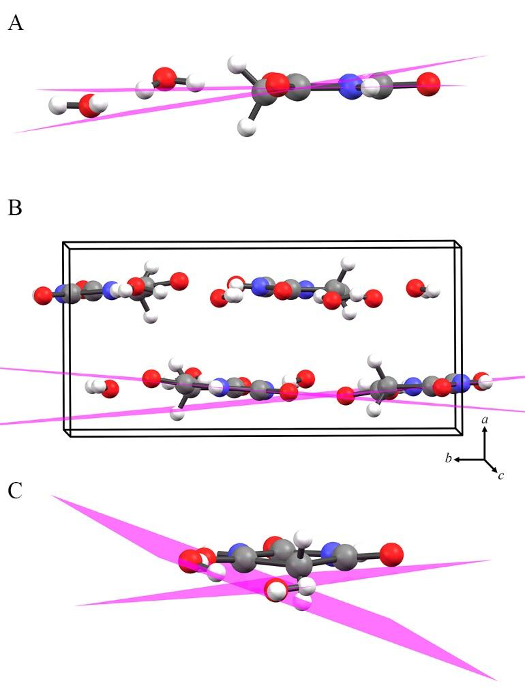
\includegraphics[width=7.5cm]{src/figures/btadh_figs/btdah_fig2.png}
  \caption{Plane orientations relating angle metrics for determining the quality of unit cell reproductions. A) BTADH molecular plane defined by ring carbonyl carbons, and that representing out-of-plane position of the ring CH\textsubscript{2} group. B) Opposing molecular planes of two symmetry-related BTADH molecules in the low-temperature \textit{P}2\textsubscript{1}/\textit{n} polymorph. C) Planes each created by a single H\textsubscript{2}O molecule of the dihydrate asymmetric unit.}
  \label{btadh_planeorientations}
\end{figure}

\begin{table}[ht]
  \centering
  \tiny
  \caption{Lattice parameters and calculated relative molecular orientations from BTADH experimental X-ray crystal structures reported in Ref. \citep{nichol_btadh_2005}.}
    \begin{tabular}{cccccccccc}
    \multicolumn{10}{l}{\textbf{Experimental X-ray}} \\
    \hline
    & \textbf{Space}  & & & & & & \textbf{CH\textsubscript{2}-} & \textbf{Mol-Mol} & \textbf{H\textsubscript{2}O-}\\
    \textbf{T (K)} & \textbf{Group} &	\textbf{a (Å)} & \textbf{b (Å)} & \textbf{c (Å)} & \textbf{\(\beta\)(°)} & \textbf{V (Å\textsuperscript{3})} & \textbf{Mol (°)\textsuperscript{a}} & \textbf{(°)\textsuperscript{b}} &	\textbf{H\textsubscript{2}O (°)\textsuperscript{c}} \\
    
    270 & \textit{Pnma}  & 6.2144 & 12.7512 & 8.8841 & 90 & 703.99 & -- & -- & -- \\
    230 & \textit{Pnma}  & 6.1739 & 12.7594 & 8.8831 & 90 & 699.77 & -- & -- & -- \\
    220 & \textit{Pnma}  & 6.1665 & 12.7630 & 8.8814 & 90 & 699.00 & -- & -- & -- \\
    219 & \textit{Pnma}  & 6.1624 & 12.7570 & 8.8780 & 90 & 697.90 & -- & -- & -- \\
    218 & \textit{Pnma}  & 6.1626 & 12.7570 & 8.8760 & 90 & 697.80 & -- & -- & -- \\
    217 & \textit{Pnma}  & 6.1770 & 12.7850 & 8.8980 & 90 & 702.70 & -- & -- & -- \\
    216 & \textit{P}2\textsubscript{1}/\textit{n} & 6.1567 & 12.7330 & 8.8650 & 91.180 & 694.80 & 1.85 & 2.98 & 28.87 \\
    215 & \textit{P}2\textsubscript{1}/\textit{n} & 6.1580 & 12.7514 & 8.8763 & 91.263 & 696.83 & 2.47 & 2.97 & 8.85 \\
    210 & \textit{P}2\textsubscript{1}/\textit{n} & 6.1538 & 12.7470 & 8.8770 & 91.627 & 696.00 & 2.85 & 3.6 & 20.31 \\
    200 & \textit{P}2\textsubscript{1}/\textit{n} & 6.1313 & 12.7030 & 8.8456 & 92.187 & 688.50 & 3.72 & 5.11 & 26.94 \\
    190 & \textit{P}2\textsubscript{1}/\textit{n} & 6.1377 & 12.7306 & 8.8641 & 92.528 & 691.94 & 4.81 & 5.9 & 16.72 \\
    170 & \textit{P}2\textsubscript{1}/\textit{n} & 6.1270 & 12.7253 & 8.8633 & 93.068 & 690.06 & 5.8 & 7.18 & 20.06 \\
    150 & \textit{P}2\textsubscript{1}/\textit{n} & 6.1130 & 12.7149 & 8.8564 & 93.437 & 687.14 & 6.7 & 8.22 & 25.09 \\
    100 & \textit{P}2\textsubscript{1}/\textit{n} & 6.0970 & 12.7152 & 8.8587 & 94.051 & 685.05 & 8.14 & 9.96 & 27.36 \\
    \hline
    \multicolumn{10}{l}{\textbf{DFT Full-Cell Geometry Optimizations in P2\textsubscript{1}/n}} \\
    & & & & & & & \textbf{CH\textsubscript{2}-} & \textbf{Mol-Mol} & \textbf{H\textsubscript{2}O-}\\
     \multicolumn{2}{c}{} &	\textbf{a (Å)} & \textbf{b (Å)} & \textbf{c (Å)} & \textbf{\(\beta\)(°)} & \textbf{V (Å\textsuperscript{3})} & \textbf{Mol (°)\textsuperscript{a}} & \textbf{(°)\textsuperscript{b}} &	\textbf{H\textsubscript{2}O (°)\textsuperscript{c}} \\
    \multicolumn{2}{c}{PBE/6-311G(d,p)} & 5.9263 & 12.6285 & 8.7625 & 94.455 & 653.81 & 8.76 & 10.53 & 24.04 \\
    \multicolumn{2}{c}{PBE/pob-TZVP} & 6.0755 & 12.4857 & 8.6603 & 94.438 & 654.97 & 11.39 & 15.53 & 40.25 \\
    \hline
    \multicolumn{10}{l}{\textsuperscript{a}CH\textsubscript{2}-Molecule planes (Fig. 2A); \textsuperscript{b}Molecule-molecule planes (Fig. 2B); \textsuperscript{c}Water-water planes (Fig. 2C).}
    \label{btadh_latticeparams}
    \end{tabular}
    \end{table}


It was determined from the extensive series of DFT structural calculations that the PBE density function in conjunction with the tested triple-\(\zeta\) basis sets, 6-311G(d,p) or pob-TZVP, were best suited for the computational treatment of the BTADH crystal system. The results of the computational screening are provided as \textbf{Supporting Information}. All subsequent calculations in this study utilized PBE/6-311G(d,p) and PBE/pob-TZVP. Results of the full unit cell geometry optimization using these functional/basis set combinations are also provided in \textbf{\autoref{btadh_latticeparams}}.
THz spectra of BTADH in the range of 20–95 cm\textsuperscript{-1} were obtained at 293 K and 78 K (\autoref{btadh_thz}A). Notable differences are present between the spectra taken at the two temperatures. At room-temperature, there is an absence of definitive spectral features below the one resolved peak at 88.8 cm\textsuperscript{-1}. Upon cooling to 78 K, six additional features emerge in the THz spectrum. Most conspicuous is the relatively narrow peak appearing at 33.6 cm\textsuperscript{-1} for which no evidence of any corresponding absorption intensity is present at 293 K. Large changes between THz spectra collected at different temperatures are usually indicative of a phase transformation leading to the activation/deactivation of phonon modes corresponding to the distinctive crystalline phases. In this case, however, there is not clear evidence of a phase transition between 293 and 78 K as many similarities remain between the two spectra, although many modes seem to be washed out at room temperature. There is an indication of underlying modes across the 293 K spectrum as broad absorptions resulting in a mostly featureless background that become resolved at low temperature. There is also a clear shift in the 88.8 cm\textsuperscript{-1} feature at 293 K to higher frequency upon cooling, which is typically observed temperature-dependent behavior for phonon modes.

\begin{figure}[h!]
  \center
  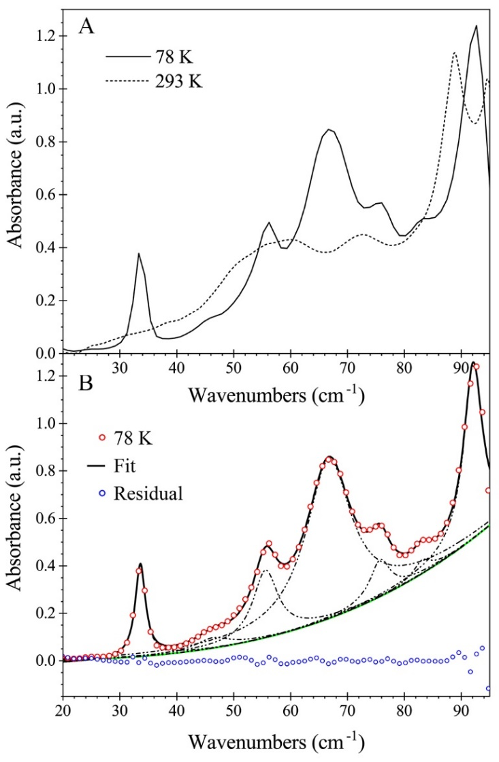
\includegraphics[width=6.5cm]{src/figures/btadh_figs/btadh_fig3.png}
  \caption{A) THz vibrational spectra of BTADH in the spectral range of 20-95 cm\textsuperscript{-1} obtained at 293 K and 78 K. B) Spectral fitting of the 78 K THz spectrum (red circles) with Lorentzian peaks (dashed lines) on exponential background (green line). The residuals of the experimental data and fitted values are indicated by blue circles.}
  \label{btadh_thz}
\end{figure}
\newpage
Another peculiar observance in the BTADH THz spectra collected at 78 K are the extremely broad symmetric absorptions between 40 and 80 cm\textsuperscript{-1}, and the discrepancy between linewidths of all present spectral features. A multiple peak fitting procedure was performed to determine the FWHM of the absorptions. Lorentzian line shapes for the seven distinguishable features were added to an exponential function representing the rising background, which is a product of Mie and Rayleigh scattering of THz radiation from the granular polycrystalline sample \citep{shen_elimination_2008}. The Lorentzian peaks and background were simultaneously fit to the experimental spectrum (\autoref{btadh_thz}B). Peak centers and FWHMs are provided in \autoref{thz_peaks}. The exponential function of form I=A\(\upsilon\)\^b , where I is the scattering intensity, A is the scalar accounting for particle size distribution, and b is the exponential factor influencing the frequency-dependence of scattering, yielded optimal values of A = 1.7 × 10\textsuperscript{-7} and b = 3.34. This value of b is in accordance with previously reported values using the same exponential form to correct for scattering effects observed in THz spectra \citep{king_identification_2011, shen_elimination_2008}.

\begin{table}[htbp]
\centering
\caption{Central frequencies and linewidths of THz spectral features in the range of 20 – 95 cm\textsuperscript{-1} for data collected at 78 K.}
\begin{tabular}{cc}
\textbf{Peak Center (cm\textsuperscript{-1})} & \textbf{FWHM (cm\textsuperscript{-1})} \\
\hline
33.6 & 2.2 \\
46.3 & 7.3 \\
55.6 & 5.4 \\
66.7 & 9.7 \\
75.7 & 4.3 \\
83.1 & 3.6 \\
92.1 & 4.0 \\	
\hline
\end{tabular}
\label{thz_peaks}
\end{table}

\par The spectral fitting routine resulted in a high-quality fit to the THz spectrum. Large deviations in FWHMs were determined for the observed peaks, ranging from 2.2 cm\textsuperscript{-1} for the mode centered at 33.6 cm\textsuperscript{-1} to a FWHM of 9.7 cm\textsuperscript{-1} for the 66.7 cm\textsuperscript{-1} feature. Peak symmetries and the quality of fit using single Lorentzian functions suggests that all seven resolvable features, including the broad absorption at 66.7 cm\textsuperscript{-1}, are due to single vibrational mode and not the product of contributions from multiple underlying modes. Such large discrepancies in peak widths are not typically observed in THz spectra of organic materials, although phonon mode softening along phase transition coordinates and a corresponding reduction in vibrational lifetimes can result in homogeneous broadening of peaks \citep{leguy_dynamic_2016,2008_Correa}. Changes in peak width are typically observed as the system nears a phase transition temperature \citep{la-o-vorakiat_phonon_2016}. However, this would not be expected for BTADH in the THz spectrum collected at 78 K, as this temperature is well below the suspected phase transition at ~217 K. 
Phonon vibrational frequencies were calculated by solid-state DFT to provide information on mode characters to aid in explanation of the unusual mode behavior exhibited by BTADH. Both triple-\(\zeta\) basis sets, pob-TZVP and 6-311G(d,p), that best performed for the initial structural evaluations were applied with the PBE density functional for normal mode calculations. The high-temperature crystal phase in \textit{Pnma} symmetry produced three imaginary vibrational frequencies in calculations utilizing either basis set. Examination of the atom displacement eigenvectors for each imaginary mode revealed that the most atomic motions are normal to the reflection plane imposed by the \textit{Pnma} space group for all atoms confined by this symmetry operator (\autoref{doublewell}). Scanning of the potential energy surface along the imaginary modes produces a symmetric double-well potential with a low lying energy barrier (\autoref{doublewell}A). Displacement of BTADH to either side of this double-well potential places the crystal into corresponding \textit{P}2\textsubscript{1}/\textit{n} structures related by a two-fold rotation about the b-axis, which is equivalent to the low-temperature phase. 
\newpage
\begin{figure}[h!]
  \center
  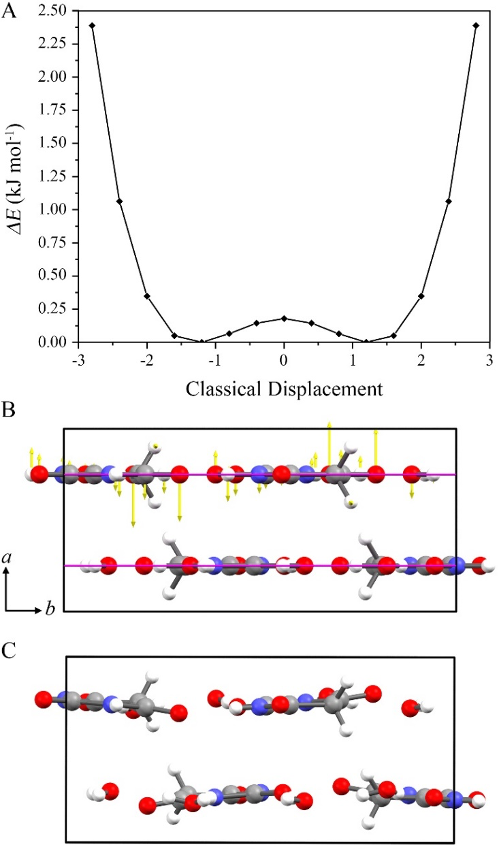
\includegraphics[width=7.5cm]{src/figures/btadh_figs/btadh_fig4.png}
  \caption{A) Scan of potential energy surface along the -35.79 cm\textsuperscript{-1} imaginary phonon mode (PBE/pob-TZVP) of BTADH confined to the \textit{Pnma} space group at 270-K lattice parameters. B) Displacement vectors (yellow arrows, magnitudes scaled ×10) for the imaginary mode shown for top two BTADH units. Displacements are oriented normal to the reflection plane (purple line) confining the molecules in \textit{Pnma} symmetry. C) Molecular orientation of BTADH optimized in \textit{P}2\textsubscript{1}/\textit{n} symmetry.}
  \label{doublewell}
\end{figure}
\newpage
\par Starting from the planar 270-K \textit{Pnma} crystal structure, symmetry constraints were removed and the geometry was re-optimized within fixed experimental X-ray lattice dimensions using PBE/pob-TZVP. The unit cell symmetry was relaxed to \textit{P}2\textsubscript{1}/\textit{n}, analogous to the suspected low-temperature phase, thus removing the reflection planes that confine the atoms in the \textit{Pnma} space group. From the optimized geometry, the measured molecular plane angles, as described in \autoref{btadh_planeorientations} and \autoref{btadh_latticeparams}, were 7.93°, 11.79°, and 36.82° corresponding to CH\textsubscript{2}–molecule, molecule–molecule, and H\textsubscript{2}O–H\textsubscript{2}O planes, respectively. These angles are remarkably similar to those observed for the X-ray crystal structures collected at low temperature. The relaxed-symmetry structural optimizations were repeated for each of the crystal dimensions measured at the 14 different temperatures in the range of 100–270 K using both the pob-TZVP and 6-311G(d,p) basis sets (\autoref{btadh_angles_table}). Analysis of the optimized geometries revealed little variation in measured angles over the temperature range. There was a general trend of angles increasing with decreasing temperature, but with no significant variations occurring between adjacent temperature steps.
An additional series of calculations were performed using the lattice dimensions of the suspected \textit{Pnma} phase, i.e. at temperatures above 217 K. The crystal structures were restricted to either \textit{P}2\textsubscript{1}/\textit{n} or \textit{Pnma} symmetry to evaluate differences in unit cell energies between the two crystal settings. In both basis sets, the \textit{P}2\textsubscript{1}/\textit{n}  symmetry produced the lower energy unit cell for all temperature lattice parameters (\autoref{E_pobtzvp}). The difference in energy between the \textit{P}2\textsubscript{1}/\textit{n} or \textit{Pnma} space groups were small in each case, ranging from -0.985 to -1.379 kJ mol-1 in the pob-TZVP basis, and -0.804 to -1.234 kJ mol\textsuperscript{-1} in 6-311G(d,p). These results show a slight energetic preference to \textit{P}2\textsubscript{1}/\textit{n} symmetry in unit cell dimensions at all temperatures above 216 K.

\begin{table}[htbp]
\centering
\tiny
\caption{Angles between the molecular planes of two molecules within the packed unit cell, angles between the two water molecules within the unit cell and the angles between the CH\textsubscript{2} plane and the molecular plane of one molecule.}
\begin{tabular}{cccccccccc}
\multicolumn{4}{c}{\textbf{CH\textsubscript{2}-Molecule\textsuperscript{a}(°)}} & \multicolumn{3}{c}{\textbf{Molecule-Molecule\textsuperscript{b} (°)}} & \multicolumn{3}{c}{\textbf{H\textsubscript{2}O-H\textsubscript{2}O\textsuperscript{c}(°)}} \\
\hline
& \textbf{pob-} & & & \textbf{pob-} & & & \textbf{pob-} \\
\textbf{T (K)} & \textbf{TZVP} & \textbf{6-311G(d,p)} & \textbf{exp.}  & \textbf{TZVP} & \textbf{6-311G(d,p)} & \textbf{exp.}  & \textbf{TZVP} & \textbf{6-311G(d,p)} & \textbf{exp.} \\
270 & 7.93 & 8.40 & --    &  11.79 & 11.27 & --     &  36.82 & 35.86 & -- \\
230 & 7.48 & 7.80 & --    &  11.19 & 10.55 & --     &  34.67 & 33.19 & -- \\
220 & 7.39 & 7.67 & --    &  11.07 & 10.41 & --     &  34.27 & 32.70 & -- \\
219 & 7.38 & 7.66 & --    &  11.12 & 10.43 & --     &  34.22 & 32.75 & -- \\
218 & 7.39 & 7.67 & --    &  11.14 & 10.45 & --     &  34.29 & 32.82 & -- \\
217 & 7.39 & 7.57 & --    &  10.88 & 10.19 & --     &  34.09 & 32.26 & -- \\
216 & 8.35 & 8.70 & 1.85  &  11.77 & 11.20 & 2.98   &  35.07 & 33.59 & 28.87 \\
215 & 8.34 & 8.63 & 2.47  &  11.57 & 10.95 & 2.97   &  34.65 & 32.86 & 8.85 \\
210 & 8.62 & 8.85 & 2.85  &  11.71 & 11.06 & 3.60   &  34.67 & 32.66 & 20.31 \\
200 & 9.12 & 9.39 & 3.72  &  12.25 & 11.70 & 5.11   &  35.20 & 33.53 & 26.94 \\
190 & 9.35 & 9.50 & 4.81  &  12.08 & 11.46 & 5.90   &  34.87 & 32.66 & 16.72 \\
170 & 9.65 & 9.79 & 5.80  &  12.17 & 11.56 & 7.18   &  34.53 & 32.07 & 20.06 \\
150 & 9.83 & 9.94 & 6.70  &  12.20 & 11.63 & 8.22   &  34.16 & 31.62 & 25.09 \\
100 & 10.05 & 10.02 & 8.14  & 12.06 & 11.44 & 9.96  & 33.22 & 30.19 & 27.36 \\
\hline
\multicolumn{10}{l}{\textsuperscript{a,b,c}Refer to Fig. 2 for plane definitions:  \textsuperscript{a}Fig. 2A; \textsuperscript{b}Fig. 2B; \textsuperscript{c}Fig. 2C.} \\
\label{btadh_angles_table}
\end{tabular}
\end{table}



\begin{table}[ht]
    \centering
    \begin{tabular}{ccc}
        \textbf{T(K)\textsuperscript{a}}    &   \textbf{\(\Delta\)E/pob-TZVP} &   \textbf{\(\Delta\)E/6-311G(d,p)}     \\
        \hline
        270     &   -1.379      &   -1.234          \\
        230     &   -1.116      &   -0.893          \\
        220     &   -1.050      &   -0.844          \\
        219     &   -1.050      &   -0.860          \\
        218     &   -1.050      &   -0.866          \\
        217     &   -0.985      &   -0.804          \\
        \hline
        \multicolumn{3}{l}{\textsuperscript{a}Lattice parameters for unit cells at variable}\\
        \multicolumn{3}{l}{temperatures are listed in \autoref{btadh_latticeparams}.}
    \end{tabular}
    \caption{Calculated energies (per BTA·2H\textsubscript{2}O) of BTADH confined to P2\textsubscript{1}/n and \textit{Pnma} symmetry groups at experimental lattice parameters. \(\Delta\)E provided in units of kJ mol\textsuperscript{-1}.}
    \label{E_pobtzvp}
\end{table}



THz vibrational frequencies were calculated for the low-temperature \textit{P}2\textsubscript{1}/\textit{n} phase using the fully relaxed unit cell structures (lattice dimensions provided in \autoref{btadh_latticeparams}) in PBE/pob-TZVP and PBE/6-311G(d,p) (\autoref{btadh_thz2}). The computed mode frequencies were mostly overestimated in comparison to the THz spectrum obtained at 78 K (\autoref{intensities}). This is typical in such calculations as the lattice dimensions used for normal mode calculations are contracted from the actual experimental dimensions due to neglect of thermal expansion in the DFT-optimized unit cells and contributions from basis set superposition error \citep{king_application_2011,king_modified_2012}. The result of constricting the unit cell dimensions is the general blue-shifting of vibrational frequencies as extensively shown in previous reports. In addition, vibrational anharmonicity of phonon modes contributes to overestimation of normal modes calculated in a harmonic limit \citep{ruggiero_resolving_2016,kleist_terahertz_2019,king_investigating_2010}. Frequencies were scaled by 0.80 in the spectral overlays provided in \autoref{btadh_thz2} to aid in visual comparison. Lorentzian lineshapes were convolved into calculated modes using the FWHM of the 33.6 cm\textsuperscript{-1} spectral feature to emphasize the large differences in linewidths observed in the THz spectrum. From the spectral simulations, the vibrational modes contributing to the observed THz absorptions can be assigned. A notable discrepancy between the phonon frequencies calculated by the two basis sets is the underestimation of the mode corresponding to the 33.6 cm\textsuperscript{-1} peak when using the 6-311G(d,p) basis set.

\begin{table}[ht]
    \centering
    \caption{Calculated phonon mode frequencies and intensities of full-relaxed BTADH unit cell in \textit{P}2\textsubscript{1}/\textit{n} symmetry using the PBE functional with the pob-TZVP and 6-311G(d,p) basis sets. }
    \begin{tabular}{c|c|c|c|c}
    \textbf{pob-TZVP} & \textbf{Int\textsuperscript{a}} & \textbf{6-311G(d,p)} & \textbf{Int} \\
    \hline
    43.46\textsuperscript{b} & 5.14 & 30.14 & 3.16 \\
    54.47 & 0.01 & 44.05 & 0.13 \\
    61.43 & 0.04 & 58.89 & 0.00 \\
    67.17 & 1.86 & 65.13 & 0.69 \\
    78.70 & 0.40 & 72.49 & 0.13 \\
    85.07 & 10.35 & 80.62 & 9.81 \\
    103.23 & 0.00 & 82.94 & 35.50 \\
    107.29 & 15.68 & 96.21 & 2.57 \\
    121.83 & 28.40 & 110.36 & 27.21 \\
    122.75 & 4.41 & 115.01 & 1.97 \\
    \hline
    \multicolumn{4}{l}{\textsuperscript{a}Intensity (km mol\textsuperscript{-1}); \textsuperscript{b}Frequency (cm\textsuperscript{-1})} \\

    \end{tabular}
    \label{intensities}
\end{table}
\newpage
\begin{figure}[h!]
  \center
  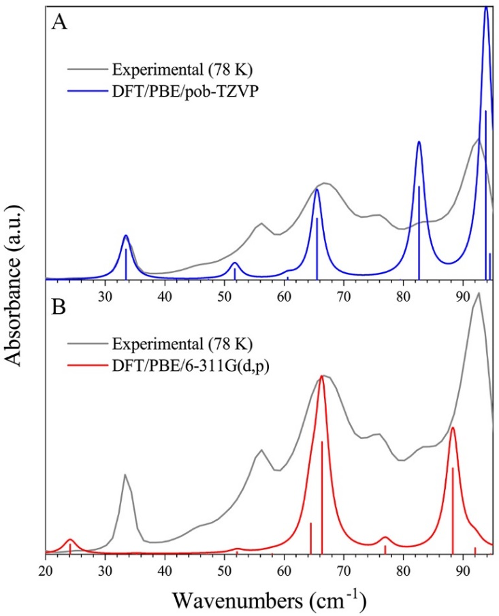
\includegraphics[width=10cm]{src/figures/btadh_figs/btadh_fig5.png}
  \caption{A) Mode character of the spectral feature at 33.6 cm\textsuperscript{-1} observed in the 78 K THz spectrum, represented by calculated displacement vectors (yellow arrows, magnitudes scaled ×10). B) Calculated mode displacements of the broad feature centered at 66.7 cm\textsuperscript{-1} in the 78 K THz spectrum. C) Mode character of the distinct 88.8 cm\textsuperscript{-1} vibrational mode observed in the 293 K THz spectrum (corresponding to the feature located at 92.7 cm\textsuperscript{-1} in the 78 K spectrum).}
  \label{btadh_thz2}
\end{figure}
\newpage
Of primary interest to explain the unexpected behavior of BTADH are the mode characters of the THz absorptions at 33.6, 66.7, and 92.1 cm\textsuperscript{-1}. The respective assignments of these modes were made by inspection of the spectral overlays, and are the 43.46, 85.07, and 121.83 cm\textsuperscript{-1} modes for PBE/pob-TZVP and the 30.14, 82.94, and 110.36 cm\textsuperscript{-1} modes for PBE/6-311G(d,p). Comparison of the vibrational motions for the assigned modes between the two basis sets confirms that these are indeed analogous modes. To reiterate the significance of these specific phonon vibrations, the 33.6 cm\textsuperscript{-1} mode appears in the THz spectrum at low temperature, but is ostensibly absent at room-temperature. The absorption at 66.7 cm\textsuperscript{-1} is unusually broad and is also not directly evident at room temperature. The 92.1 cm\textsuperscript{-1} mode, which is located at 88.8 cm\textsuperscript{-1} at room temperature, is present in the THz spectra at both 78 and 293 K and exhibits seemingly typical temperature-dependent phonon behavior. 
The calculated eigenvectors for each of the three normal modes are shown in \autoref{fig:btadh_vib_vectors}. It can be seen that the 33.6 and 66.7 cm\textsuperscript{-1} modes are along the direction of the suspected phase change relating the \textit{P}2\textsubscript{1}/\textit{n} and \textit{Pnma} symmetry cells perpendicular to the $\langle 100 \rangle$ lattice plane (\textit{P}2\textsubscript{1}/\textit{n} bc plane). The difference in the modes principally lies in the relative molecular translational and rotational contributions to each. The 33.6 cm\textsuperscript{-1} mode has primarily translational character with neighboring BTA molecules moving in opposing phase. The 66.7 cm\textsuperscript{-1} exhibits the adjacent BTA molecules rotating in-phase along the c-axis about their respective molecular centers of mass. In combination with the associated motions of the two H\textsubscript{2}O molecules, this vibration moves along a minima of the potential energy surface represented by the double-well potential shown in \autoref{doublewell}A relating two equivalent energetic minima. Finally, the vibrational mode corresponding the peaks at 88.8 and 92.7 cm\textsuperscript{-1} in the 293 K and 78 K spectra, respectively, consists of combined internal deformation of the BTA molecule, notably in the CH\textsubscript{2} groups, mixed with rotational character about the a-axis. The H\textsubscript{2}O molecular motions are both translational and rotational in character.

\begin{figure}[h!]
    \centering
    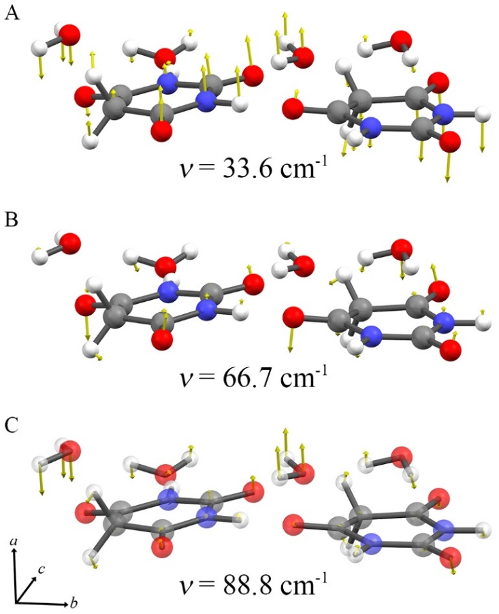
\includegraphics[width=0.5\linewidth]{src/figures/btadh_figs/btadh_fig6.png}
    \caption{(A) Mode character of the spectral features at 33.6 cm\textsuperscript{-1} observed in the 78 K THz spectrum, represented by calculated displacement vectors (yellow arrows, magnitudes scaled ×10). (B) Calculated mode displacements of the broad feature centered at 66.9 cm\textsuperscript{-1} in the 78 K THz spectrum. (C) Mode character of the distinct 88.8 cm\textsuperscript{-1} vibrational mode observed in the 293 K THz spectrum (corresponding to the feature located at 92.7 cm\textsuperscript{-1} in the 78 K spectrum).}
    \label{fig:btadh_vib_vectors}
\end{figure}

The unusual THz spectra obtained for BTADH can be explained by examining the vibrational mode characters. In the room-temperature spectrum, phonon modes having displacements primarily along the a-axis and are of rotational and translational character are not distinctly present, although a very broad absorption profile across the collection bandwidth is observed. The one distinct spectral feature at 293 K is due to a vibrational mode containing to a large extent intramolecular deformations, making it nearly independent of the barrier transition coordinate. We propose that subtle crystal disorder exists at higher temperatures about the low-energy barrier lying on the 〈100〉 lattice plane, or equivalently, the mirror plane confining the crystal system in imposed \textit{Pnma} symmetry. From our combined experimental and computational findings, the crystal system can more accurately be described in a monoclinic \textit{P}2\textsubscript{1}/\textit{n} setting having a \(\beta\) angle ~90°. Two degenerate energetic states exist in \textit{P}2\textsubscript{1}/\textit{n} related by a two-fold rotation about the b-axis, and the two states are separated by a low-energy barrier corresponding to the originally reported \textit{Pnma} structure. Given the quite low energy barrier as reported in \autoref{E_pobtzvp}, the crystal structure would be able to transition through the closely separated energy states, assuming there is sufficient thermal energy within the system. In this case, the resulting crystal structure would have the appearance of a time-averaged structure in a planar configuration that could be represented in \textit{Pnma} symmetry. 
Upon cooling below 217 K, the BTADH crystal structure settles into a \textit{P}2\textsubscript{1}/\textit{n} configuration. The degenerate energy states available for BTADH to access at higher temperatures provide the origins of the non-merohedral twinning phenomenon observed by X-ray diffraction in the system at reduced temperatures. The diminished thermal fluctuations in the crystal systems locks BTADH into either of the \textit{P}2\textsubscript{1}/\textit{n} configurations resulting in the possible twinning of neighboring unit cells joined about a two-fold b-axis rotation. Evidence of crystal twinning is also presented in the THz spectrum obtained at 78 K. Vibrational modes with motions in the direction of the transition coordinate connecting the two equivalent \textit{P}2\textsubscript{1}/\textit{n} structures, i.e. those which would pass through a near planar \textit{Pnma} structure with large atomic displacements, exhibit significant mode softening as these modes approach the transition state along their vibrational coordinates. Other similar vibrational modes that would not cross this planar structural barrier but do, however, have primary displacements perpendicular to the inversion plane appear in the THz spectrum collected at 78 K without significant broadening of spectral features. These same vibrational modes are not observed at 293 K as the modes are effectively washed out due to the subtle crystal disorder above 217 K.

\section{Conclusions}
Solid-state DFT and THz spectroscopy data suggest that at temperatures above the previously reported phase transition temperature of 217 K, the crystal does not exist in the \textit{Pnma} space group configuration. However, two equivalent energetic states with \textit{P}2\textsubscript{1}/\textit{n} symmetry lie on either side of the proposed \textit{Pnma} structure. It is these same minima that guide the crystal system to a non-merohedrally twinned configuration at decreased temperatures. At temperatures above 217 K, the system contains the thermal energy necessary to readily transition between these degenerate states separated by the nearly energetically equivalent \textit{Pnma} structural barrier. The spatial and energetic proximity of the \textit{P}2\textsubscript{1}/\textit{n} and \textit{Pnma} structures result in the subtle disorder of the BTADH system at higher temperatures. It is this disorder which initially led investigators through the comprehensive examination of the complexity in resolving what was thought to be a high-temperature phase, for which the \textit{Pnma} space group was settled despite remarkable efforts to define the system otherwise. The evidence presented in the current study point to an absence of a true temperature-dependent phase change, and rather to a system that exists in a delicately disordered state above the once-thought transition temperature.

\section{Acknowledgements}
We would like to acknowledge high-performance computing support of the R2 compute cluster (DOI: 10.18122/B2S41H) provided by Boise State University’s Research Computing Department. The Authors would like to thank Boise State University for continued support. 
%------------------------------------------------------------------------------
\chapter{Computational Redetermination of Violuric Acid Monohydrate's Crystalline Conformation}
The following chapter contains yet to be published work written by me with the guidance of Dr. Matthew King. 
\label{chap:VAMH}
\section{Summary}
An investigation into the crystalline structure of violuric acid monohydrate (VAMH) using density functional theory (DFT) and terahertz (THz) spectroscopy resulted in the redetermination of the previously reported orthorhombic \textit{Cmc}2\textsubscript{1}crystal structure. Calculated imaginary modes across a broad range of unit cell volumes called into question the validity of the reported planar \textit{Cmc}2\textsubscript{1}space group (a = 6.0754 \r{A}, b = 14.3430 \r{A}, c = 7.5288 \r{A}, Z = 4), determined by single-crystal X-ray diffraction. A scan of the potential energy surface along the imaginary mode displacement coordinate of the \textit{Cmc}2\textsubscript{1}structure resulted in a symmetric double-welled potential, and led to the conclusion that the apparent planar \textit{Cmc}2\textsubscript{1}configuration was a result of the averaging of two energetically equivalent non-planar configurations. A further geometry optimization with fully reduced symmetry resulted in a perceived monoclinic \textit{P}2\textsubscript{1} configuration (a = 6.31442 \r{A}, b = 7.31395 \r{A}, c = 7.74019 \r{A}, \(\beta\) = 113.4318°, Z = 2) with the molecules shifting slightly out of their reported planar configuration. Comparison of the experimental and simulated THz spectra (10 – 130 cm-1) of the \textit{P}2\textsubscript{1} unit cell, however, showed poor alignment with many experimental vibrational modes unaccounted for in the calculations. A geometry optimization of an expanded 2×2×2 supercell with \textit{P}\textsubscript{1} symmetry resulted in the percieved orthorhombic \textit{Pca}2\textsubscript{1} space group (a = 7.32092 \r{A}, b = 6.31631 \r{A}, c = 28.37480 \r{A}, Z = 8). No imaginary modes were observed in the normal-mode calculation for the \textit{Pca}2\textsubscript{1} unit cell along with nearly harmonic potentials for the low-frequency phonon modes. Good alignment of the experimental and theoretical THz spectra resulted in the conclusion that crystalline VAMH resides in an orthorhombic \textit{Pca}2\textsubscript{1} configuration. 

\section{Introduction}
The structural conformation of crystalline materials largely influences the physical properties displayed by the material, such as the mechanical properties, melting point, dissolution rate, and optical properties.\citep{Brittain2016,bernstein_polymorphism_2011,cocca_influence_2011} Comprehension of these physical properties has a necessary impact on the fields of crystal engineering and de novo materials design\citep{Lange2016,Singhal2004,Radhakrishnan2018}. Investigation of elaborate molecular crystal systems using combined computational analysis and experimental spectroscopic measurements provides the ability to accurately describe the physical phenomena leading to their observed behaviors \citep{thiago,king_identification_2011,ruggiero_predicting_2018,Hutereau2020,Hoshina2020}.
In this study the crystalline configuration of violuric acid monohydrate (VAMH) was elucidated via solid-state density functional theory (DFT) and terahertz (THz) spectroscopy. The crystal structure of VAMH was previously reported to display a peculiar orthorhombic \textit{Cmc}2\textsubscript{1}configuration at 150 K as determined by single-crystal X-ray diffraction (\autoref{fig:vamh_fig}).\citep{nichol_violuric_2005} Although the molecular structure of violuric acid consists of a planar substituted six-member ring, its 1:1 co-crystallization with water makes it unlikely for all VAMH crystalline molecular orientations to lie on parallel reflections planes given the enhanced conformational flexibility of the hydrogen bonding network with the inclusion of water \citep{Pu2010}.
  
\begin{figure}[ht!]
  \center
  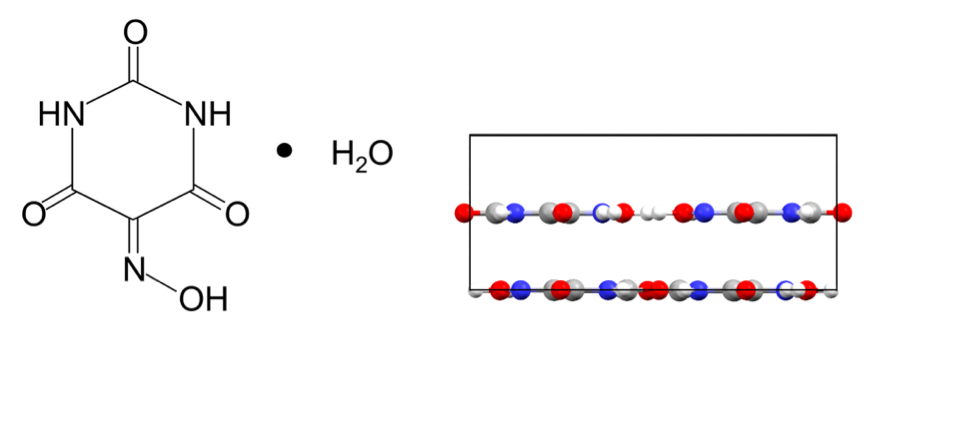
\includegraphics[width=1\linewidth]{src/figures/VAMH_figures/VAMH_fig1.png}
  \caption{A) Violuric acid monohydrate (VAMH) molecular structure and B) \textit{Cmc}2\textsubscript{1} crystal configuration. Viewed along c-axis.}
  \label{fig:vamh_fig}
\end{figure}

In a previous study we explored a proposed polymorphic phase transition of barbituric acid dihydrate, a structurally similar compound to VAMH. We concluded through experimental and computational analyses that the reported temperature-dependent phase transition was actually a result of thermal-induced crystal dynamic disorder and a relationship between a high-temperature disordered state and a low-temperature static state, both of which maintained the same crystal symmetry. The proposed phase transition occurred around 217 K, with the molecules shifting from a planar (\textit{Pnma}) to non-planar configuration (\textit{P}2\textsubscript{1}/n) as the temperature of the system was decreased \citep{nichol_btadh_2005,Jeffrey1961,Al-Karaghouli}. Our data was consistent with a dynamic crystal disorder resulting from the oscillation of two non-merohedrally twinned \textit{P}2\textsubscript{1}/n configurations. This oscillation was observed as a planar configuration by X-ray crystallography due to the average of the two energetically equivalent and closely spaced \textit{P}2\textsubscript{1}/n states. Due to the structural similarity between BTADH and VAMH, the accuracy of the VAMH planar \textit{Cmc}2\textsubscript{1}crystal structure was called into question \citep{paul_true_2019}.
Investigation into the crystal conformation of VAMH at 150 K concluded with a redetermination of the space group from planar \textit{Cmc}2\textsubscript{1}to non-planar \textit{Pca}2\textsubscript{1}. Initial normal-mode calculations of the \textit{Cmc}2\textsubscript{1}unit cell resulted in an imaginary mode. Relaxed symmetry geometry optimizations with the initial \textit{Cmc}2\textsubscript{1}unit cell parameters resulted in the perceived Z=2 unit cell with \textit{P}2\textsubscript{1} symmetry. Upon further analysis via THz spectrometry it was discovered that the simulated \textit{P}2\textsubscript{1} and experimental spectra showed poor agreement, with the number of calculated low-frequency phonon modes falling short of those observed experimentally. A final geometry optimization of a 2x2x2 supercell with \textit{P}\textsubscript{1} symmetry yielded a \textit{Pca}2\textsubscript{1} space group (Z=8). The simulated \textit{Pca}2\textsubscript{1} and experimental THz spectra displayed good alignment, concluding that the redetermined crystal structure of VAMH is of \textit{Pca}2\textsubscript{1} symmetry. 

\section{Materials and Methods}
\subsection{Experimental THz Measurements}
Samples were prepared for terahertz spectroscopy measurements by initially grinding a 2.5\% w/w mixture of violuric acid with polytetrafluoroethylene (PTFE) in order to homogenize the samples and reduce particle size in order to minimize scattering effects. The sample-PTFE mixture was then pressed into a free-standing 13mm diameter pellet using a hydraulic pellet press (Specac Ltd., UK), yielding an 888.34 mg pellet with a thickness of 3.03mm. A second pellet using only PTFE was used as a standard reference, with the same dimensions as the sample-containing pellet. The pellets were mounted in a closed-cycle liquid helium cryostat (Crycocool Industries, USA), which permitted variable temperature acquisition between 20 and 300 K. For the terahertz time-domain spectroscopy measurements, a commercial THz-TDS system (Toptica Photonics AG, DE) was used, which consists of a pair of fiber-coupled emitter and receiver modules. Four off-axis parabolic mirrors were used to collimate and focus the terahertz radiation, and the entire spectrometer was continuously purged with nitrogen gas to minimize absorption from atmospheric water vapor. At each temperature, 20,000 terahertz time-domain waveforms were averaged for both the sample and blank, which was repeated four times. The time-domain data were Fourier transformed to obtain terahertz power spectra, and each sample-blank pair was used to produce absorption spectra, with four absorption spectra per temperature averaged to yield the final spectra presented. 
\subsection{Solid-State Density Functional Theory}
The Crystal17 software package was utilized to perform all DFT calculations, using the PBE-D3 functional and pob-TZVP \citep{Peintinger2013} basis set combination \citep{Dovesi2017,Dovesi2014}. Default values were used for the three-body (D3) empirical energy correction for London-type dispersion forces \citep{Dovesi2017,Grimme2010,Grimme2011,Grimme2016}. Atom-only geometry optimizations were run on VAMH confined to the \textit{Cmc}2\textsubscript{1}space group. Initial lattice dimensions and atomic coordinates for this optimization were obtained from the Cambridge Crystallographic Database \cite{nichol_violuric_2005,groom_cambridge_2016}. Space group perceptions were performed using the Avogadro software package with atom position tolerances of 0.01 Å or less \citep{avogadro}. Constant volume geometry optimizations were performed with energy convergence criteria of \(\Delta\)E < 10-6 hartree for initial optimizations and \(\Delta\)E < 10\textsuperscript{-8} hartree for geometry optimizations used for frequency calculations. Normal mode calculations were run for the optimized structures using the total energy convergence criteria of \(\Delta\)E < 10\textsuperscript{-11} hartree. The optimal sampling rate for the k points used to defined the real space density matrix and the reciprocal space Monkhorst grid were determined for the total energy convergence of \(\Delta\)E < 10\textsuperscript{-11} hartree for the \textit{Cmc}2\textsubscript{1}optimization \citep{Gilat1972,monkhorst}. Shrinking factors of 6 were used for all calculations in order to meet the above listed energy convergence criteria. The radial and angular distributions of points were defined by a pruned (75,974) integration grid for each calculation. The truncation tolerances for the Coulomb and HF exchange integral series were set to 10\textsuperscript{-8}, 10\textsuperscript{-8}, 10\textsuperscript{-8}, 10\textsuperscript{-8}, and 10\textsuperscript{-16} hartree. The IR intensities for the normal mode calculations were determined by the Berry phase approach of calculating polarization differences between equilibrium and distorted geometries utilizing the dipole moment derivatives (d\(\mu\)/dQ) \citep{pascale_calculation_2004, Kudin2007,Wu1993}.

\section{Results and Discussion}
\par Initial geometry optimizations of VAMH were performed with the molecules confined to \textit{Cmc}2\textsubscript{1}symmetry group with fixed lattice parameters corresponding to the experimental X-ray crystal structure determined at 150 K (a = 6.0754 Å, b = 14.3430 Å, c = 7.5288 Å, Z = 4). The atomic coordinates from the \textit{Cmc}2\textsubscript{1}cell optimizations were used in a normal mode caluclation for VAMH, resulting in a single imaginary mode at -22.33 cm\textsuperscript{-1}. The potential energy surface following the imaginary mode displacements were scanned, resulting in a double-well potential, with a small energy barrier of 0.058 kJ mol\textsuperscript{-1} between the two energetically equivalent minima (\autoref{fig:vamh_doublewell}). Graphical representations of the displacement vectors for the imaginary mode were constructed to view the molecular displacements associated with the imaginary mode (\autoref{fig:vamh_imaginarymode}). As seen, the atomic displacements were observed to be equal, but opposite across the vertical mirror plane (parallel to the b-c plane) within the molecule, suggesting an in-phase rocking motion between two mirrored configurations.

\begin{figure}[htbp]
  \center
  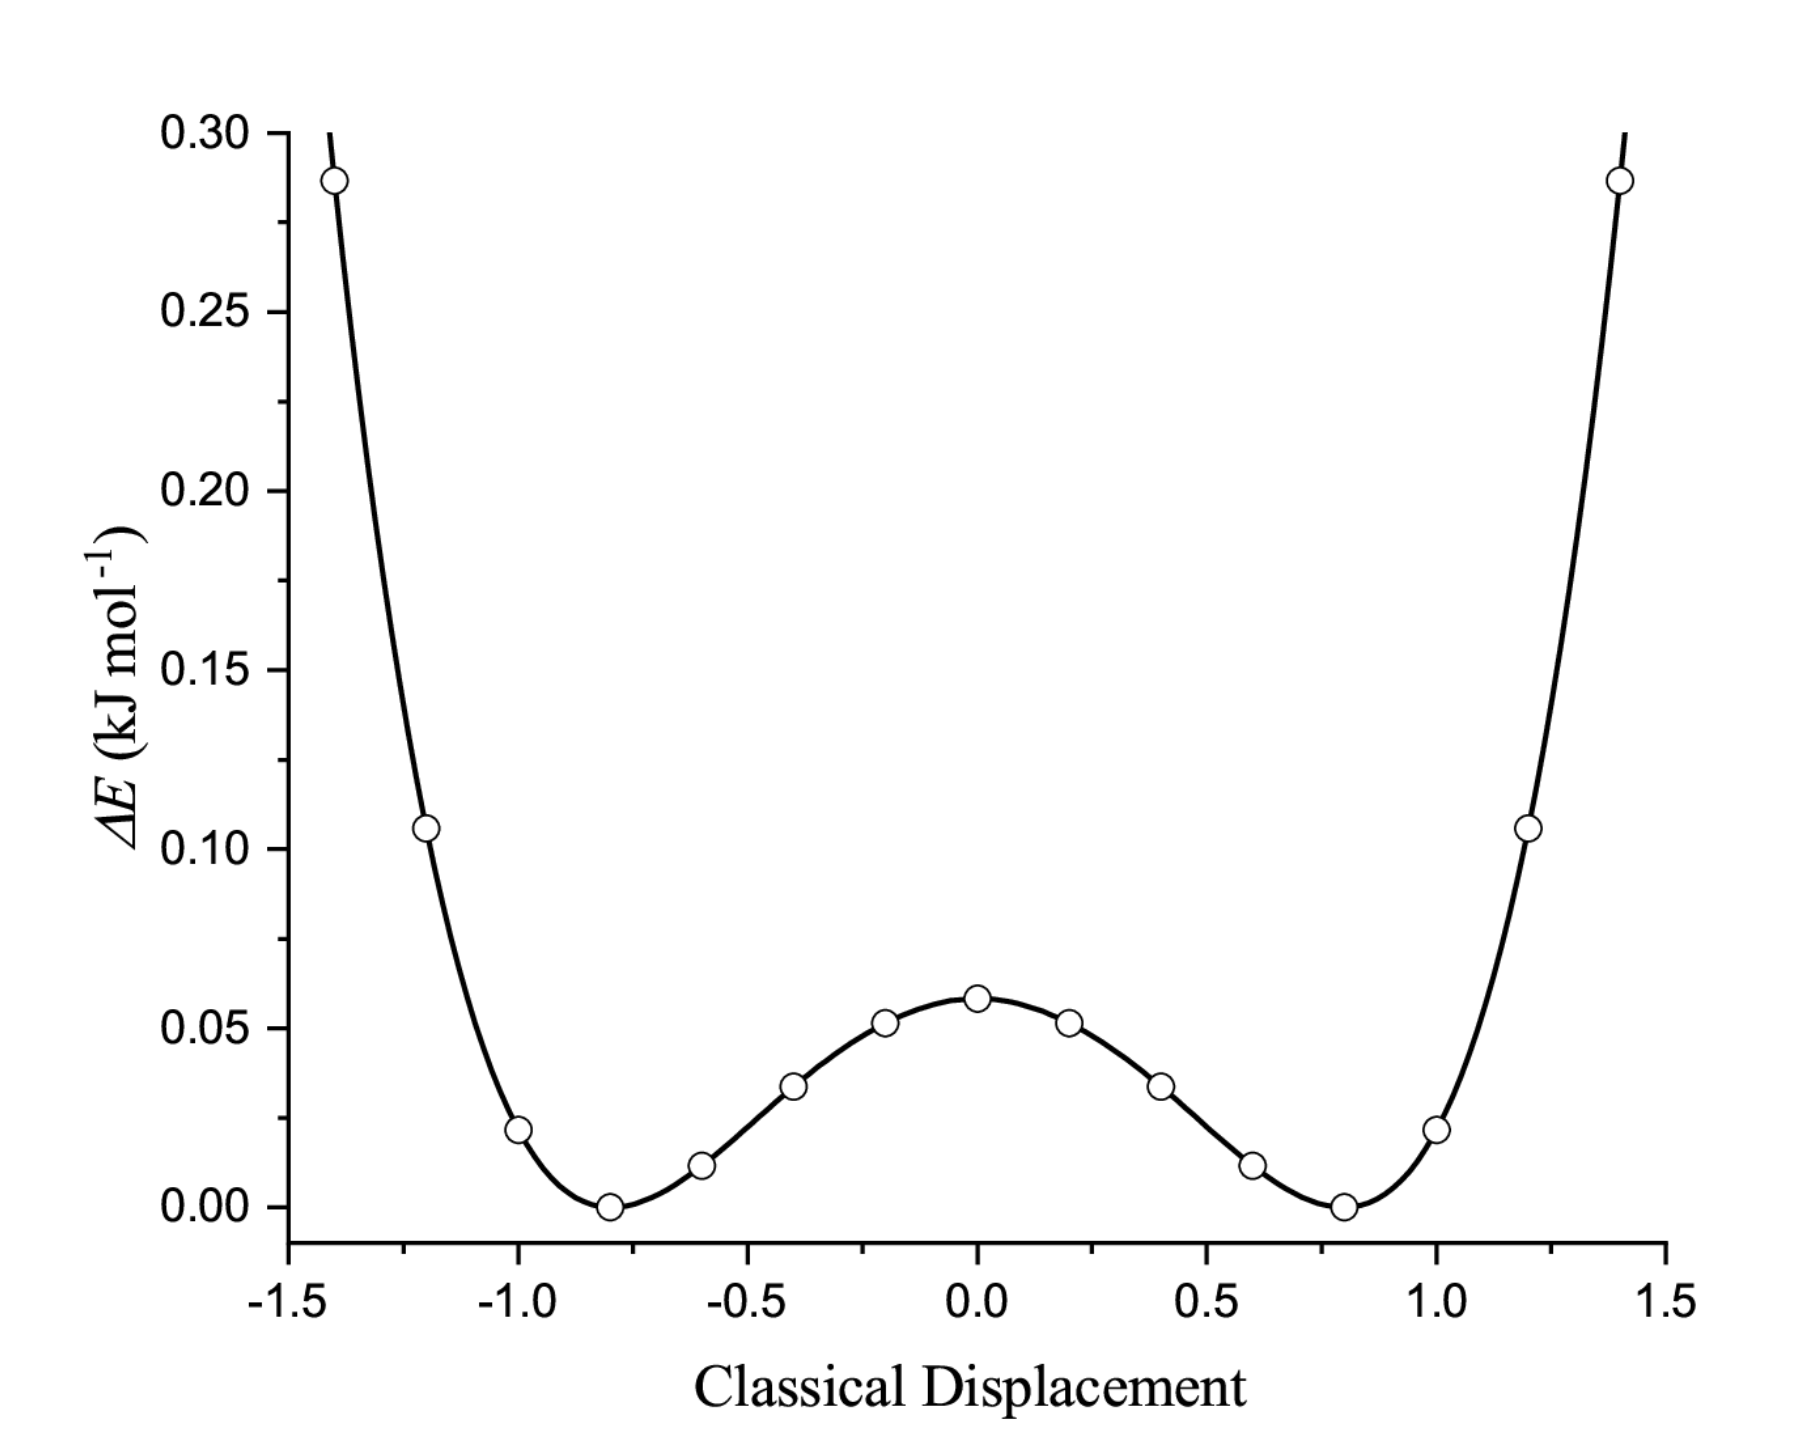
\includegraphics[width=1\linewidth]{src/figures/VAMH_figures/VAMH_potescan.png}
  \caption{Potential energy scan along imaginary mode at 150 K.}
  \label{fig:vamh_doublewell}
\end{figure}

\begin{figure}[ht]
  \center
  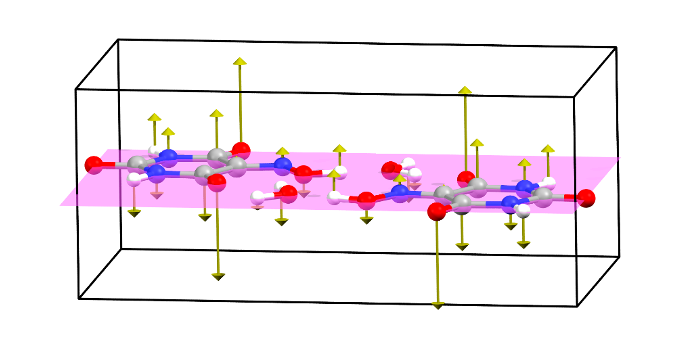
\includegraphics[width=1\linewidth]{src/figures/VAMH_figures/VAMH_fig3.png}
  \caption{A) Vibrational character of the imaginary mode clauclated at 22.33 cm-1 for VAMH constrained to \textit{Cmc}2\textsubscript{1}space group symmetry. Atomic displacement vectors are represented by yellow arrows (magnitudes scaled ×10). }
  \label{fig:vamh_imaginarymode}
\end{figure}

To further investigate the energetically favorable crystalline packing of VAMH, all symmetry constraints were removed, relaxing the \textit{Cmc}2\textsubscript{1}space group to \textit{P}\textsubscript{1}. Constant-volume geometry optimizations were performed at various volumes to investigate the effect of unit cell size (i.e. thermal expansion) on the optimization of the molecules. The lattice parameters and calculated electronic energies of the optimized structures are tabulated in the Supporting Informtion. The molecules in each of the resulting optimized structures were shifted slightly out of plane, as seen in \autoref{fig:vamh_p1andp21} and \autoref{vamh_planes}.  The optimized \textit{P}\textsubscript{1} structure corresponding to the 150-K experimental unit cell volume was analyzed, and a higher-symmetry \textit{P}2\textsubscript{1} molecular configuration was perceived with parameters a = 6.31442 Å, b = 7.31395 Å, c = 7.74019 Å, \(\beta\) = 113.4318°, Z = 2. The \textit{P}2\textsubscript{1} space group contained only two asymmetric units, which is a reduction of half from the original \textit{Cmc}2\textsubscript{1}space group. Subsequent constant volume geometry optimizations with \textit{P}2\textsubscript{1} symmetry were conducted resulting in the b-cell length being reduced by approximately half from the \textit{Cmc}2\textsubscript{1}to \textit{P}2\textsubscript{1} configuration, along with the \(\beta\)-angle increasing from 90° to approximately 113°. An overlay of the \textit{P}\textsubscript{1} (green) and \textit{P}2\textsubscript{1} (black) unit cells within the crystal structure is shown in \autoref{fig:vamh_p1andp21}A. 

\begin{figure}{ht!}
  \center
  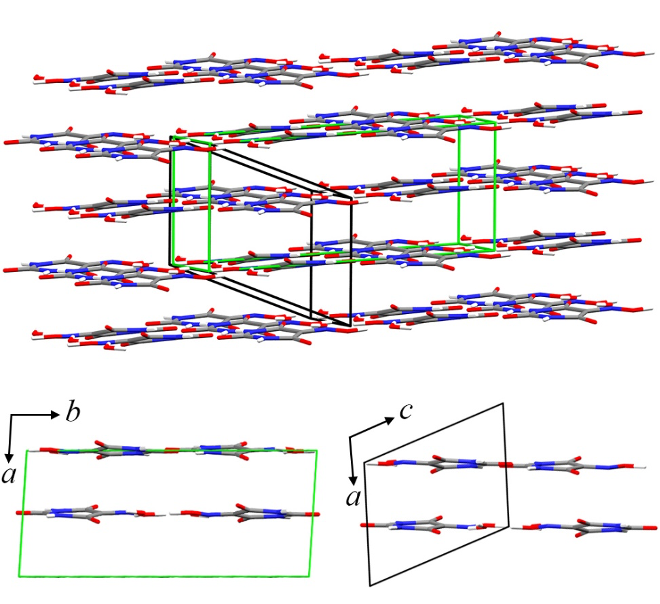
\includegraphics[width=1\linewidth]{src/figures/VAMH_figures/VAMH_fig4.png}
  \caption{A) \textit{P}\textsubscript{1} and \textit{P}2\textsubscript{1} unit cell overlay. B) Packed \textit{P}\textsubscript{1} unit cell viewed along the c axis. C) Packed \textit{P}2\textsubscript{1} unit cell viewed along the b axis.}
  \label{fig:vamh_p1andp21}
\end{figure}

\begin{figure}{ht!}
  \center
  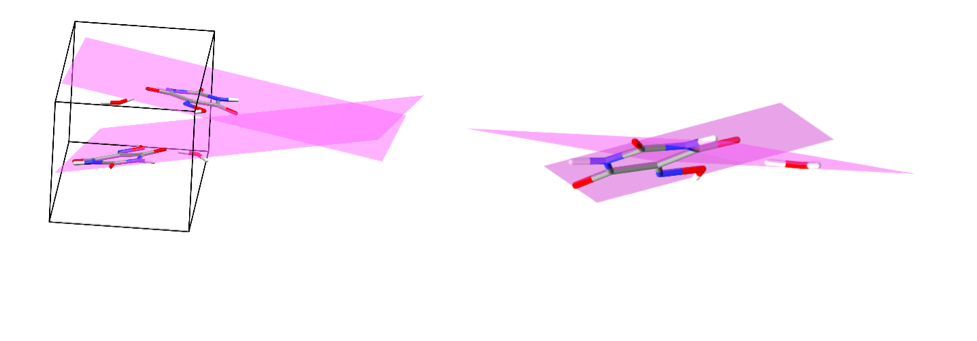
\includegraphics[width=1\linewidth]{src/figures/VAMH_figures/vamh_fig5.png}
  \caption{Depicted planes between A) violuric acid molecules and B) water violuric acid molecular planes of VAMH confined to the \textit{P}2\textsubscript{1} space group.}
  \label{vamh_planes}
\end{figure}


Correlating the static molecular orientations observed in the \textit{P}\textsubscript{1} and \textit{P}2\textsubscript{1} optimized structures with the imaginary mode character obtained from the \textit{Cmc}2\textsubscript{1}normal mode calculations revealed that the out-of-plane molecular shifts correspond to the direction of the imaginary mode displacement vectors shown in \autoref{vamh_planes}. This break in planar symmetry from \textit{Cmc}2\textsubscript{1}to \textit{P}2\textsubscript{1} can be explained by the changes in intermolecular contacts between the two configurations (\autoref{fig:vamh_electrostatic_contacts}, \autoref{tab:vamh_distances}). Relaxation of the crystal symmetry permits the formation of more stable hydrogen bonding and an increased distance of repulsive O···O contacts between adjacent VA molecules (labeled as contact 5). Considerably more favorable direct hydrogen bonding involving the water molecule was obtained in \textit{P}2\textsubscript{1}, most markedly for contact 2 which was reduced by -0.501 Å in comparison to the \textit{Cmc}2\textsubscript{1}structure. Contacts 1 and 4 were modestly reduced by -0.033 and -0.028 Å, respectively. The contact 3 distance remained relatively unchanged between the two crystal structures. Also contributing to the addition stabilization of the \textit{P}2\textsubscript{1} optimized structure is the increase in the short-contact O···O distance between carbonyl oxygens of neighboring VA molecules by 0.048 Å, thereby reducing the repulsive strain forces present within the crystal structure.

\begin{figure}[ht!]
  \center
  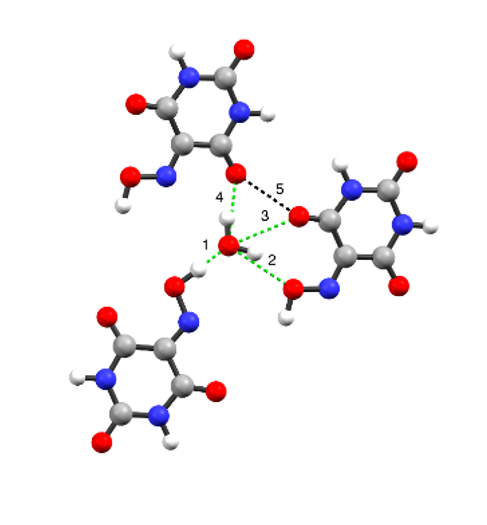
\includegraphics[width=0.7\linewidth]{src/figures/VAMH_figures/VAMH_fig6.png}
  \caption{Primary electrostatic contacts observed in the VAMH crystal structures. Hydrogen bonds are indicated by dashed green lines and repulsive interactions by dashed black lines.}
  \label{fig:vamh_electrostatic_contacts}
\end{figure}

\begin{table}[h]
    \centering
    \caption{Heavy atom distances for intermolecular contacts observed in the \textit{Cmc}2\textsubscript{1}and \textit{P}2\textsubscript{1} optimized unit cells.}
    \begin{tabular}{cccc}
    & \multicolumn{2}{c}{\textbf{Distance (Å)}} & \\
    \textbf{Contact} & \textbf{Cmc2\textsubscript{1}} & \textbf{\textit{P}2\textsubscript{1}} & \textbf{Difference} \\
    \hline
    \textit{1} & 2.507 & 2.474 & -0.033 \\
    \textit{2} & 2.969 & 2.468 & -0.501 \\
    \textit{3} & 2.758 & 2.761 & 0.003 \\
    \textit{4} & 2.676 & 2.648 & -0.028 \\
    \textit{5} & 2.745 & 2.793 & 0.048 \\
    \end{tabular}
    \label{tab:vamh_distances}
\end{table}

In effort to validate the proposed \textit{P}2\textsubscript{1} symmetry configuration of VAHM, the phonon vibrational frequecnies were calculated using the optimized crystal coordinates. As expected, there were no imaginary modes calculated in the normal mode analysis of the \textit{P}2\textsubscript{1} crystal structure, suggesting that a minimum energy configuration was acchieved. The calculated low-frequency vibrational modes were subsequently compared to experiemtnal THz spectrum of VAMH obtained in the spectral range of 10-130 cm-1 (\autoref{vamh_p21_thz}). It was observed that the simulated \textit{P}2\textsubscript{1} THz spectra did not align well with the experimental spectrum, with a notably lower claculated density of states. Only 5 IR-active phonon modes having appreciable absorption intensities were claulcted in the probed spectral range while 9 modes could clearly b resolved in the experimental THz spectrum, along with several evident underlying modes contributing to obsereved peak asymmetry. The additional peaks in the experimental spectrum could not be accounted for with the predicted \textit{P}2\textsubscript{1} crystal structure, however the calculated modes could be tentatively correlated to observed spectral features. This inducated that the basic VAMH molecular orientations predicted in the \textit{P}2\textsubscript{1} configuration were perhaps correct, but the Z=2 unit cell was too reduced and thereby limited the number of phonon modes present in the calculations. 

\begin{figure}[ht!]
  \center
  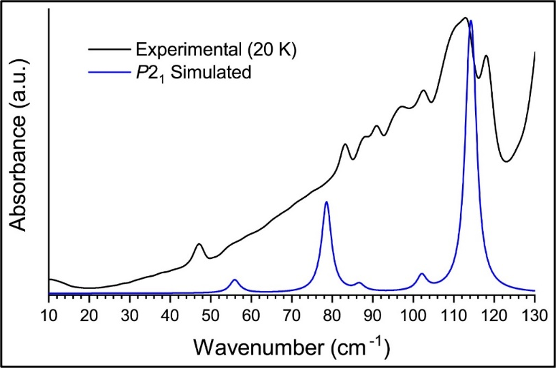
\includegraphics[width=1\linewidth]{src/figures/VAMH_figures/vamh_fig7.png}
  \caption{Comparison of the simulated \textit{P}2\textsubscript{1} THz spectrum to the experimental THz spectrum obtained at 20 K. Lorentzian lineshapes of FWHM 5 cm-1 were convolved into calculated normal modes, and mode intensities of calculated and experimental spectra were normalized.}
  \label{vamh_p21_thz}
\end{figure}

In light of the information provided by the experimental THz spectra, a 2×2×2 supercell was generated from the original \textit{Cmc}2\textsubscript{1}crystal structure, and a geometry optimization was performed with reduced \textit{P}\textsubscript{1} symmetry under constant volume constraints. The resulting structure was then analyzed for symmetry elements present winthin the \textit{P}\textsubscript{1} supercell. Using an atomic-position tolerance of 0.05 Å, a new unit cell of \textit{Pca}2\textsubscript{1} symmetry was percieved to be contained within the optimized \textit{P}\textsubscript{1} supercell structure (\autoref{fig:vamh_pca21}). The VAMH molecular orientations of the larger \textit{Pca}2\textsubscript{1} (Z=8, Z’=2) resembled those observed in the previously predicted \textit{P}2\textsubscript{1} (Z=2, Z’=1) crystal structure. However, the VAMH molecular pairings along the elongated c axis were now related by a screw axis as opposed to restricted translationally invariant in the reduced \textit{P}2\textsubscript{1} packing configuration. The predicted lattice demensions of the \textit{Pca}2\textsubscript{1} and the \textit{P}2\textsubscript{1} crystal structures provided in \autoref{tab:vamh_unitcell_params}. 

\begin{figure}[ht!]
  \center
  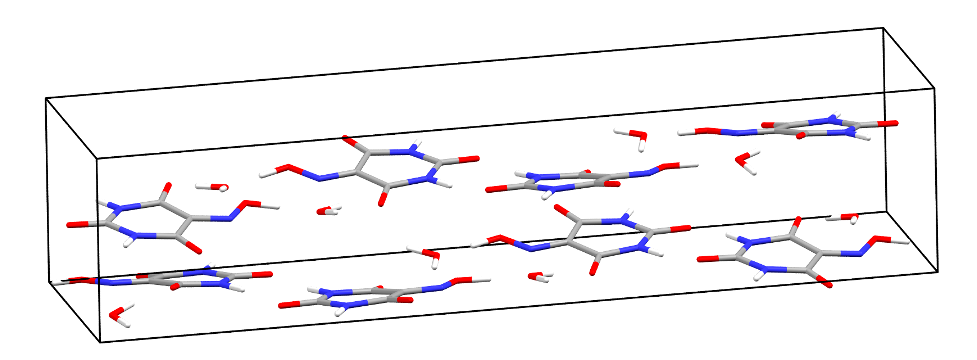
\includegraphics[width=1\linewidth]{src/figures/VAMH_figures/vamh_fig8.png}
  \caption{Molecular packing of the predicted VAMH \textit{Pca}2\textsubscript{1} crystal structure.}
  \label{fig:vamh_pca21}
\end{figure}
  
Comparison of calculated unit cell energies shows the energetic favorability of the \textit{Pca}2\textsubscript{1} unit cell configuration, with relative energy 1.052 kJ mol-1 molecule-1 lower in energy than the \textit{P}2\textsubscript{1} cell and 1.647 kJ mol-1 molecule-1 lower than the constrained \textit{Cmc}2\textsubscript{1}structure (\autoref{tab:vamh_unitcell_params}). The energy difference separating each crystal form is small and presents a low transition barrier between equivalent configurations related by the \textit{Cmc}2\textsubscript{1}reflection planes. The phase coexistence is likely the cause of the apparent crystal disorder and the original conclusion of VAMH residing in the \textit{Cmc}2\textsubscript{1}space group, as this would represent the average of two mirrored equivalent energetic minima. 


\begin{table}[h]
    \centering
    \caption{Tabulated comparison of the unit cell parameters and electronic energies of the investigated symmetry groups.}
    \begin{tabular}{cccccc}
    &&&&& \textbf{Relative Energies} \\
    & \textbf{a (Å)}& \textbf{b (Å)}& \textbf{c (Å)}& \textbf{beta (\textsuperscript{o}) }& \textbf{(kJ mol-1 molecule-1)}\textsuperscript{a}\\
    \hline
    \textsuperscript{b}\textbf{Cmc2\textsubscript{1}} & 6.0754 & 14.3430 & 7.5288 & 90 & 1.647 \\
    \textbf{\textit{P}2\textsubscript{1}}	& 6.31442 & 7.31395 & 7.74019 & 113.4318 & 1.052 \\
    \textbf{\textit{Pca}2\textsubscript{1}} & 7.32092 & 6.31631 & 28.37480 & 90 & 0.000 \\
    \hline
    \multicolumn{6}{l}{\textsuperscript{a}Relative energies obtained from constant-volume optimizations; \textsuperscript{b}Ref \citep{nichol_violuric_2005}.}
    \end{tabular}
    \label{tab:vamh_unitcell_params}
\end{table}

Normal modes of vibration were calculated for the predicted \textit{Pca}2\textsubscript{1} crystal structure and the low-frequency vibrational modes were compared with the experimental THz spectrum (\autoref{fig:vamh_pca21_thz}). A good quality fit of the simulated spectrum to the experimental was obtained. The number of calculated modes is sufficient to assign many of the experimental peaks, with additional low-intensity calculated modes that likely contribute to the high and uneven baseline of the THz spectrum, as well as to the peak asymmetry observed in several of the experimental features. The calculated vibrational frequencies were generally underestimated upon inspection of the spectral comparison. A reasonable explanation for this result is the comparison of the simulated spectrum calculated from an effective 150 K unit cell volume s the structure was optimized under constant-volume conditions from the original \textit{Cmc}2\textsubscript{1}crystal structure measured at this temperature \citep{leguy_dynamic_2016}. The simulated spectrum is overlayed with the experimental spectrum obtained at 20 K for enhanced resolution of experimental spectral features.  
 
\begin{figure}[ht!]
  \center
  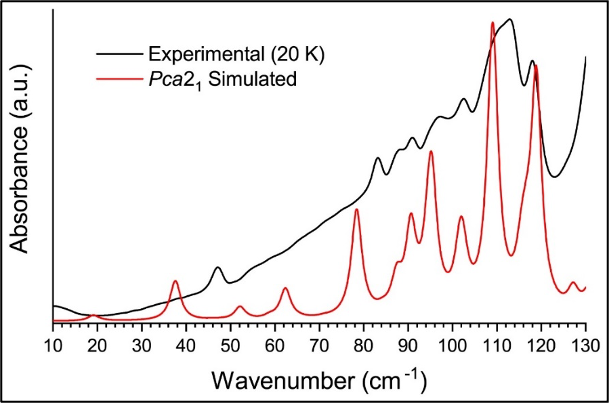
\includegraphics[width=1\linewidth]{src/figures/VAMH_figures/vamh_fig9.png}
  \caption{Comparison of the simulated \textit{Pca}2\textsubscript{1} THz spectrum to the experimental THz spectrum obtained at 20 K. Lorentzian lineshapes of FWHM 5 cm\textsuperscript{-1} were convolved into calculated normal modes, and mode intensities of calculated and experimental spectra were normalized. }
  \label{fig:vamh_pca21_thz}
\end{figure}

Through a systematic computational analysis of the VAMH crystal structure in conjuction with experimental validation by low-frequency THz spectroscopy, a redetermination of the VAMH crystal structure was achieved. The previously reported \textit{Cmc}2\textsubscript{1} crystal structure exhibiting a planar arrangement of violuric acid and water molecules was shown to be inaccurate and likely the result of structural averaging during experimental X-ray measurements. Similar behavior was previously reported for the structurally similar barbituric acid dihydrate, for which a planar configuration  of \textit{Pnma} symmetry was reported for the suspected low-temperature polymorph. However, it was conclusively demonstrated that the crystal structure maintained \textit{P}2\textsubscript{1}/n symmetry, that which was reported as the high-temperature polymorph. In the cases of both VAMH and barbituric acid dihydrate, the planar crystalline configuration represents an averaged structure at the transition point connecting two symmetry-equivalent mirrored unit cell structures. At the two minima, distinct crystal symmetries exist that do not conform to the reflection planes imposed by the \textit{Cmc}2\textsubscript{1}and \textit{Pnma} space groups, respectively. In the present study, a more energetically favorable configuration of \textit{Pca}2\textsubscript{1} was identified for VAMH. The validity of the predicted structure was verified using THz spectroscopy. Normal mode calculations of the optimized \textit{Pca}2\textsubscript{1} crystal structure produced phonon modes that were in good agreement with the experimental THz spectra. 

\section{Conclusion}
Investigation into the crystal structure of VAMH demostrated the theoretical and experimetal data did not support the proposed \textit{Cmc}2\textsubscript{1}symmetry configuration. Imaginary modes were observed across a broad range of defined unit cell volumes while VAMH was confined to the planar \textit{Cmc}2\textsubscript{1}configuration. Initial geometry optimizations with all symmetry operations removed resulted in a perceived Z=2 unit cell of space group \textit{P}2\textsubscript{1}. The shift in molecular orientation was supported by the plotting of the displacement vectors along the observed imaginary mode. This information supported that the actual crystalline arrangement of VAMH deviated from the planar configuration, and that the planar structure may be the averaged structure connecting two energetically equivalent non-planer structures. Explained by the double-well potential and imaginary modes revealed with VAMH confined to the \textit{Cmc}2\textsubscript{1}space group. However, when the simulated THz spectrum of the \textit{P}2\textsubscript{1} unit cell was compared to the experimentally obtained spectrum, there was poor agreement between the two. Further evaluation of the original crystal structure yielded an orthorhomic \textit{Pca}2\textsubscript{1} space group configuration following the generation and structural optimization of a 2x2x2 supercell (Z=32) in \textit{P}\textsubscript{1} symmetry. The normal-mode calculation for the \textit{Pca}2\textsubscript{1} unit cell resulted in no imaginary modes and nearly harmonic potentials for the low-frequency phonon modes. When comparing the simulated \textit{Pca}2\textsubscript{1} and experimental THz spectra, there was good alignment between theory and experiment. This study provides a conclusive redetermination of the violuric acid monohydrate crystal structure in \textit{Pca}2\textsubscript{1} symmetry.

%------------------------------------------------------------------------------
\chapter{Validating structural predictions of conjugated macromolecules in Espaloma-enabled reproducible workflows}
The following chapter contains yet to be published work written by me with the guidance of Dr. Eric Jankowski. The following work has been submitted to the International Journal of Molecular Sciences and is expected to be published in Januaray 2025.
\label{chap:EspVal}

\section{Abstract}
We incorporate \texttt{Espaloma} forcefield parameterization into  \texttt{MoSDeF} tools for performing molecular dynamics simulations of organic molecules with \texttt{HOOMD-Blue}. 
We compare equilibrium morphologies predicted for perylene and poly-3-hexylthiophene (P3HT) with the \espff~forcefield in the present work against prior work using the \texttt{OPLS-UA} forcefield. 
We find that after resolving chemical ambiguities in molecular topologies, \espff~is similar to \texttt{GAFF}.
We observe clustering/melting phase behavior to be similar between \espff~and \oplsff, but that the base energy unit of \oplsff~better connects to experimentally-measured transition temperatures.
Short-range ordering measured by radial distribution functions is essentially identical between the two forcefields, and long-range ordering measured by grazing incidence x-ray scattering is qualitatively similar, with \espff~matching experiments better than \oplsff.
We conclude that \texttt{Espaloma} offers promise in the automated screening of molecules from more complex chemical spaces.
%%%%%%%%%%%%%%%%%%%%%%%%%%%%%%%%%%%%%%%%%%%%%%%%%%%%%%%%%%%%%%%%
\section{Introduction}
Molecular simulations offer promise for the high-throughput screening of thermodynamically stable structures from families of molecules.
Such screening studies can identify chemistries and conditions where self-assembly of desired structures are optimized, and can provide insight into identifying chemistry-structure-property relationships that are otherwise inaccessible with experimental methods\cite{daglar_opportunities_2020,liu2018molecular,lin2020review,afzal2020high,meier2004combinatorial,quach2022high}.
One challenge of screening studies, particularly of polymers, is that the parameters that define the interactions between and within model molecules may not have been defined for a given ``off-the-shelf'' forcefield\cite{wang_end--end_2022}. 
In molecular mechanics simulations, forcefields define the potential energies and therefore forces of bond, angle, torsion/dihedral, and non-bonded models of interatomic interactions\cite{hopfinger1984molecular,vanommeslaeghe2014molecular}. 
For example, the popular Optimized Potentials for Liquid Simulations (OPLS) forcefield has mainly been built around simulating hydrocarbons and proteins \citep{opls,ghahremanpour_refinement_2022}.
The General Amber forcefield (GAFF) is optimized for small organic molecules\cite{wang2004development}.

An example of missing parameters arises when attempting to simulate the popular organic semiconductor poly(3-hexylthiophene) (P3HT).
When using OPLS, we find the forcefield is missing parameter definitions for hydrogen-carbon-carbon-sulfur (H-C-C-S) dihedrals. 
In such cases, the simulator typically has had two options: (1) they might reuse a similar parameterization from a forcefield based on their chemical intuition, or (2) they can perform quantum chemical calculations to identify new forcefield parameters\cite{hopfinger1984molecular} that best fit the calculated potential energies.
The former option has the downside of missing important physics and giving inaccurate results, while the latter option requires additional software fluency and calculation time\cite{wang_end--end_2022}.
Both options suffer from an additional shortcoming: the forcefields that result are \textit{different} from the forcefields from which they were derived, which complicates data provenance and reproducibility.

Recent efforts towards making simulations more transparent, reproducible, usable, and extensible (TRUE)\cite{thompson2020towards,jankowski2020perspective} have identified programmatic workflows as a best practice.
In the present context, this means that simulation scripts that fully specify forcefields contribute to more reproducible simulations, even if the forcefields are custom derivatives of prior work\cite{Klein_foyer}.
Quantum chemical calculations could therefore be included into the programmatic specification of custom forcefields and in principle be shared as reproducible workflows.

However, re-running quantum chemical calculations itself introduces software dependency issues and extended runtimes that are redundant.
A new tool that ameliorates this problem is \esp, which is an open-source package that uses graph neural networks to perceive chemical environments in a molecular graph and predict molecular mechanics forcefield parameters \citep{wang_end--end_2022}. 
\texttt{Espaloma} was designed for the investigation of biopolymers and has been used to accurately simulate them \citep{shirts2023, takaba_machine-learned_2024}. 
Of central importance to the present work is \esp's promise to programmatically ``fill in'' missing parameters for organic macromolecules and polymers, enabling more TRUE screening studies without extra quantum chemical calculations (Step 3 of \autoref{MD-Diagram}).

Here, we evaluate \esp~for the modeling of highly conjugated macromolecules.  
We generate forcefield parameters using \esp~and compare them to the ``off-the-shelf'' \texttt{OPLS-UA} and \texttt{GAFF} forcefields where possible.
We compare phase diagrams and morphologies from prior work to validate and quantify \esp's predictive capabilities outside its core training set \citep{wang_end--end_2022}. 
A schematic of the MD workflow we implemented in this work is shown in \autoref{MD-Diagram}. 
\begin{figure}
    \centering
    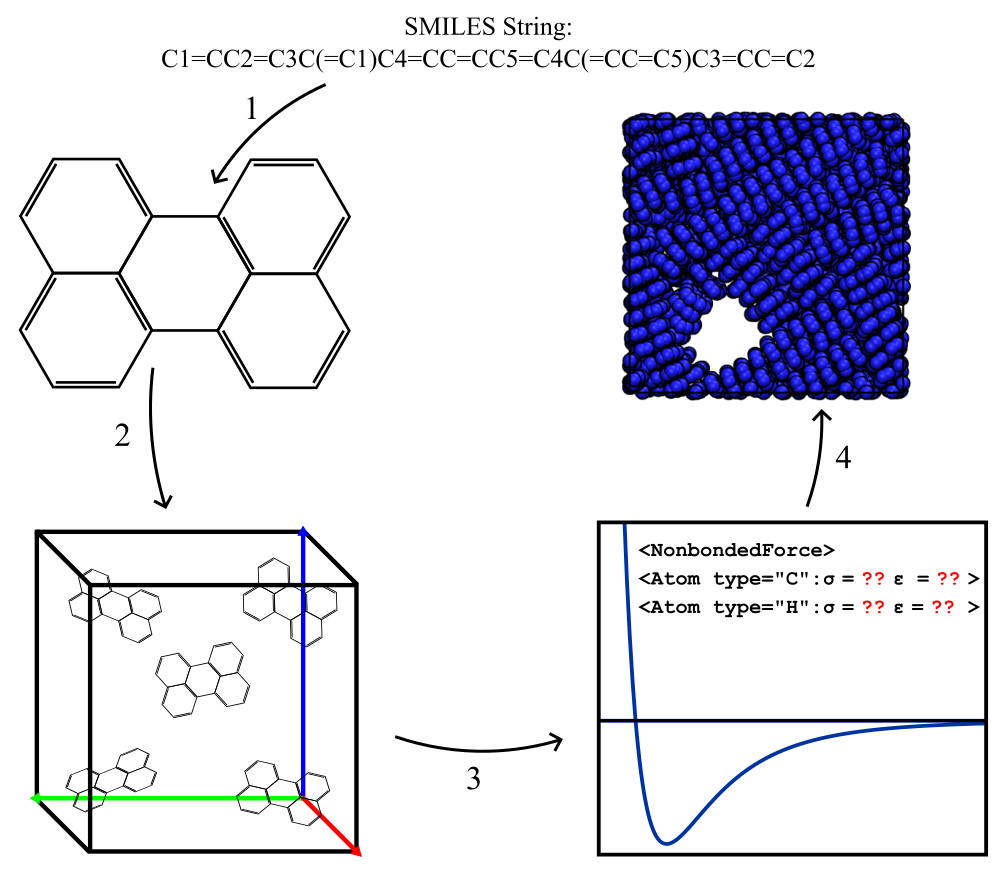
\includegraphics[width=.6\linewidth]{src/figures/FF_figs/MD_process.png}
    \caption{Depictions of our generalized molecular dynamics workflow. Step 1 shows the creation of an \texttt{mBuild Compound} from a SMILES string. In step 2 we create our simulation object using \texttt{flowerMD} and \texttt{PACKMOL}. We employ \esp to parameterize our molecules in step 3 and write the forcefield file. In step 4 we initialize the \texttt{HOOMD-Blue} simulation and predict the morphology of our molecules.}
    \label{MD-Diagram}
\end{figure}


%%%%%%%%%%%%%%%%%%%%%%%%%%%%%%%%%

\section{Model}
We consider united-atom (UA) representations of perylene and P3HT, omitting long-range electrostatics as in prior work\cite{miller_enhanced_2017,miller_optimization_2018}.
Spherical simulation elements are used to represent each ``heavy'' atom and its bonded hydrogens.
Here, the heavy atoms are carbon and sulfur, topologically connected as in \autoref{per_p3ht_fig}.
\begin{figure}[hbt!]
    \centering
    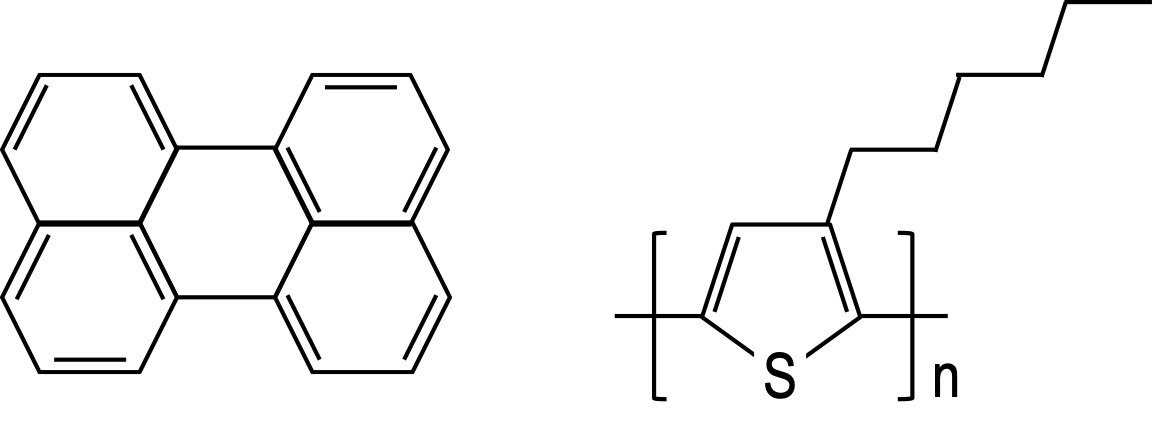
\includegraphics[width=0.6\textwidth]{src/figures/FF_figs/P3HTandPerylene.png} %
    \caption{Diagram of perylene molecule (left) and poly-3-hexylthiophene (P3HT) monomer (right).}
    \label{per_p3ht_fig}
\end{figure}
Chains of $n=15$ repeat units are used to represent P3HT oligomers.
Harmonic potentials are used to model bond-stretching (\autoref{eq:bonds}) and angle bending (\autoref{eq:angles}) between pairs and triplets of bonded atoms. $E_{bonds}$ is the potential energy of a bond, $K_r$ is the bond's harmonic spring constant, $r$ is the internuclear distance, and $r_{eq}$ is the equilibrium internuclear distance. 
\begin{equation}
    E_{bonds} = K_r (r-r_{eq})^2
\label{eq:bonds}
\end{equation}
$E_{angle}$ is the potential energy of a bond angle, $K_{\theta}$ is the harmonic angle constant, $\theta$ is the bond angle, and $\theta_{eq}$ is the equilibrium bond angle. 
\begin{equation}
    E_{angles} = K_{\theta}(\theta-\theta_{eq})^2
\label{eq:angles}
\end{equation}

Cosine series are used to model proper dihedrals (\autoref{eq:dihedrals}) across quadruplets of bonded atoms, where $E_{dihedral}$ is the potential energy of the dihedral, $K_n$ is the force constant of the corresponding particle, $n$, $\phi$ is the dihedral angle, and $\gamma$ is the phase angle. 

\begin{equation}
    E_{dihedral} = \sum_{n=1}^{4}\frac{K_{n}}{2}[1+\cos{(n\phi-\gamma)}]
\label{eq:dihedrals}
\end{equation}

\begin{equation}
    E_{LJ}(r_{i,j}) = 4\epsilon_{i,j} \left[ \left({\frac{\sigma_{i,j}}{r_{i,j}}}\right)^{12} - \left({\frac{\sigma_{i,j}}{r_{i,j}}}\right)^{6} \right] % TODO: This isn't right. Vn aren't defined, nor is gamma, and the LJ potential isn't correct. 
    \label{eq:pairs}
\end{equation}

Simulation elements that are not bonded or separated by more than three bonds within a molecule interact only via the 12-6 Lennard-Jones potential (\autoref{eq:pairs}) \cite{lennard-jones_electronic_1929} truncated at $r_{cut}=2.5\sigma$, where $\sigma$ is the length unit corresponding to the largest simulation element being represented.
Here, this corresponds to sulfur (S) simulation elements for P3HT ($\sigma=3.565$\AA), and carbon (C1) elements for perylene ($\sigma=3.380$\AA).
We apply the Lorentzian combination rule for sigma and a geometric combination rule for epsilon, shown in \autoref{comb_rules}. 
\begin{equation}
    \sigma_{i,j} = \frac{\sigma_{i} + \sigma_{j}}{2}  ,   \epsilon_{i,j} = \sqrt{\epsilon_{i} * \epsilon_{j}}
    \label{comb_rules}
\end{equation}
The parameterization of the bond, angle, dihedral, and nonbonded interaction potentials are generated via \esp~and we describe details and challenges with this in the Methods.

%%%%%%%%%%%%%%%%%%%%%%%%%%%%%%%%%%%%%%%%%%%%%%%%%%

\section{Methods}
In this section we detail the molecular dynamics simulations performed with \texttt{HOOMD-Blue}\cite{anderson_hoomd-blue_2020} to predict equilibrium morphologies, describe the new tools we develop for integrating \esp~into workflows utilize the Molecular Simulation Design Framework (MoSDeF)\cite{cummings2021open}, and detail morphology characterization that underpins model validation.

\subsection{Molecular Dynamics}
Simulations are performed on the Fry high performance computing cluster at Boise State University using \texttt{HOOMD-Blue} on NVIDIA P100 and V100 GPUs. 
We use \texttt{signac}\citep{adorf_simple_2018} to manage simulation workspaces and job submission.
Simulation scripts are available online at \url{github.com/madilynpaul/Espaloma-Validation}. 
Equilibrium morphologies of perylene and P3HT are predicted in the canonical ensemble (constant number of particles $N$, volume $V$, and temperature $T$).
Periodic boundary conditions of cubic volumes are used throughout this work.
We initialize our system using \texttt{PACKMOL}\cite{martinez_p_2009} within \texttt{flowerMD}\cite{Albooyeh2023} to create initial low-density volumes that are randomized at high $T$ (1653 K for P3HT and 696 K for perylene) and a shrinking simulation runs for $5 \times 10^6$ time steps to the target state point density.
Newton's equations of motion are integrated using a two-step MTK velocity-verlet implementation of Nosé-Hoover chains\cite{martyna_constant_1994,cao_adiabatic_1996} with a step size of $dt=0.0003$ for P3HT and $dt=0.0001$ for perylene. 
Simulation volumes are then instantaneously quenched to the statepoint temperature, where the potential energy trajectory is analyzed to determine the onset of equilibrium.
Once the potential energy has stabilized, the simulations continue until decorrelation time measurements provide at least 50 statistically independent snapshots have been generated.

\subsection{Morphology Characterization}
Equilibrium morphologies are quantified using radial distribution functions (RDF) and simulated grazing-incident x-ray scattering (GIXS) implemented in \texttt{freud}\cite{freud2020}.
RDFs are calculated between perylene centers of mass (\autoref{fig:p3ht_per_CG}a), and for P3HT, the sulfur of the thiophene rings (\autoref{fig:p3ht_per_CG}b).
Both the RDF and GIXS analyses are averaged over the last 20 independent snapshots of each simulation.
\begin{figure}
    \centering
    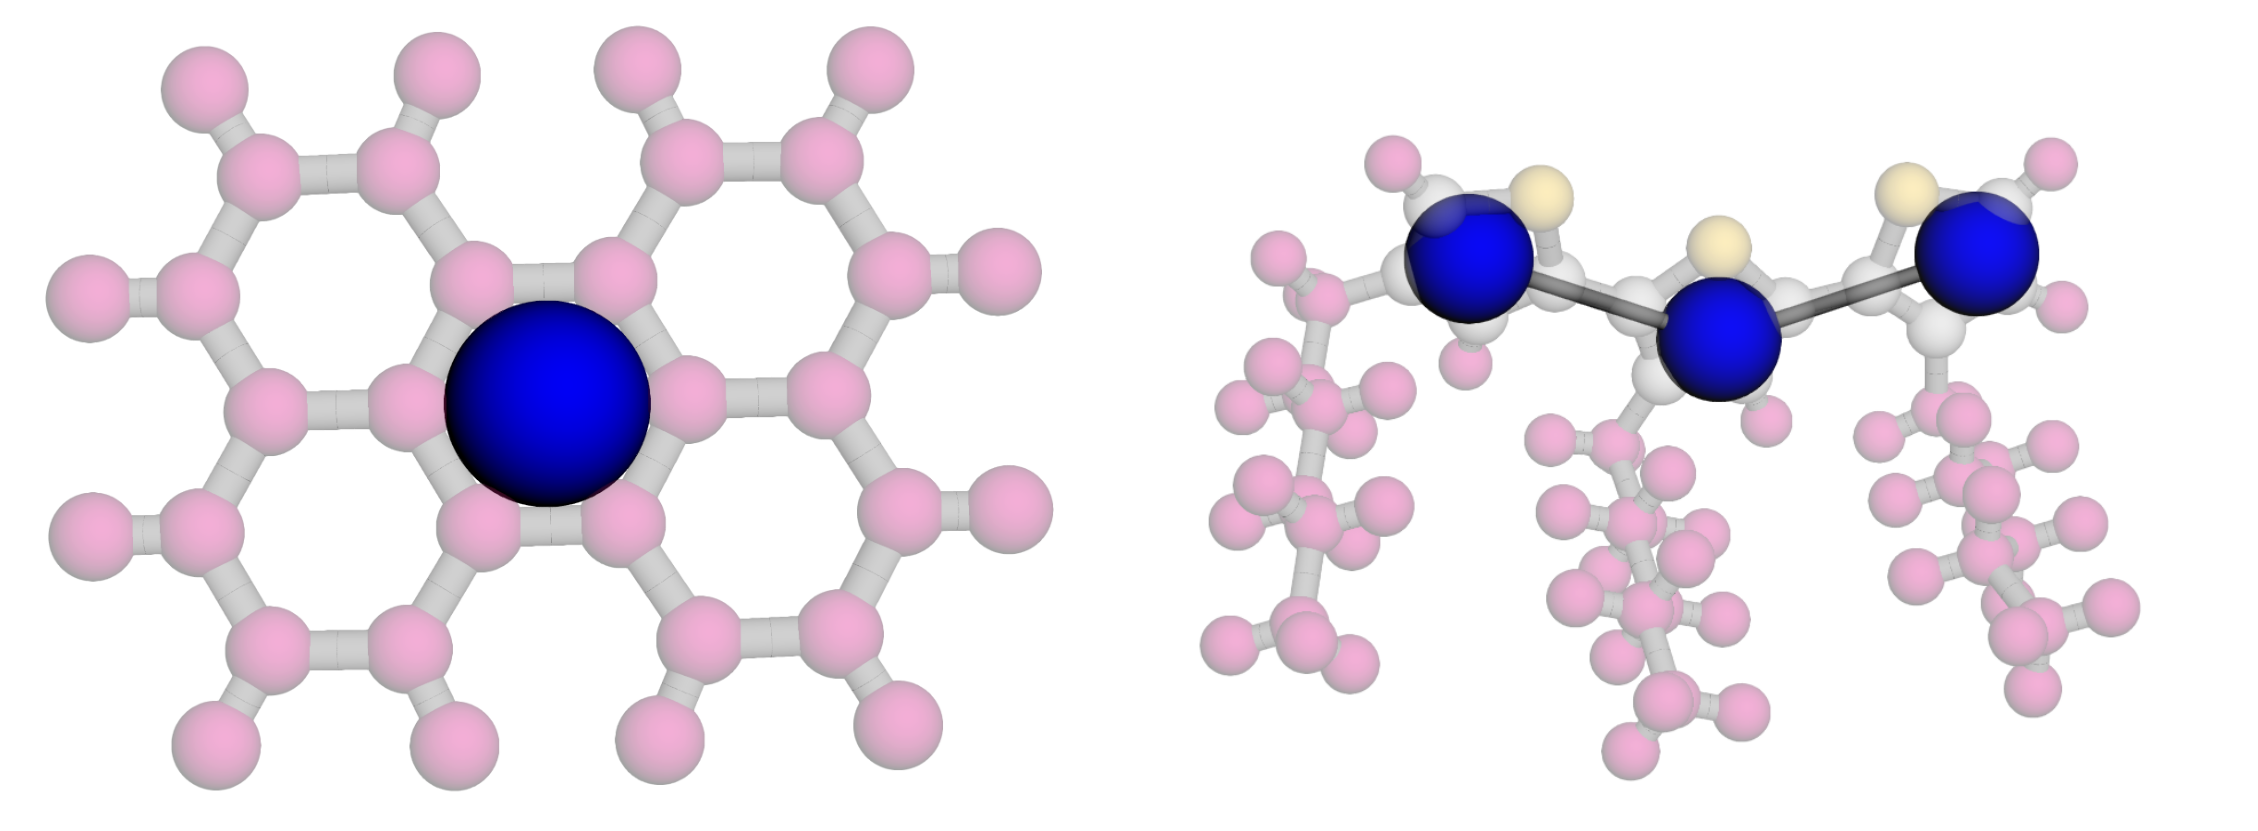
\includegraphics[width=.6\linewidth]{src/figures/FF_figs/per_p3ht_CG.png}
    \caption{Blue spheres represent center-of-geometry positions used for RDFs and clustering criteria. Perylene (left), and P3HT (right).}
    \label{fig:p3ht_per_CG}
\end{figure}

To compare with prior work, we calculate an order parameter $\Psi$ as used by Miller et al.~ \cite{miller_optimization_2018}that measures the fraction of perylene molecules--or monomers for P3HT--belonging to clusters of at least size 6.
Two perylene molecules--or two thiophene rings for P3HT--are considered clustered if their centers are within 6\AA~and the best-fit planes through each moiety are within 10 degrees of being parallel.
The code for calculating RDFs, GIXS, $\Psi$ and phase diagrams is available at \url{github.com/madilynpaul/Espaloma-Validation}. 

\subsection{Integrating Espaloma parameterization into MoSDeF} 

Our simulation workflows are built around MosDeF tools\cite{cummings_opensource_2021}, in particular \texttt{mBuild} \cite{Klein_mbuild} whose \texttt{mbuild Compound} objects are incompatible with the \texttt{openMM Molecule} objects expected by \esp.
To incorporate \esp~into MoSDef workflows we develop a helper function termed ``\texttt{BondWalker}'' that can convert \texttt{mbuild Compounds} into \texttt{openMM Molecules} (\autoref{esp_diagram}).
This workflow fits into the overall MD workflow (Section 4.2, \autoref{MD-Diagram}) within Step 4. 
\begin{figure}
    \centering
    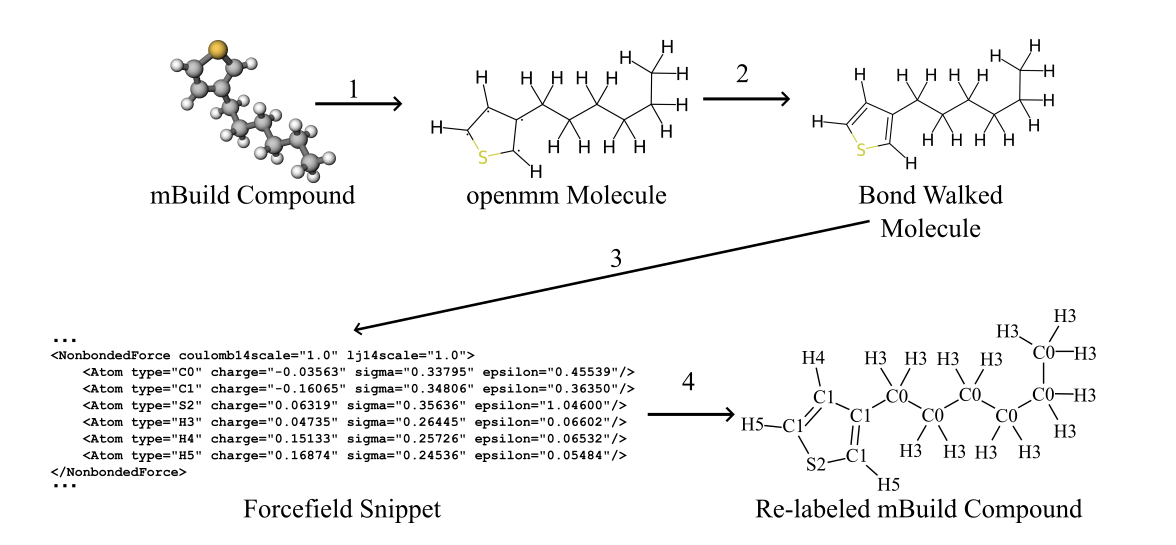
\includegraphics[width=1\linewidth]{src/figures/FF_figs/esp_fig.png}
    \caption{Overall \esp-\texttt{MosDeF} workflow. (1) \texttt{mBuild} compounds are used to create the topology of an \texttt{openMM} molecule, (2) \texttt{BondWalker} uses octet rules to determine double bonds in the \texttt{openMM} molecule. (3) \esp~generates forcefield parameters for the \texttt{openMM} molecule. (4) The \espff~forcefield is used to re-type the \texttt{mBuild} compound for use in \texttt{HOOMD-Blue} simulations.}
    \label{esp_diagram}
\end{figure}
The general procedure is: \textbf{(1)} Create an \texttt{openMM Molecule} topology from connectivity information of the \texttt{mBuild Compound} to be parameterized. 
\textbf{(2)} Rebuild the missing double and triple bonds in the \texttt{openMM Molecule} using the \texttt{BondWalker} function (See \autoref{bond_walk}). 
\textbf{(3)} Pass the \texttt{``BondWalked''} molecule to \esp for forcefield parameterization, writing these parameters to a forcefield \texttt{xml} file.
\textbf{(4)} Use the atom labels given by \esp to rename the atoms in our \texttt{mBuild Compound}. 
This last step ensures that the correct parameters will be applied to the corresponding atoms. 
A full tutorial of \esp~forcefield and typed \texttt{mBuild Compound} generation can be found at \url{github.com/madilynpaul/Espaloma-Validation}. 
%\begin{figure}[ht]
\begin{figure}
    \centering
    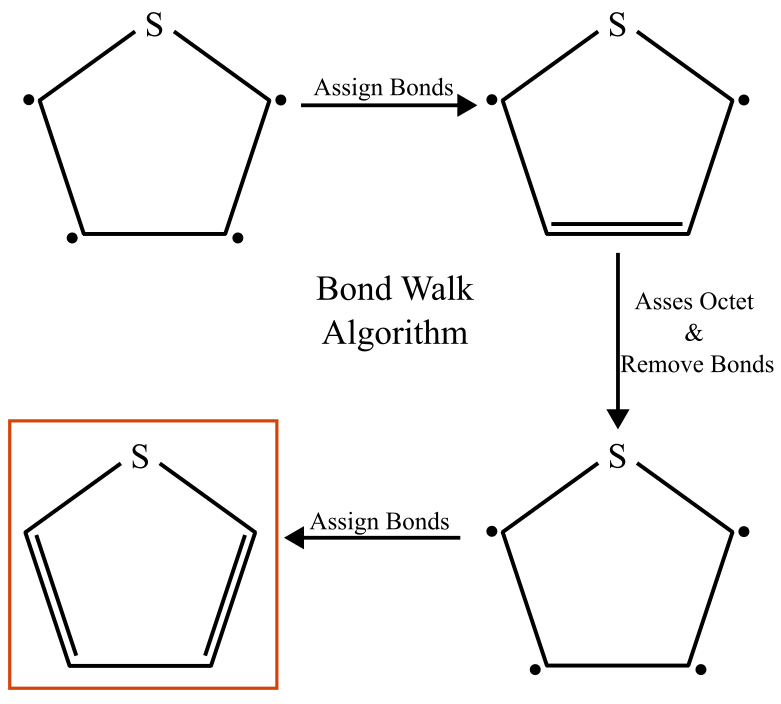
\includegraphics[width=0.5\linewidth]{src/figures/FF_figs/bondwalk_algorithm.png}
    \caption{Double- and triple-bond information that is missing from \texttt{mBuild} compounds is retrieved via \texttt{BondWalker} by iteratively checking whether the octet rules can be satisfied for all atoms after incrementing the bond character adjacent to atoms with unsatisfied octets.
}
    \label{bond_walk}
\end{figure}

%%%%%%%%%%%%%%%%%%%%%%%%%%%%%%%%%%%%%%%%%%%%%%%%%%%%%%

\section{Results and Discussion}
Here we report on the differences between the \espff~, \texttt{GAFF}, and \oplsff~parameters followed by a comparison between \espff~generated morphologies and \oplsff~morphologies generated in prior work.

\subsection{Espaloma vs OPLS-UA and GAFF}
The nonbonded pair interaction for perylene and P3HT are presented in \autoref{sigma_epsilon_comparison_table}, where they are compared against \oplsff~and \texttt{GAFF} parameters. 
\begin{table}[h!]
    \centering
    \caption{Lennard-Jones diameters $\sigma$ and well-depths $\epsilon$ generated by \texttt{espaloma} in the present work, and \texttt{OPLS-UA} and \texttt{GAFF}.}
    \begin{tabular}{c c c c|c c c} 
    & \multicolumn{3}{c}{$\sigma$ (\AA)} &  \multicolumn{3}{c}{$\epsilon$ (kJ/mol)}  \\
    \hline
        &  C1      &   C0      &   S &   C1      &   C0      &   S   \\
    \hline
    \texttt{Espaloma}    &   3.481   &   3.380   &   3.564  & 0.3635  & 0.4554  & 1.046   \\
    \texttt{OPLS-UA}     &   3.436   &   3.905   &   3.436  & 0.4602  & 0.7113  &  1.339   \\
    \texttt{GAFF}        &   3.3997  &   3.3997  &   3.564  & 0.3598  & 0.4577  &    1.046   \\
    \end{tabular}
    \label{sigma_epsilon_comparison_table}
\end{table}
We first consider the LJ $\sigma$ values, and note that \oplsff~is somewhat of an outlier, with much larger C0 diameters, while \espff~and \texttt{GAFF} are similar to each other. 
The \espff~C1's are slightly larger than both \oplsff~and \texttt{GAFF}, while the \espff~C0's are slightly smaller than \texttt{GAFF}.
\texttt{GAFF} and \espff~agree on the diameter of S atoms in P3HT.
We next consider the $\epsilon$ values and note that \espff~is very similar to \texttt{GAFF} once again, with \oplsff~as the outlier.

Normalizing the $\epsilon_{C1}$ and $\epsilon_{C0}$ values by $\epsilon_{S}$ provides a clearer picture of the range of attractions in each model than simple comparison the absolute values of each $\epsilon$.
For \espff, $\epsilon_{C1}/\epsilon_{S}=0.3475$, is nearly identical to that of \oplsff: $\epsilon_{C1}/\epsilon_{S}=0.3437$.
For C0, \espff~$\epsilon_{C0}/\epsilon_{S}=0.4353$, is about 20\% weaker than that of \oplsff: $\epsilon_{C0}/\epsilon_{S}=0.5312$.
To briefly summarize, the C1 parameterizations are close-but-not identical between \espff~and \oplsff, so we expect perylene simulations to be similar between the two models.
However, because the $\epsilon_{C1}/\epsilon_{S}$ and $\epsilon_{C0}/\epsilon_{S}$ ratios and C0 $\sigma$ values vary significantly between \espff~and \oplsff, it is unclear whether P3HT morphologies and phase behavior with \espff~will match those generated previously with \oplsff.

We perform MD simulations of each molecule to compare morphologies generated with the present \espff~parameterization against those previously generated with \oplsff.
A summary of simulation state points and units for each molecule is provided in \autoref{sim_parameters}. 
These statepoints are chosen to replicate structures sampled in prior work from Miller et al.\cite{miller_optimization_2018}.
Each temperature range encompasses the solid-liquid transition temperatures of approximately 500 K and 550 K for P3HT and perylene, respectively. 
The density ranges are chosen with respect to previous MD studies as well as experimental thin-film studies for P3HT\cite{newbloom2012structure}. 
We expect to observe various phases (ordered, liquid, vapor, disordered) over this range of statepoints.

\begin{table}
  \centering
    \caption{A list of statepoints used in the P3HT and perylene simulations, as well as the base units for each simulation (\begin{math}\sigma , \epsilon , M\end{math}).}
  \begin{tabular}{c|c|c}
      & \textbf{P3HT} & \textbf{Perylene} \\
    \hline
    Temperature Range (K) & [60.4,304.4,427.7,608.9]& [49.8,248.8,497.7,746.5]\\
    \hline
    Density Range (g/cm$^3$) & [0.25,0.5,1.0] & [0.5,1.0,1.5]\\
    \hline
    N & 100 & 250 \\
    \hline
    dt & 0.0003 & 0.0001 \\
    \hline
    M (amu) & 32.06 & 12.011 \\
    \hline
    \(\sigma\) (\AA)& 3.56 & 3.40 \\
    \hline
    \(\epsilon\) (kJ/mol)& 1.046 & 0.360\\
    \hline
    N\textsubscript{monomers}& 15 & 1 \\
  \end{tabular}
  \label{sim_parameters}
\end{table}

\subsection{Perylene} %Polish.
The ordering ($\Psi$) of perylene modeled with \espff~ as a function of temperature and density is summarized in \autoref{per_phase_diagram}.
Consistent with Ref.~\citep{miller_optimization_2018}, the most ordered structure (T = 250 K, $\rho$ = 0.5 g/cm$^3$) exhibits significant $\pi$-stacking, which is visible in \autoref{Per_snapshot}. 
At lower temperatures, we observe a transition from highly ordered to less ordered as the density increases, also in agreement with prior work.
This is due to the steric hindrance of having a high number of molecules in a restricted volume is observed in prior work.
\begin{figure}[ht]
    \centering
    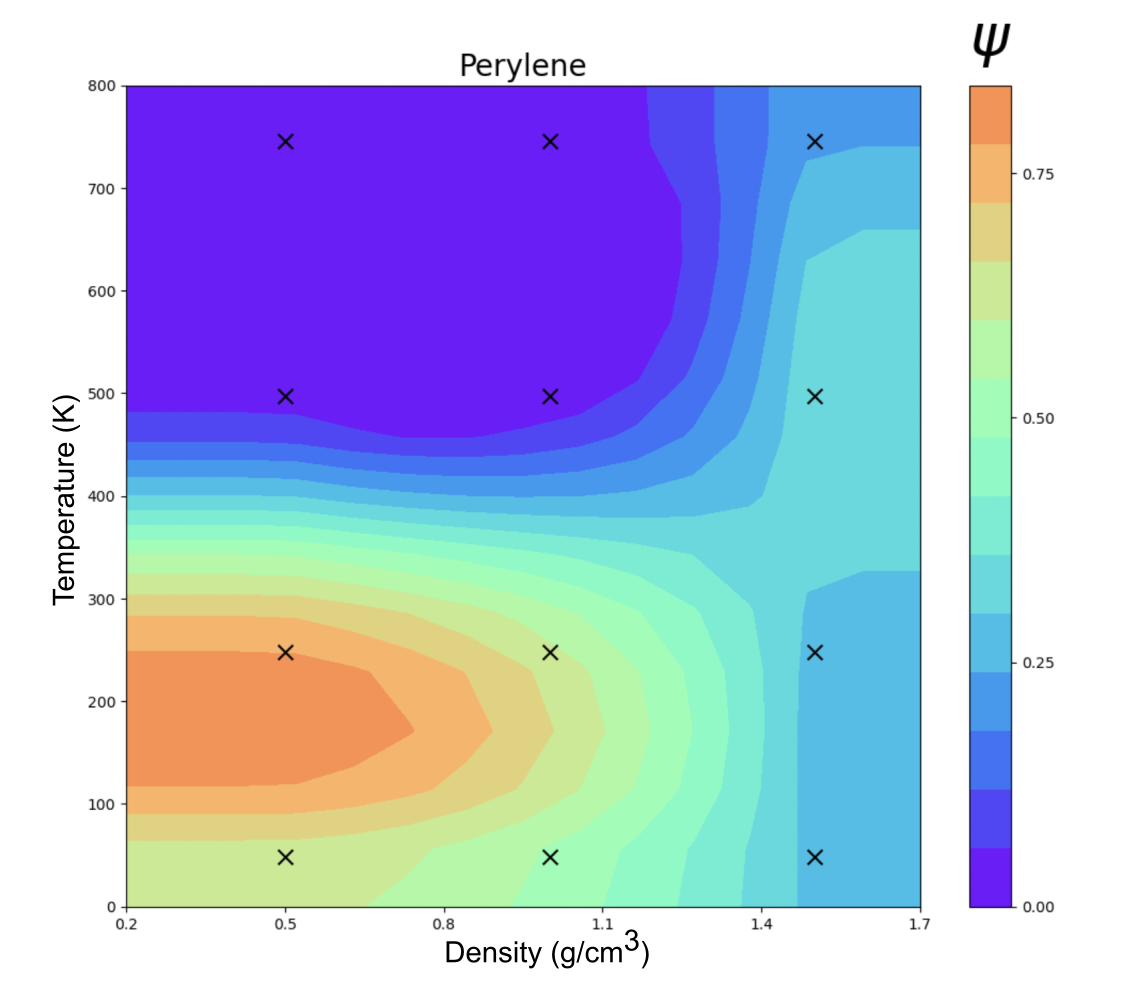
\includegraphics[width=0.6\textwidth]{src/figures/FF_figs/perPD.png} % 
    \caption{Temperature vs density clustering order parameter ($\Psi$) phase diagram of perylene at 12 statepoints.}
    \label{per_phase_diagram}
\end{figure}
\begin{figure}[h!]
    \centering
    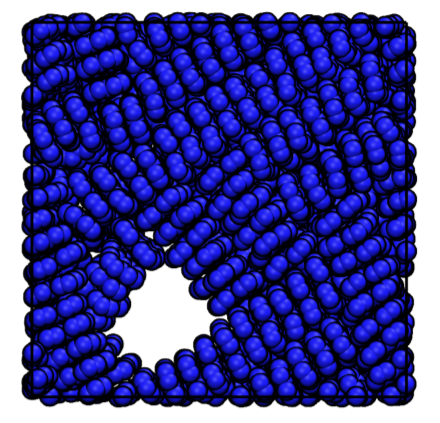
\includegraphics[width=0.35\linewidth]{src/figures/FF_figs/per_snapshot.png}
    \caption{Snapshot of perylene taken from the most ordered morphology at a density of 0.5 g/cm$^3$ and temperature of 248.8 K.}
    \label{Per_snapshot}
\end{figure}
However, the order-disorder transition temperature observed here around 470 K is roughly 0.79 that of the 600 K in Ref.~\citep{miller_enhanced_2017} and Botoshansky et al\cite{botoshansky2003towards}.
This is explained by the difference in base unit between \esp~and \texttt{OPLS-UA} perylene forcefields: Both models have only C1 atomtypes but $\epsilon_{OPLS-UA}=0.4602$ kJ/mol and $\epsilon_{ESP-UA}=0.3635$ kJ/mol. 
The ratio between these two energy units $\frac{\epsilon_{ESP-UA}}{\epsilon_{OPLS-UA}}=0.79$ matches the transition temperature discrepancy.
That is, in dimensionless units, there is no significant difference in the temperature-density phase diagrams between the two forcefields.
Given that the energy unit of \oplsff~gives an order-disorder transition temperature in agreement with experiments, this suggests that the absolute \espff~energy units may benefit from empirical rescaling.

A comparison to the RDFs reported in Miller, et al.~at density of 1.7 g/cm$^3$ and the present work shows good agreement in short-range ordering as a function of temperature.
 First peak locations for the ordered systems in the \espff~and \oplsff~RDF's align at 3.8 \AA. 
 First peak locations in the disordered systems produced by \espff~and \oplsff~both appear at approximately 4 \AA. 
 Differences in peak intensity can be explained by the difference in density between the two systems. 
 As expected, the RDFs calculated  at higher temperatures show less intense peaks. 
 We observe high ordering at 50 K and 249 K, in correspondence to the RDF reported by Miller, et al.~
 We observe consistent RDF peak locations between the \espff~simulation results at temperature of 498 K and the \oplsff~simulation results reported in the droplet phase by Miller, et al.~ 
\begin{figure}[h!]
    \centering
    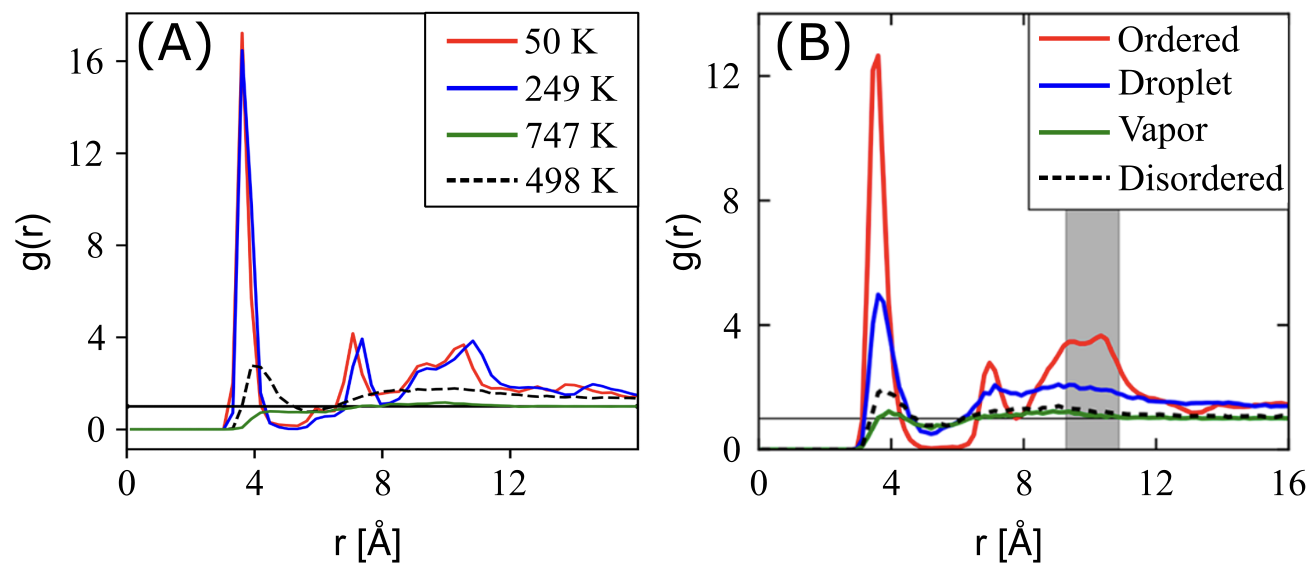
\includegraphics[width=.75\textwidth]{src/figures/FF_figs/per_rdf.png}
    \caption{(A) Radial distribution function (RDF) of Perylene at various temperatures at a density of 0.5g/cm$^3$ generated from an \espff~predicted morphology. (B) RDF of perylene in various phases generated from an \oplsff~predicted morphology. \oplsff~RDF published by Miller, et al.~at Ref \citep{miller_enhanced_2017}.}
    \label{per_rdf}
\end{figure}

Long-range order is measured via simulated GIXS at temperature of 250 K and density of 0.5 g/cm$^3$. 
Bragg reflections are observed along both the x and y axes, indicating significant long-range order and close packed columns, which are observed in \autoref{Per_snapshot}. 
One major difference between the \espff~generated GIXS pattern here and the \oplsff~pattern in prior work is the $q_y$ location of the 001 reflection: From \oplsff~the 001 reflection occurs around $0.8 A^{-1}$, while with \espff~here $q_y=1.9 A^{-1}$ in better agreement with Ishii and Miyasaka\citep{Ishii}.
\begin{figure}[h!]
    \centering
    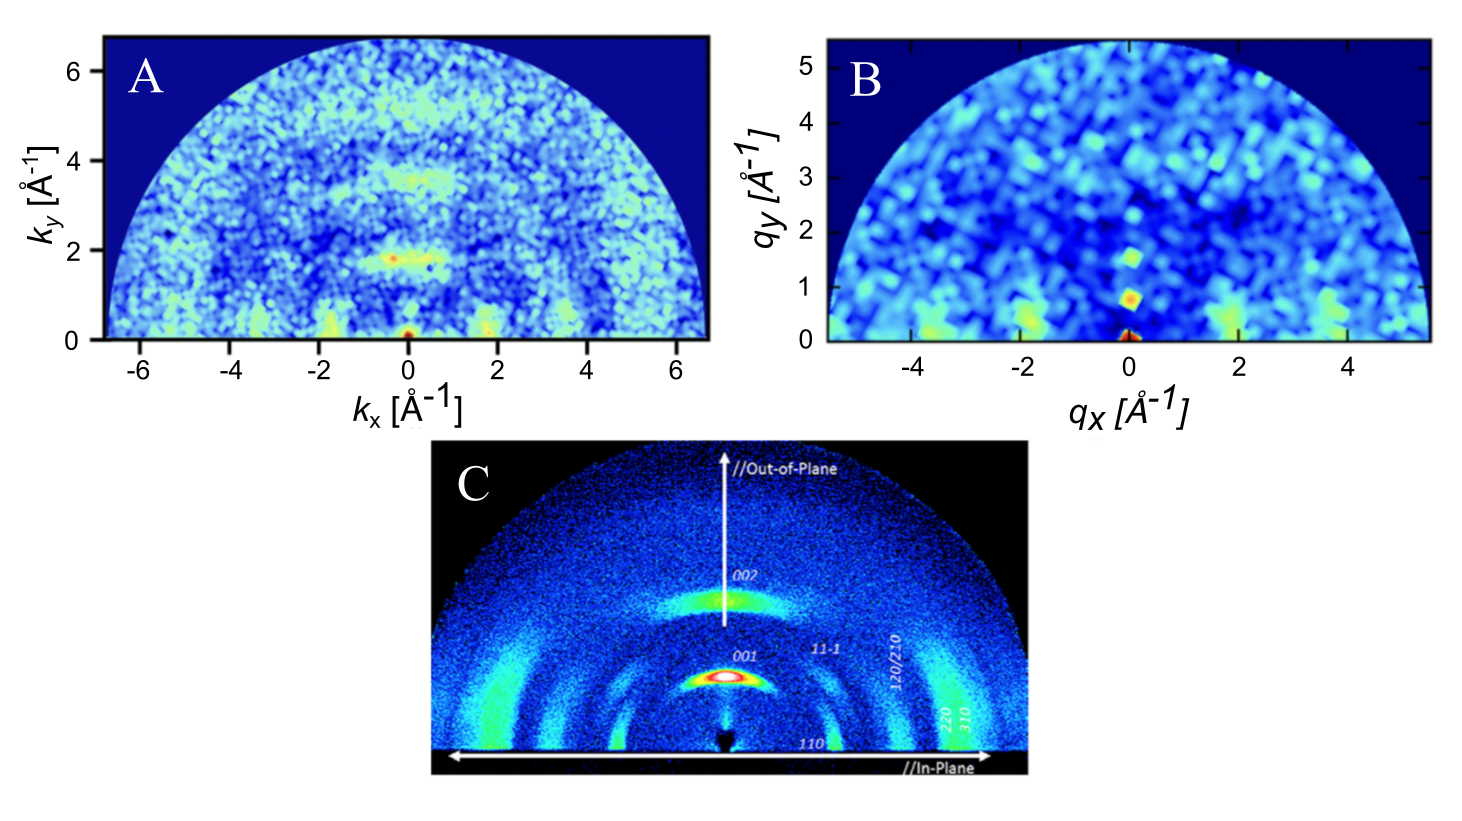
\includegraphics[width=1\textwidth]{src/figures/FF_figs/per_gixs.png} 
    \caption{(A) Grazing incident x-ray scattering pattern of Perylene generated from an \espff~morphology. (B) GIXS pattern of Perylene generated from an \oplsff~morphology. \oplsff~GIXS pattern published by Miller, et. al. at Ref \citep{miller_enhanced_2017}. (C) Experimental XRD pattern for $\beta$-perylene, reproduced with permission from Ishii, et al.~ at Ref \citep{ishii_fully_2014}. Copyright 2014 AIP Publishing LLC.}
    \label{Per_GIXS}
\end{figure}
To briefly summarize, modeling perylene with \espff~parameterization results in phase behavior and short-range ordering in agreement with prior \oplsff~work, however long-range ordering as measured by GIXS matches experiments better, while the base energy unit of \oplsff~gives better temperature correspondence.

%%%%%%%%%%%%%%%%
\subsection{Poly-3-Hexylthiophene (P3HT)}
\begin{figure}[h!]
    \centering
    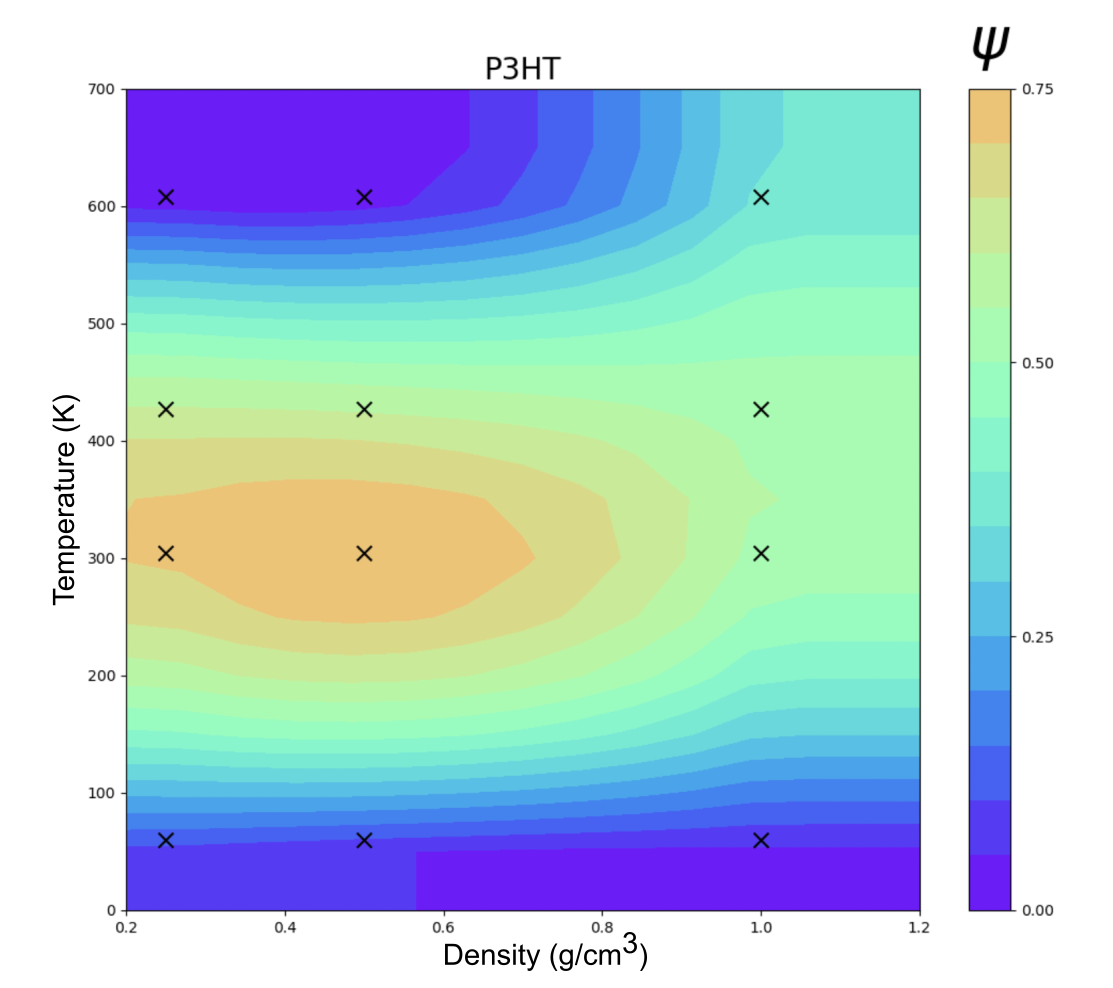
\includegraphics[width=0.6\textwidth]{src/figures/FF_figs/p3htPD.png} % Replace 'example-image' with your image file name and path
    \caption{Temperature vs density clustering order parameter ($\Psi$) phase diagram of P3HT at 12 statepoints.}
    \label{p3ht_phase_diagram}
\end{figure}
\autoref{p3ht_phase_diagram} shows the clustering order parameter ($\Psi$) phase diagram of P3HT as a function of temperature and density. 
 As observed with perylene, the transition temperatures are too low relative to experiments, and this is again explained by the differences in $\epsilon$ units between \espff~and \oplsff.
 \espff~gives an $\epsilon$ of 0.4554 kJ/mol for the aliphatic side chain carbons of P3HT, while \oplsff~uses an $\epsilon$ of 0.7113 kJ/mol. 
 This creates more ordered side chains in the \oplsff~simulations in comparison to the \espff~simulations. 
 This observation is supported by the work in Reference \citep{marsh_controlling_2014}, stating that lower the $\epsilon$ values for side chains of P3HT monomers results in lamellar structures at lower temperatures than if the $\epsilon$ was higher \citep{marsh_controlling_2014}. 
\begin{figure}[h!]
    \centering
    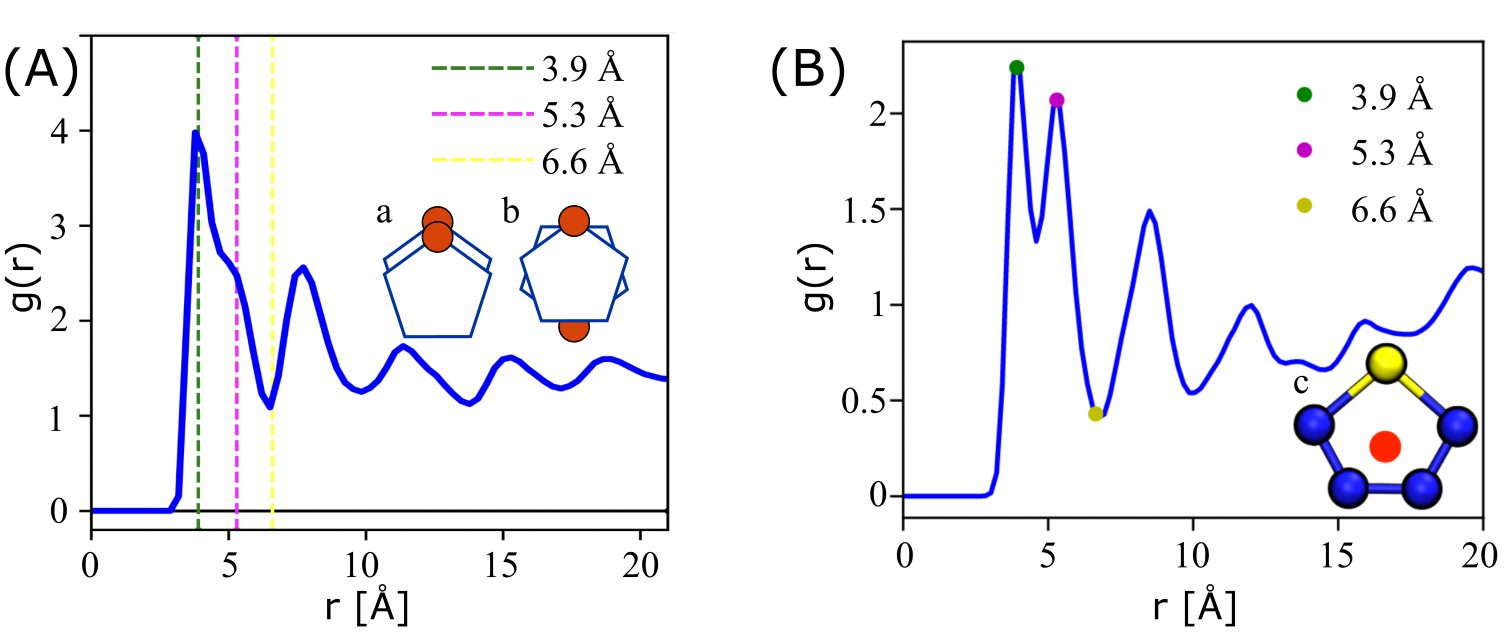
\includegraphics[width=.75\textwidth]{src/figures/FF_figs/p3ht_rdf.png}
    \caption{(A) Radial distribution function (RDF) of P3HT at a temperature of 304 K and a density of 0.5g/cm$^3$ generated from an \espff~predicted morphology. 
 (B) RDF of P3HT generated from an \oplsff~predicted morphology. 
 \oplsff~RDF published by Miller, et al.~in Ref \citep{miller_optimization_2018}.}
    \label{P3HT RDF}
\end{figure}
\autoref{P3HT RDF} shows the radial distribution function of \espff~P3HT (left) and \oplsff~P3HT (right). 
 The \espff~RDF is generated at a temperature of 304 K and a density of 0.5g/cm$^3$. 
 Three vertical dashed lines in the \espff~RDF correspond to the local maxima and minima highlighted in the \oplsff~RDF. 
 The first peak in each corresponds to the aligned $\pi$-stacking of the thiophene rings, shown in \autoref{P3HT RDF}a. 
 The second peak aligns with the anti-aligned $\pi$-stacking of the thiophene rings, shown in \autoref{P3HT RDF}b. 
 The \oplsff~RDF is calculated using the geometric center of thiophene ring, shown in \autoref{P3HT RDF}c. 
 The \espff~RDF is calculated using only the S-S interactions, excluding those in the same chain. 
 The sulfurs were chosen for the \espff~RDF because they are central to the ring, hold the most mass and have the largest radius. 
\begin{figure}[h!]
    \centering
    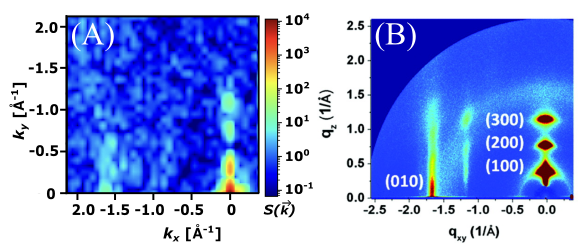
\includegraphics[width=.8\textwidth]{src/figures/FF_figs/p3htGIXS&exp.png}
    \caption{(A) Grazing Incident X-ray Scattering Pattern of P3HT at 0.5 g/$cm^3$ and 304 K generated using \espff. (B) Corresponding experimental scattering pattern of P3HT. Reprinted (adapted) with permission from Ko, et al.~in Ref \citep{p3ht_experimental}. Copyright 2012 American Chemical Society.}
    \label{p3ht_GIXS}
\end{figure}
\par The GIXS scattering pattern of the most ordered structure (0.5 g/cm$^3$, 304 K) displays significant correlation to the experimental scattering pattern of P3HT (\autoref{p3ht_GIXS}). 
 Peaks are observed at approximately 1.65 \AA \textsuperscript{-1} corresponding to the (010) plane, as well as peaks along the (100) plane spaced approximately 0.3 \AA \textsuperscript{-1} apart. 
 This correlation between experiment and simulation confirms that the \espff~is able to responsibly parameterize and represent the P3HT polymer in simulations. 
 The lamellar structure represented by the scattering pattern in \autoref{p3ht_GIXS} is shown in \autoref{p3ht_lamellar}. 
\begin{figure}[hbt!]
    \centering
    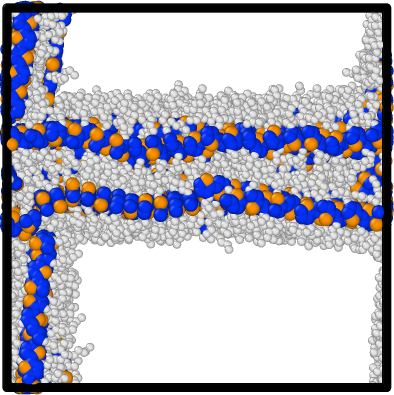
\includegraphics[width=0.5\textwidth]{src/figures/FF_figs/p3ht_0.5den_2.42kT.png}
    \caption{Snapshot of P3HT's most ordered morphology at a density of 0.5 g/cm$^3$ and temperature of 304 K.}
    \label{p3ht_lamellar}
\end{figure}


%%%%%%%%%%%%%%%%%%%%%%%%%%%%%%%%%%%%%%%%%%%%%%%%%

\section{Conclusions}
We successfully incorporate \esp~forcefield generation into \texttt{MoSDeF} workflows for investigating organic molecule phase behavior via MD simulations. 
\esp~generates reasonable forcefield parameters for macromolecules with high aromaticity as well as for thiophene-based conjugated polymers as measured by GIXS, RDF, and phase behavior.
The GIXS scattering patterns for both perylene and P3HT showed long range order that was consistent with published experimental work, and in the case of perylene has better agreement than \oplsff in matching the length scale of the 100 reflection. 
One caveat is that the absolute energy units generated by \espff~may be too low for the molecules of interest.
Here we find that multiplying \espff~$\epsilon$ values by 1.26 to be in closer agreement with \oplsff~gives better agreement for P3HT and Perylene's experimental phase transitions between ordered and disordered phases.
Whether this rescaling rule is universal or is dependent upon the specific chemistries remains the subject of future work.
Nevertheless, the present observations inform confidence in using \esp~to quickly generate forcefields for molecules that are missing information in ``off-the-shelf'' forcefields like \oplsff~and \texttt{GAFF}, subject to the energy-rescaling caveat above.
We conclude that \esp~holds promise as a component in high-throughput screenings of organic molecules for phase behavior in systems from polymer thermoplastics to organic photovoltaics to macromolecular drug packing and more.

%------------------------------------------------------------------------------
\chapter{Temperature dependent chain rigidity study of organic photovoltaic donor-acceptor co-polymers.}
The following chapter contains yet to be published work written by me with the guidance of Dr. Eric Jankowski. 
\label{chap:PersistenceLength}
\section{Summary} 
Donor-acceptor (DA) co-polymers are currently a interesting area of study because of their promise in improving the field of optoelectronics because of their tunable band gaps. Applying these polymers in photovoltaic devices has proven to increase the power conversion efficiency of the device. In this study, we implemented molecular dynamics simulations to investigate the rigidity of complex organic polymers. Utilizing the previously validated workflow (Chapter 4) we built and parameterized 13 conjugated, organic polymers and predicted the bulk morphologies over a large temperature range. From the morphologies we employed a new function to calculated the persistence length $l_p^{MD}$ of each polymer throughout their trajectories. We compare the results to experimental persistence lengths calculated via small angle neutron scattering, $l_p^{SANS}$, and to theoretical results calculated via density functional theory, $l_p^{DFT}$ . We found that for most of the polymers there was good agreements between the $l_p^{MD}$ and $l_p^{SANS}$. From this information we are able to draw conclusions about how differences in side chains and backbone chemistry effects the rigidity of DA co-polymers. 
\section{Introduction}
\begin{wrapfigure}{r}{0.5\textwidth}
    \begin{center}
        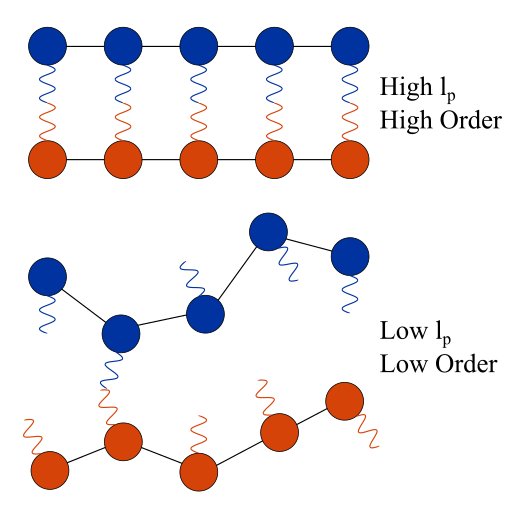
\includegraphics[width=0.48\textwidth]{src/figures/pers_l_figs/persistence_length.png}
    \end{center}    
  \caption{Diagram of how a more rigid polymer (high $l_p$) can lead to higher order in the morphology compared to a more flexible polymer (low $l_p$).}
  \label{pers_length}
\end{wrapfigure}
The morphology that OPV polymers self-assemble into has a significant impact on the power conversion efficiency (PCE) of the solar devices that are made from these materials. Currently,  there is some ambiguity as to why certain morphologies lead to an increase in the PCE as well as what materials might self-assemble into these more efficient morphologies. Drawing connections between the physical and/or chemical properties of polymers to higher efficiency morphologies will enable the discovery of new materials that could increase the PCE of OPV devices. Donor-acceptor (DA) polymers are of a great interest in OPV device design due to their tunable band-gaps and high charge carrier mobilities \citep{sarap_electronic_2023}. DA polymers function as both the electron donor and electron acceptor by alternating electron rich and electron deficient environments. DA polymers are so exciting because we can in theory tune their optoelectronic properties by altering the donors and acceptors as well as their sequencing, all while determining the thermodynamic stability using MD simulations. The persistence length ($l_p$) of a polymer is used to describe the polymer's rigidness, a smaller $l_p$ correlates to a more flexible polymer. The $l_p$ is one measure of both thermodynamic stability as well as a prediction of how well the polymer might order in a bulk morphology. The $l_p$ is a characteristic of polymer chains in a given environment that gives a lot of insight into how the polymer(s) interact and self-assemble into given morphologies. In some cases, the higher the persistence length of a polymer, the higher the observed order of the polymer bulk-morphology will be \citep{martin_temperature-dependence_2018}. Previous studies have found that the straighter a polymer with optoelectronic properties is, the greater the probability of $\pi$-stacking of the backbones, leading to a greater charge carrier mobility in the bulk morphology \citep{Himmelberger_Salleo_2015}. Danielsen et al.~ has drawn a connection between the rigidity of DA copolymers and their molecular structure and side chain size via small angle neutron scattering (SANS). With the abundance of possible donors and acceptors and infinite possible combinations it is impossible to experimentally synthesize and test many DA polymers. Due to this we turn toward molecular dynamics simulations. In this study, we present a computational workflow of modeling and predicting the persistence length of DA polymers. We validate this workflow with 13 OPV polymers by comparing the persistence lengths calculated via MD ($l_p^{MD}$) to those presented by Danielsen, et al.~ using DFT ($l_p^{DFT}$) and SANS ($l_p^{SANS}$). 

\newpage
\begin{figure}[h!]
    \centering
    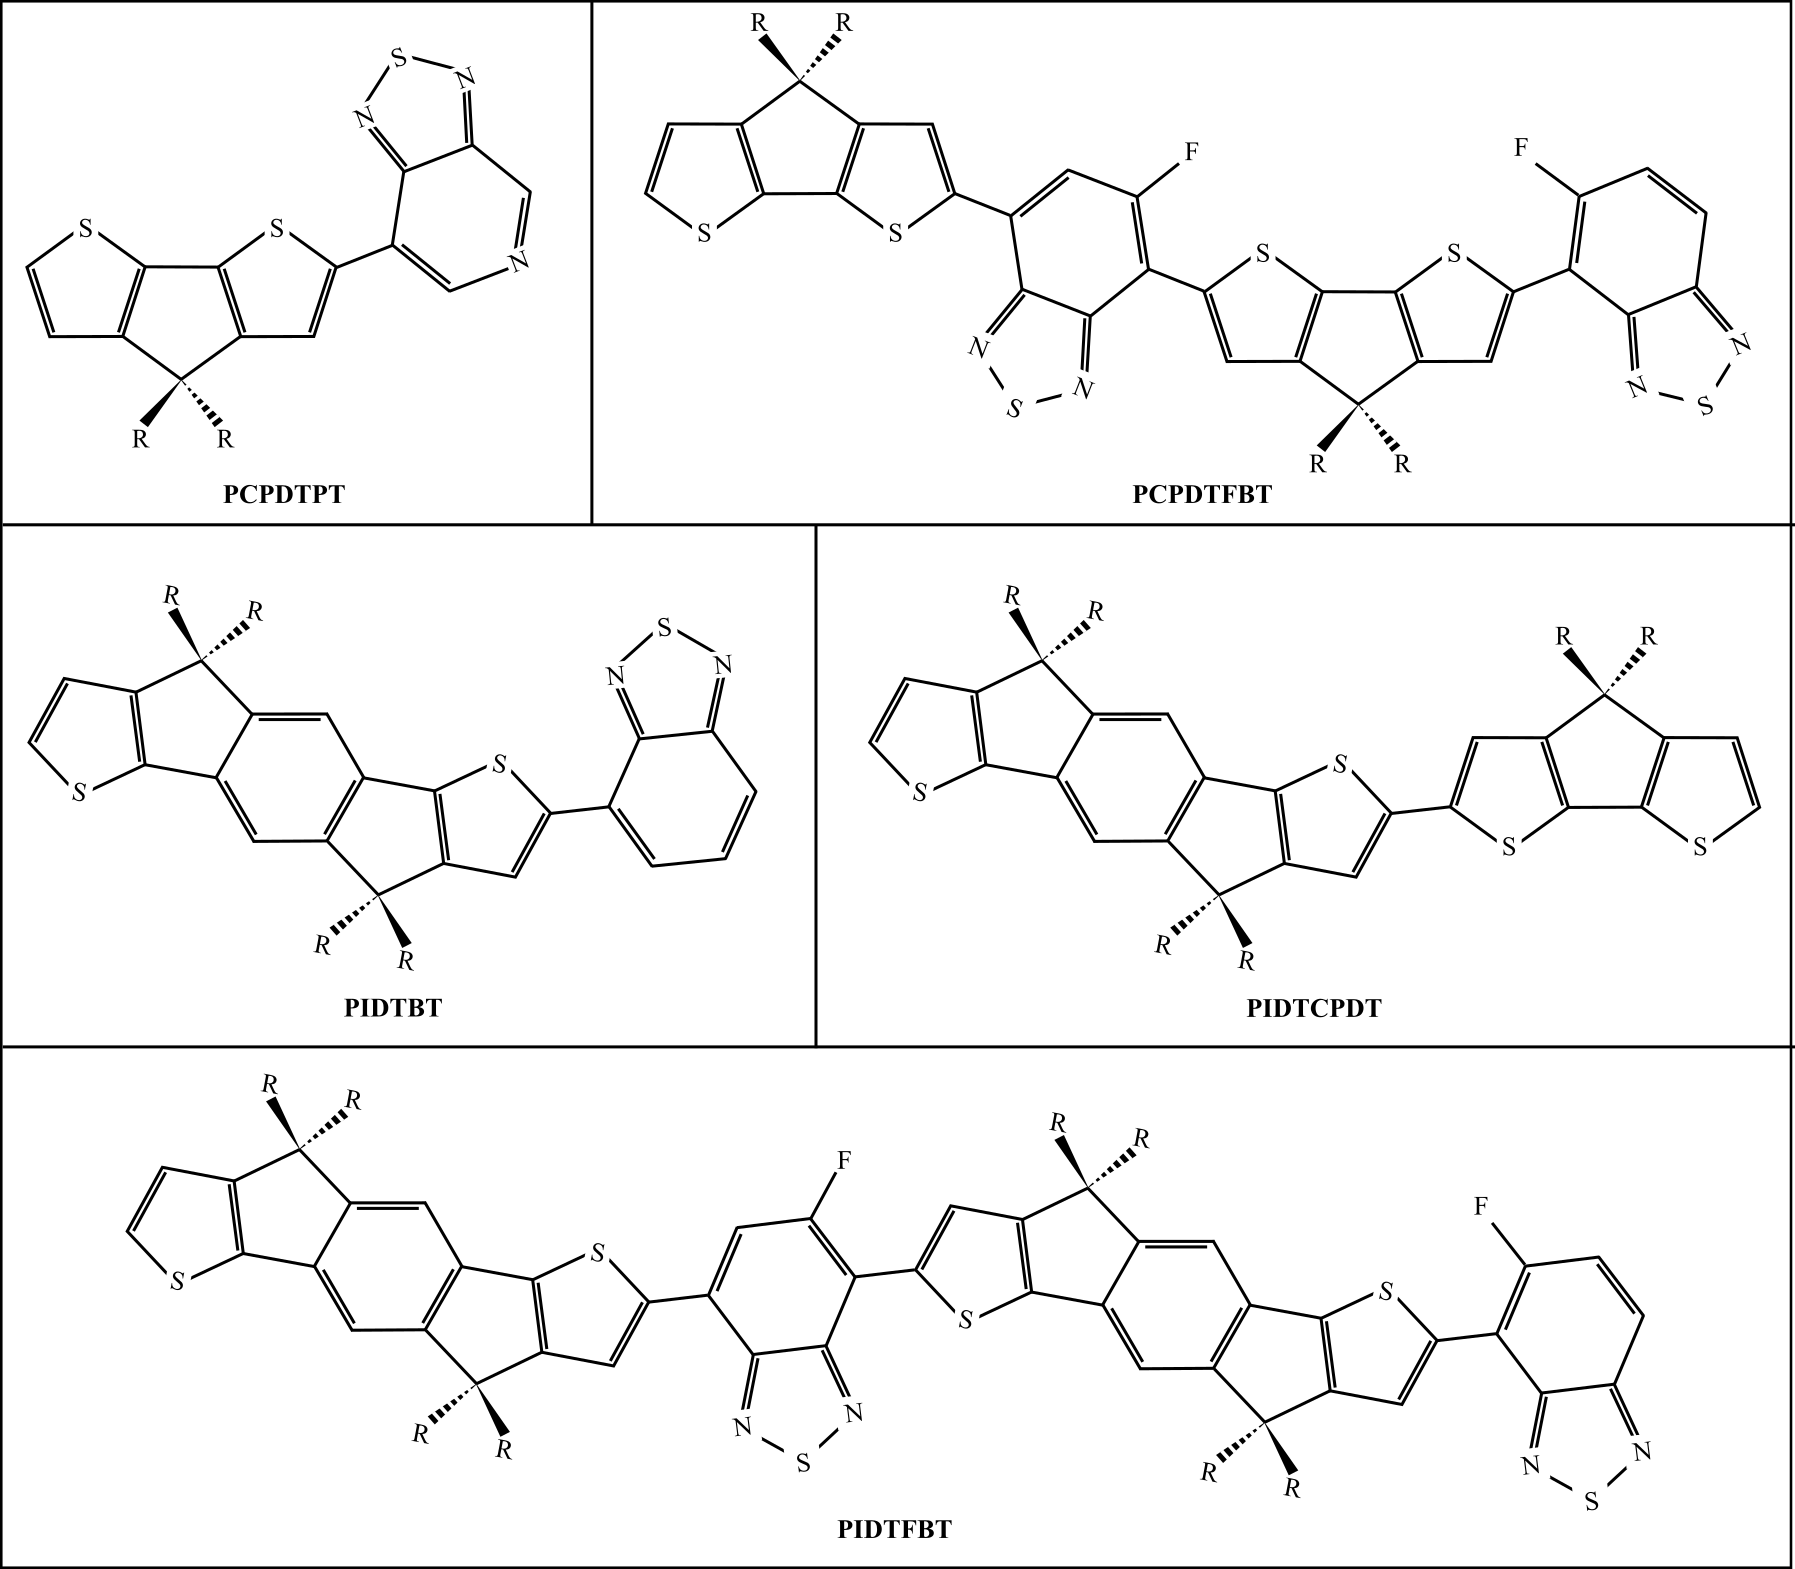
\includegraphics[width=0.9\linewidth]{src/figures/pers_l_figs/monomers.png}
    \caption{Molecular structures of the five repeating units used to build the polymers studied in this chapter. Each repeating includes a donor and acceptor region. }
    \label{fig:monomers}
\end{figure}
\newpage
\par The monomer fragments used to create the monomers in this study are cyclopentadithiophene (CPDT), pyridalthiadiazole (PT), benzothiadiazole (BT), fluorobenzothiadiazole (FBT), and indacenodithiophene (IDT). Each repeating was built to exhibit both donor and acceptor regions. \autoref{fig:monomers} depicts how the repeating units, or monomers were build from the monomer fragments listed above. The polymers with PIDTBT, PCPDTPT and PIDTCPDT backbones have an A-B-A-B polymerization pattern. PCPDTFBT and PIDTFBT polymers also consider the F functional group location, altering between a meta and an ortho position. The polymerization pattern for PIDTFBT and PCPDTFBT is A-B\textsubscript{m}-A-B\textsubscript{o}, where B\textsubscript{m} is meta-FBT and B\textsubscript{o} is ortho-FBT.  In this study, we investigate the effect of backbone chemistry as well as side chain complexity on the rigidity of the polymer, the side-chains are shown in \autoref{fig:rgroups}. Calculating the persistence length is not only a way to gain more of an understanding of polymer physics, but is also another means to validate the workflow developed in Chapter 4. 
\par We are using an implicit solvent model in this study, so we utilize temperature to mimic solvent effects, to justify this we must dive into polymer theory. We first need to define an ideal chain. An ideal chain is a model in polymer theory where monomer units along the polymer have no interactions. In a real chain, interactions would be observed between monomers as well as between the polymer and solvent. The theta temperature ($\Theta_{T}$) is the temperature at which a real polymer behaves as an ideal chain \citep{doi, rubin}. Similarly, the theta solvent ($\Theta_{S}$) is the solvent in which the polymer behaves as an ideal chain. Because we are modeling our solvent implicitly, we use the temperature to tune the ideality of our polymer chains, therefore mimicking how the solvent would effect chain behavior in experiment. We calculate the temperature at which we would expect the $l_p^{MD}$ and $l_p^{SANS}$ to match and compare this to the calculated $\Theta_{T}$ in order to draw conclusions on the solvent effects $C_6D_5Cl$ has on each polymer in the experimental data. 
\begin{figure}[h!]
    \centering
    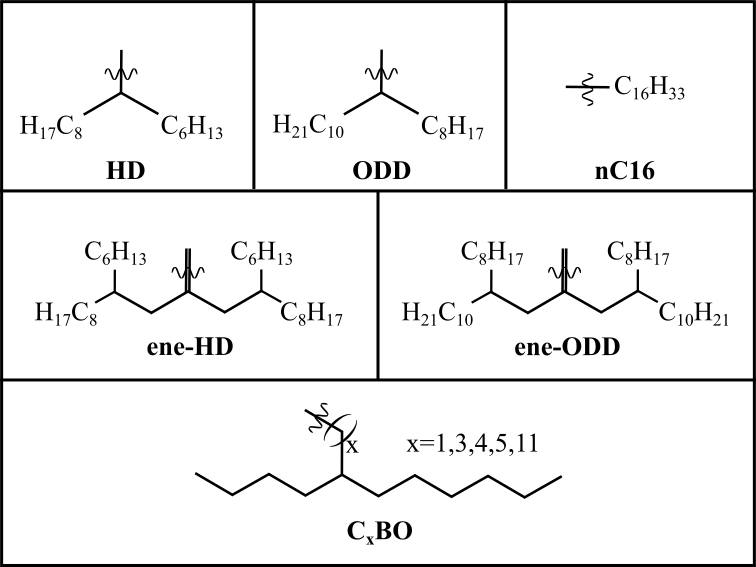
\includegraphics[width=0.8\linewidth]{src/figures/pers_l_figs/r_groups.png}
    \caption{Molecular structures of the six R-groups used as side chains in this study.}
    \label{fig:rgroups}
\end{figure}
\newpage

\section{Methods}
In this study, we conducted molecular dynamics simulations using \texttt{HOOMD-Blue} to investigate the persistence length of 13 various polymers. Simulations were performed on the Fry high performance computing cluster at Boise State using NVIDIA P100 and V100 GPUs. Each simulation was conducted in the canonical ensemble (NVT), in which the number of particles, volume, and temperature are all held constant throughout the simulation. Particle positions and velocities were updated using a two-step velocity-verlet integration of Newton’s laws of classical mechanics. The \texttt{FlowerMD} software package was utilized to construct our simulation object and initialize the simulations \citep{Albooyeh2023}. All simulations were initialized using the \texttt{Pack} functionality, in which the polymers are randomly placed in a cubic simulation box with periodic boundary conditions enforced. The simulation box size is calculated from the desired density, which is listed in \autoref{densities} for each polymer in \autoref{app:pers_len}. Thirteen conjugated polymers with similar backbone structures and varying side chain lengths were simulated in this study. An \texttt{espaloma} forcefield was generated for each polymer using the workflow outlined in Chapter 4. All simulations were run using an uncharged, united-atom model by removing the partial charges of each particle and adding the masses of the hydrogens into the neighboring, bonded atom. For each simulation we initialized a polymer of 250 monomer units in a large simulation space. Simulations were conducted at temperatures of
252, 503, 1006, 1258, 1510, 1761, 2013 K to capture how the persistence lengths evolve with temperature. The high temperatures were used to investigate how the persistence length might vary at high temperatures, but we focus on temperatures 252 K - 1006 K for analysis because temperatures above this are unrealistic for experimental settings. Simulations were run for $5 \times 10^7$ timesteps at a timestep size, dt = 0.001$\tau$. $\tau = \sqrt{M*L^2/E}$ , where M, L, and E are the reference mass, length, and energy of the simulation, respectively. From this information, the each timestep was 1.97 fs, resulting in a 98 ns simulation. 

\begin{wrapfigure}{l}{0.5\textwidth}
    \begin{center}
        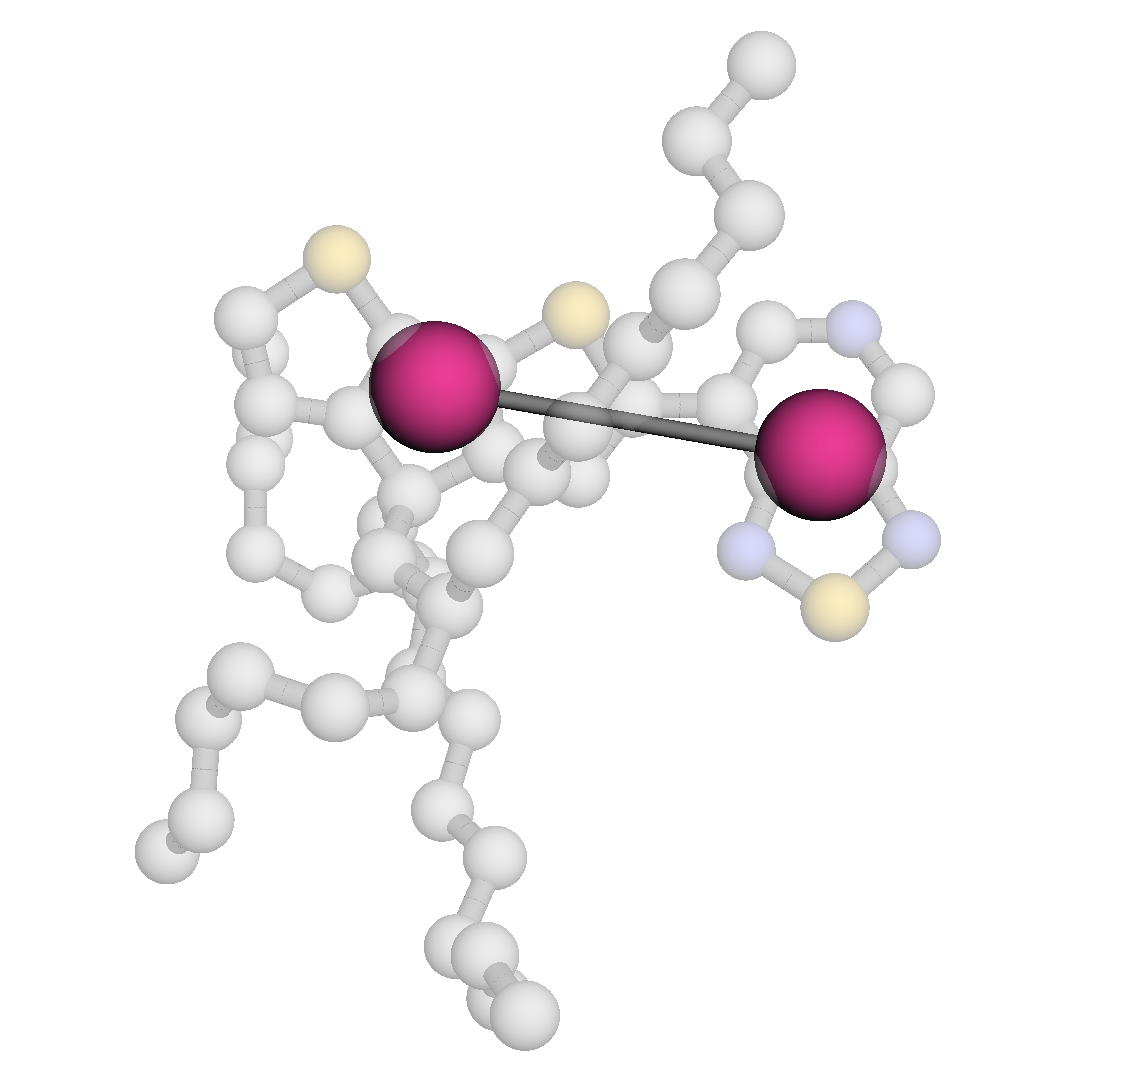
\includegraphics[width=0.48\textwidth]{src/figures/pers_l_figs/pcpdtpt_hd_cgmapping.png}
    \end{center}
  \caption{PCPDTPT-HD geometric centers used in calculating persistence length. The pink beads represent the monomer center of mass for the backbone molecules, CPDT on the left and PT on the right. The side chains were not included in the calculation of the center of mass.}
  \label{fig:CG_diagram}
\end{wrapfigure}

Once the simulations reached equilibrium and had at least 50 independent samples for each simulation the geometric center of masses were calculated using the GRiTS software \citep{grits}. This software takes an input of either the SMILES string for the portion of the molecule that you are replacing with a bead or the indices that should be replaced by a bead. In this study we used particle indices to manually determine where the beads should be placed rather than using SMILES string matching. In \autoref{fig:CG_diagram} we show an example of how a PCPDTPT-HD monomer's center of mass was calculated and where the sphere was placed. The beads are placed at the center of mass of the input indices provided by the user. The geometric centers were calculatedly adding a bead to each fully-rotatable unit to ensure that no sensitivity was lost in the persistence length calculation. 
The persistence length is determined to be the polymer length between the first monomer in the polymer chain and the first fully decorrelated monomer unit. A depiction of this is shown in \autoref{pers_length}. 
For this study, the persistence length was calculated by determining how each geometric center bead in the polymer correlates to the first bead at index 0. The correlation function ($C(n)$) is shown in \autoref{C_n1}. This equation explains how the angle correlation of the $n$\textsuperscript{th} bead is equal to the averaged dot products of the first bond vector ($\hat{a_{0}}$) and the $n$\textsuperscript{th} bond vector ($\hat{a_{0+n}}$). 
\begin{eqnarray}
  &&C(n) = \langle \cos{\theta_{0,0+n}} \rangle = \langle \hat{a_{0}} \cdot \hat{a_{0+n}} \rangle
  \label{C_n1}
\end{eqnarray}
The exponential relationship of the C(n) and n is shown in \autoref{C_n2}. The exponential coefficient of the autocorrelation function can be used to determine the persistence length, $l_p$ from the average bond lenght, $l_{b}$. 
\begin{eqnarray}
  &&C(n) \approx  \exp{\left(\frac{- n l_{b}}{l_{p}}\right)}  \approx \langle \hat{a_{0}} \cdot \hat{a_{0+n}} \rangle
  \label{C_n2}
\end{eqnarray}
Using these relationships, a python function was written to calculate $l_p$ of a polymer from the predicted morphology. In this function the autocorrelation of the bond vectors in the polymer backbone was calculated for 50 independent samples. The autocorrelation of each decorrelated snapshot was fit using the \texttt{curve\_fit function} in \texttt{SciPy's Optimize module} \citep{2020SciPy-NMeth}. Using the average bond length of the backbone bonds and the exponential coefficient gained from fitting the autocorrelation function to an exponential decay, the $l_p$ was calculated using the relationship in \autoref{C_n2}. The $l_p$'s for each snapshot were then averaged together and the standard deviations were calculated using \texttt{NumPy's Statistics module} \citep{numpy}. The full script for the persistence length function can be found at github.com/madilynpaul/persistence\_length as well as in \autoref{app:pers_len}. 
By plotting the root mean square end-to-end distance, $\sqrt{\langle R^2\rangle}$, versus the temperature of the simulation we were able to calculate the approximate theta temperature of each polymer. This was accomplished by determining the length at which the polymer will behave as an ideal chain, \autoref{e-e}. 
\begin{equation}
    \langle R^2 \rangle = N_{b}{l_b}^2
    \label{e-e}
\end{equation}
We then calculated the $\sqrt{\langle R^2\rangle}$ by taking the normalization of the end-to-end vector at each temperature and, using a linear regression, calculated the temperature at which the root mean square end-to-end distance was equivalent to $\sqrt{N_b}*{l_b}^2$, where $N_b$ is the number of bonds in the polymer and $l_b$ is the average bond length. The $\sqrt{\langle R^2\rangle}$ vs T plots can be found in \autoref{app:pers_len}. 
\section{Results and Discussion}
\begin{figure}[b]
    \centering
    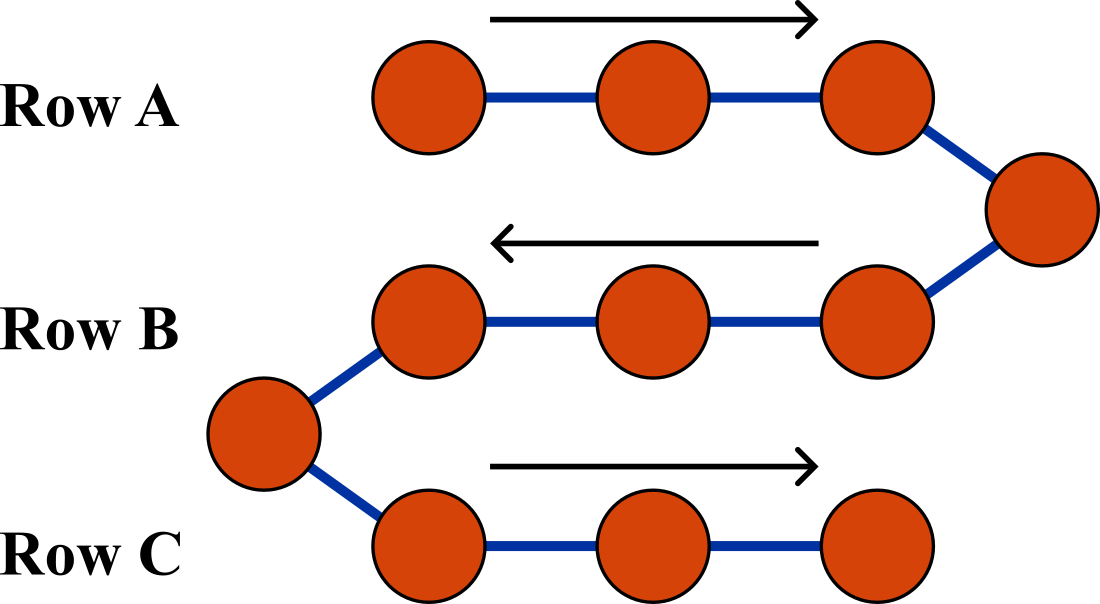
\includegraphics[width=0.5\linewidth]{src/figures/pers_l_figs/condensed_polymer.png}
    \caption{Diagram of a condensed polymer. Row A, B and C show the directions of the bond vectors. A snapshot of a condensed PCPDTPT-HD polymer can be found at \autoref{fig:real_cond_polymer}.}
    \label{fig:cond_polymer}
\end{figure}
We have successfully simulated 13 polymers with proven OPV properties. Each polymer consisted of 250 repeating units and was simulated in a large volume with no other molecules present. For most polymers we see an increase in persistence length as the temperature increases, until we reach a plateau in persistence length around 1000 K. This trend is expected, at lower temperatures we observe the polymers condensing and folding in on themselves (\autoref{fig:cond_polymer}), decreasing the persistence length. At temperatures above 1000 K the polymer has so much thermal energy it can easily overcome the steric hindrances leading to a more flexible polymer. 
\subsection{PCPDTPT Backbone}
The $l_p^{MD}$'s for polymers with a cyclopentadithiophene-co-pyridalthiadiazole (PCPDTPT) backbone (\autoref{fig:monomers}) are shown in \autoref{tab:lp_pcpdtpt}. The lower $l_p^{MD}$'s observed at lower temperatures is expected and can be explained using the diagram in \autoref{fig:cond_polymer}. When the polymer condenses on itself the $l_p$ decreases and non-bonded interactions between rows of the polymer (Rows A, B, and C ) become more prevalent. We observe good alignment between the $l_p^{MD}$'s calculated over this temperature range and the $l_p^{SANS}$'s calculated at room temperature. While we observe reasonable $l_p$ values, we do not observe the same trend in $l_p$ with increasing side chain size/complexity as the  $l_p^{SANS}$. The strong non-bonded interactions between side chains observed at low temperatures lead us to believe that having more than one polymer in the simulation is necessary for properly observing the side chain effects on backbone rigidity. 

\begin{table}[ht]
    \centering
    \begin{tabular}{c|c|c|c|c}
                        &  \multicolumn{4}{c}{\textbf{l\textsubscript{p}}}  \\
        \hline
        \textbf{Polymer}  & \textbf{252 K}& \textbf{503 K}& \textbf{1006 K}& \textbf{SANS}\\
        \hline
        PCPDTPT-ene-HD    &   $39.8 \pm 1.4$&	$48.4 \pm 1.2$&   $110.7 \pm 28$&    76.6   \\
        PCPDTPT-ene-ODD   &   $21.9 \pm 0.1$&	$38.5 \pm 1.1$&   $97.8 \pm 26$&    83.4   \\
        PCPDTPT-HD        &   $36.8 \pm 0.3$&	$55.3 \pm 9.3$&   $100.4 \pm 22$&    47.3   \\
        PCPDTPT-nC16      &   $40.2 \pm 0.7$&	$60.3 \pm 1.4$&   $96.0 \pm  22$&    61     \\
        PCPDTPT-ODD       &   $56.4 \pm 1.1$&	$63.6 \pm 2.6$&   $99.6 \pm 34$&    54.9   \\
    \end{tabular}
    \caption{Persistence lengths calculated from MD predicted morphologies ($l_p^{MD}$)  of polymers with a PCPDTPT backbone in comparison to persistence lengths calculated from SANS data ($l_p^{SANS}$). All $l_p$ presented in units of \AA.}
    \label{tab:lp_pcpdtpt}
\end{table}
By fitting the $l_p^{MD}$ with a linear regression we can predict what simulation temperature would give similar results to the SANS data. These linear regressions can be found in \autoref{app:pers_len}. Due to solvent effects we expect the $l_p^{SANS}$ values to align with different temperatures for each polymer. The simulation temperature at which we can predict similar $l_p^{MD}$ values to the $l_p^{SANS}$ values were predicted using a linear regression and can be found in \autoref{tab:sanT_pcpdtpt}. The backbone rigidity and temperature effects are not the only properties that can influence the persistence length. We can draw a connection between the solvent efficiency and the $l_p$. If the $T_{SANS}$ values are greater than the $\Theta_T$ we can conclude that the experimental solvent ($C_{6}D_{5}Cl$) is a good solvent for the given polymer. $C_{6}D_{5}Cl$ appears to be a good solvent for PCPDTPT-ene-HD, PCPDTPT-ene-ODD and PCPDTPT-n-C16, while it is a less than ideal solvent for PCPDTPT-HD and PCPDTPT-ODD. This comparison can be justified in the same manor that we explain the temperature effects on a polymer. If the polymer is solvated in a poor solvent it will condense into itself, and if it is a good solvent for the polymer we can expect that the polymer will extend into the solvent.
\begin{table}[ht]
    \centering
    \begin{tabular}{c|c|c|c}
    \textbf{Polymer}   &    \textbf{$T_{SANS}$} (K) &$\Theta_T$ (K) & $\textbf{$T_{SANS}$}/\Theta_T$\\
    \hline
    PCPDTPT-ene-HD     &    692 &502.5 & 1.38             \\
    PCPDTPT-ene-ODD    &    885 &456.2 & 1.94             \\
    PCPDTPT-HD         &    389 &507.0 & 0.767             \\
    PCPDTPT-nC16       &    526 &488.3 & 1.08             \\
    PCPDTPT-ODD        &    278 &450.5 & 0.616             \\
    \end{tabular}
    \caption{Predicted simulation temperature at which $l_p^{MD}$ would match $l_p^{SANS}$ for polymers with PCPDTPT backbone. $T_{SANS}$ calculated via linear regressions shown in \autoref{app:pers_len}. $T_{SANS}$ reported in units of K.}
    \label{tab:sanT_pcpdtpt}
\end{table}

\subsection{PCPDTFBT Backbone}
\par We observe similar trends in $l_p^{MD}$ with temperature as seen in the polymers with PCPDTPT backbones as we do with cyclopentadithiophene-co- fluorobenzothiadiazole (PCPDTFBT) backbone polymers. In PCPDTFBT-C1-BO, however, we observe a higher $l_p^{MD}$ at 503 K than at 1006 K. When calculating the $l_p$ by fitting the autocorrelation to an exponential function we don't take into account the bond vectors that may be aligned with the initial bond vector, but that shouldn't be contributing to the persistence length. This is a correction that would need to be accounted for in future calculations. The uncertainty at 1006 K is large enough to incorporate the $l_p^{MD}$ at 503 K, statistically stating that the the values are essentially equal. 
\begin{table}[ht]
    \centering
    \begin{tabular}{c|c|c|c|c}
                        &  \multicolumn{4}{c}{\textbf{l\textsubscript{p}}}  \\
        \hline
        \textbf{Polymer}  & \textbf{252 K}& \textbf{503 K}& \textbf{1006 K}& \textbf{SANS}\\
        \hline
        PCPDTFBT-C1-BO    &   $37.8 \pm 0.5$    &	$115.3 \pm 1.9$   &   $99.7 \pm 21$&    67	 \\
        PCPDTFBT-C3-BO    &   $47.5 \pm 0.4$    &	$57.6 \pm 2.8$    &   $98.9  \pm 22$&    78.4   \\
        PCPDTFBT-C4-BO    &   $46.3 \pm 1.1$    &	$65.8 \pm 3.1$    &   $105.1 \pm 20$&    86.4   \\
        PCPDTFBT-C5-BO    &   $35.4 \pm 0.3$    &	$68.7\pm 1.9$     &   $104.3 \pm 28$&    114	 \\
        PCPDTFBT-C11-BO   &   $34.6 \pm 0.2$    &	$55.9 \pm 2.6$    &   $104.0 \pm 26$&    291	 \\
    \end{tabular}
    \caption{Persistence lengths calculated from MD predicted morphologies ($l_p^{MD}$)  of polymers with a PCPDTFBT backbone in comparison to persistence lengths calculated from SANS data ($l_p^{SANS}$). All $l_p$ presented in units of \AA.}
    \label{tab:lp_pcpdtfbt}
\end{table}
\par The $l_p^{MD}$ values match well with the $l_p^{SANS}$ values for all polymers with the PCPDTFBT backbone besides that with the C11-BO side chain. The C11-BO side chain is much larger and bulkier than the other side chains, which could be contributing to the improper modeling. It could also be observed that PCPDTFBT-C11-BO may exhibit strong solvent interactions, in which solvent molecules would need to be present within the simulation to properly model the interactions. The fact that the polymers fold in on themselves and exhibit side chain interactions at low temperatures leads us to believe that a simulation with multiple polymers could lead to increased persistence lengths due to side chain interactions. 
\begin{table}[ht]
    \centering
    \begin{tabular}{c|c|c|c}
    \textbf{Polymer}   &    \textbf{$T_{SANS}$} (K) &$\Theta_T$ (K) & $\textbf{$T_{SANS}$}/\Theta_T$ \\
    \hline
    PCPDTFBT-C1-BO     &    326 &406.5    &      0.801   \\
    PCPDTFBT-C3-BO     &    736 &515.7    &      1.43   \\
    PCPDTFBT-C4-BO     &    767 &568.5    &      1.35    \\
    PCPDTFBT-C5-BO     &    1091 &491.9   &      2.22    \\
    PCPDTFBT-C11-BO    &    3034.7 &528.1 &      5.75       \\
    \end{tabular}
    \caption{Predicted simulation temperature at which $l_p^{MD}$ would match $l_p^{SANS}$ for polymers with PCPDTFBT backbone. $T_{SANS}$ calculated via linear regressions shown in \autoref{app:pers_len}. $T_{SANS}$ reported in units of K.}
    \label{tab:T_sans_pcpdtfbt}
\end{table}
\par The predicted simulation temperature at which the $l_p^{MD}$ and $l_p^{SANS}$ will match, $T_{SANS}$ can be found in \autoref{tab:T_sans_pcpdtfbt}, along with a comparison of the $\Theta_T$. The $T_{SANS}$ increases with increasing side chain size. $C_{6}D_{5}Cl$ appears to be a good solvent for all PCPDTFBT polymers besides PCPDTFBT-C1-BO, as $T_{SANS} < \Theta_T$. The values of $T_{SANS}$ are reasonable for all PCPDTFBT backbone polymers besides PCPDTFBT-C11-BO, with a value of 3034.7 K. In our MD model we observe a plateau in the persistence length at temperatures above 1200 K. The experimental values for persistence length of PCPDTFBT-C11-BO are larger than the greatest persistence lengths we observe. Investigations into our model as well as the model being used to fit the SANS data to calculate the persistence length are necessary in order to gain insight into the origin of these differences. 
\subsection{IDT Backbone}
The final DA co-polymers we investigated were ones with indacenodithiophene (IDT) as the donor molecule and three different acceptor molecules, CPDT, FBT, and BT. We successfully simulated these rather large co-polymers with little issues. The timesteps per second (TPS) for these simulations were significantly lower than the other polymer simulations due to the increased complexity and size of the polymer backbones. 
\begin{table}[ht]
    \centering
    \begin{tabular}{c|c|c|c|c}
                        &  \multicolumn{4}{c}{\textbf{l\textsubscript{p}}}  \\
        \hline
        \textbf{Polymer}  & \textbf{252 K}& \textbf{503 K}& \textbf{1006 K}& \textbf{SANS}\\
        \hline
        PIDTBT-nC16       &   $65.4\pm 0.2$     &	$57.8 \pm 1.6$&   $200.6 \pm 26$&    1310   \\
        PIDTCPDT-C11-BO   &   $36.0 \pm 0.2$    &	$76.4 \pm 8.7$&   $182.2 \pm 49$&    236	 \\
        PIDTFBT-C11-BO    &   $79.4 \pm 3.9$    &	$90.6 \pm 23$&  $178.4 \pm 32.7$    &    254	 \\
    \end{tabular}
    \caption{Persistence lengths calculated from MD predicted morphologies ($l_p^{MD}$)  of polymers with a IDT backbone in comparison to persistence lengths calculated from SANS data ($l_p^{SANS}$). All $l_p$ presented in units of \AA.}
    \label{tab:lp_pidt}
\end{table}
We have predicted reasonable values for $l_p^{MD}$, we observe an increase in $l_p^{MD}$ with the increase in temperature, with only one outlier of PIDTBT-nC16 at 503 K, \autoref{tab:lp_pidt}. We also observe good overlap between the $l_p^{MD}$ and $l_p^{SANS}$ for the PIDTFBT-C11-BO and PIDTCPDT-C11-BO polymers. Molecular dynamics predicts a significantly lower $l_p^{MD}$ for PIDTBT-nC16 than the presented $l_p^{SANS}$. However, the $l_p^{SANS}$ for all three of these polymers is reported as longer than the contour length ($L_c$) of the polymer in experiment. This makes the direct comparison of  $l_p^{MD}$ and $l_p^{SANS}$ ineffective. Both the experimental and DFT values presented for these three co-polymers came with some caveats, leading us to believe that the method of analysis used in calculating $l_p^{DFT}$ and $l_p^{SANS}$ breaks down with larger, more complex polymers requiring additional steps to predict the $l_p^{DFT}$. For all three IDT polymers the $l_p^{SANS}$ reported is longer than the contour length of the polymer, due to the $l_p^{SANS}$>$L_c$  fitting the $l_p^{SANS}$ into the linear regression of $l_p^{MD}$ results in very high, inaccurate $T_{sans}$ values. Again, due to the plateau observed in $l_p^{MD}$ at temperatures above 1200 K, we cannot confidently say that simulating these polymers at the $T_{SANS}$ temperature will result in $l_p^{MD} \approx l_p^{SANS}$. Further investigation into both theoretical and experiential results are necessary to draw conclusions. 
\begin{table}[ht]
    \centering
    \begin{tabular}{c|c|c|c}
    \textbf{Polymer}   &    \textbf{$T_{sans}$} (K) &$\Theta_T$ (K) & $\textbf{$T_{SANS}$}/\Theta_T$\\
    \hline
    PIDTBT-nC16        &    6785 &411.7 & 16.5             \\
    PIDTCPDT-C11-BO    &    1290 &511.1 & 2.52             \\
    PIDTFBT-C11-BO     &    1591 &405.0 & 3.93             \\
    \end{tabular}
    \caption{Predicted simulation temperature at which $l_p^{MD}$ would match $l_p^{SANS}$ for polymers with IDT backbone. $T_{SANS}$ calculated via linear regressions shown in \autoref{app:pers_len}. $T_{SANS}$ reported in units of K.}
    \label{tab:T_sans_pidt}
\end{table}
\subsection{MD vs DFT}
\begin{table}[ht]
    \centering
    \begin{tabular}{l|l|ll}
         \textbf{Polymer} & \textbf{$l_p^{DFT}$}& \textbf{$l_p^{MD}$} &\textbf{$l_p^{SANS}$}\\
         \hline
         PCPDTFBT-C1-BO     & 71.1              &   $99.7  \pm 21$ &67\\
         PCPDTFBT-C3-BO     & 71.1              &   $98.9  \pm 22$ &78.4   \\
         PCPDTFBT-C4-BO     & 71.1              &   $105.1 \pm 20$ &86.4   \\
         PCPDTFBT-C5-BO     & 71.1              &   $104.3 \pm 28$ &114\\
         PCPDTFBT-C11-BO    & 71.1              &   $104.0 \pm 26$ &291\\
         PCPDTPT-ene-HD     & 48.0              &   $110.7 \pm 28$ &76.6   \\
         PCPDTPT-ene-ODD    & 48.0              &   $97.8 \pm 26$ &83.4   \\
         PCPDTPT-HD         & 44.9              &   $100.4 \pm 22$ &47.3   \\
         PCPDTPT-nC16       & 44.9              &   $96.0 \pm  22$ &61     \\
         PCPDTPT-ODD        & 44.9              &   $99.6 \pm 34$ &54.9   \\
         PIDTBT-nC16        & ($>$1 \(\mu\)m)   &   $200.6 \pm 26$ &1310   \\
         PIDTCPDT-C11-BO    & 224               &   $182.2 \pm 49$ &236\\
         PIDTFBT-C11-BO     & ($>$1 \(\mu\)m)   &   $178.4 \pm 33$ &254\\
    \end{tabular}
    \caption{A comparison of $l_p^{DFT}$ reported by Danielsen, et al.~ at Ref \citep{danielsen_chain_2022} to $l_p^{MD}$ calculated at a temperature of 1006 K.}
    \label{dft_lps}
\end{table}
The results reported by Danielsen, et al.~ for $l_p^{DFT}$ are presented in \autoref{dft_lps} as well at the $l_p^{MD}$ and the $l_p^{SANS}$ \citep{danielsen_chain_2022}. Dihedral potentials were calculated using optimized scans of the central dihedral angle ($\phi$) of each monomer unit \citep{milner}. To minimize computational cost monomer units were utilized rather than polymers and side chains were replaced by methyl groups. A numerical average of backbone conformations was estimated from a set of dihedral angles, from this the $l_p^{DFT}$ was approximated. In the DFT approach accuracy is lost in modeling all side chains as methyl groups and only modeling one monomer unit. The DFT approach also does not model temperature or solvents, whereas MD simulations are able to model long polymers, complex side chains as well as temperature and can be easily modified to model explicit solvents. 

\section{Conclusions}
The molecular dynamics approach presented here has a significantly lower computational cost, allowing for the simulation of long oligomers with full side chains. Both these factors add to our confidence in the accuracy of the persistence length calculations. We observe that molecular simulations can predict side-chain influences on persistence length. The calculated $l_p^{MD}$ show good agreement to the $l_p^{SANS}$ for the majority of the polymers in this study in terms of magnitudes and trends. From this information we can conclude that the MD workflow presented in Chapter 4 is accurately predicting bulk morphologies of DA-polymers. From this work we conclude that $l_p$ is a relatively simple measure of the thermodynamic stability of a polymer as well as a prediction of the bulk morphology and we present a MD workflow that accurately predicts and calculates the $l_p$ of DA co-polymers. 
%------------------------------------------------------------------------------
\chapter{Conclusions}
\label{chap:Conclusions}

Over the course of this dissertation we have tied together two very different, but theoretically similar projects. Beginning with attempting to model the polymorphic phase transition of barbituric acid dihydrate, we discovered that what was reported to be a very subtle phase transition at 217 K was actually the presence of crystalline disorder. We aimed to model this phase transition via density functional theory (DFT) due to the present of hydrate molecules in the crystal structure, but when two equivalent energy well were observed in the potential energy scan of the structure at temperatures above 217 K it became clear that this phase transition might not exist. This paired with the widening of the peaks in the terahertz spectra, lead us to conclude that there was twinning within the crystalline structure. Further investigation into this revealed that above 217 K the molecules had enough energy to oscillate between the two energetically favorable configurations. When this structure was analyzed using x-ray crystallography the oscillating molecule's positions were averaged out into a perfectly planar configuration, leading the investigators to report that the molecules were confined to a \textit{Pnma} space group. Upon finding this crystal disorder we became skeptical of the planar configuration reported for violuric acid monohydrate because of the similarities in structure between the two compounds. When investigating VAMH a double-welled potential and imaginary mode lead us to prematurely conclude that VAMH had a space group of \textit{P}2\textsubscript{1} rather than \textit{Cmc}2\textsubscript{1}. When evaluating the terahertz spectra of VAMH generated in the \textit{P}2\textsubscript{1} space group to the experimental there was not good peak alignment. This led us to increase the size of the unit cell and remove all symmetry operations, allowing the molecules to freely optimize. The molecules were then perceived to belong to the orthorhombic \textit{Pca}2\textsubscript{1} space group. In this space group the double-welled potential disappeared and the experimental spectra aligned well with the theoretical spectra. 
The second half of this dissertation focused on developing tools for structure determination via molecular dynamics. With a focus on organic macromolecules and polymers we developed a workflow that implemented Espaloma generated forcefields into the molecular dynamics framework. It was necessary to validate the accuracy of the Espaloma forcefields for conjugated, organic molecule before using the workflow to predict morphologies of these kinds of materials. To validate the workflow we predicted the morphologies of two widely studied organic molecules, perylene and poly-3-hexylthiophene (P3HT). We found that Espaloma produces similar forcefield parameters to the generalized amber forcefield (GAFF). The predicted morphologies of both materials with the espaloma forcefield showed great overlap with those predicted using the OPLS-UA forcefield. Once the workflow was validated for this use we utilized it to predict the morphologies of 13 conjugated donor-acceptor co-polymers over a range of temperatures. A function was written to calculate the persistence length from the predicted morphologies of the 13 polymers. This function was validated against persistence lengths calculated via DFT and small angle neutron scattering patterns. 
%------------------------------------------------------------------------------
% bibliography:
% \cleardoublepage
\addcontentsline{toc}{chapter}{References} 
\bibliography{src/bibliography}
\bibliographystyle{unsrt}
%------------------------------------------------------------------------------
% \cleardoublepage
\addcontentsline{toc}{chapter}{Appendices}
\appendix
\chapter{Espaloma Function Code}
\label{app:esp_function_code}

\begin{figure}
    \centering
    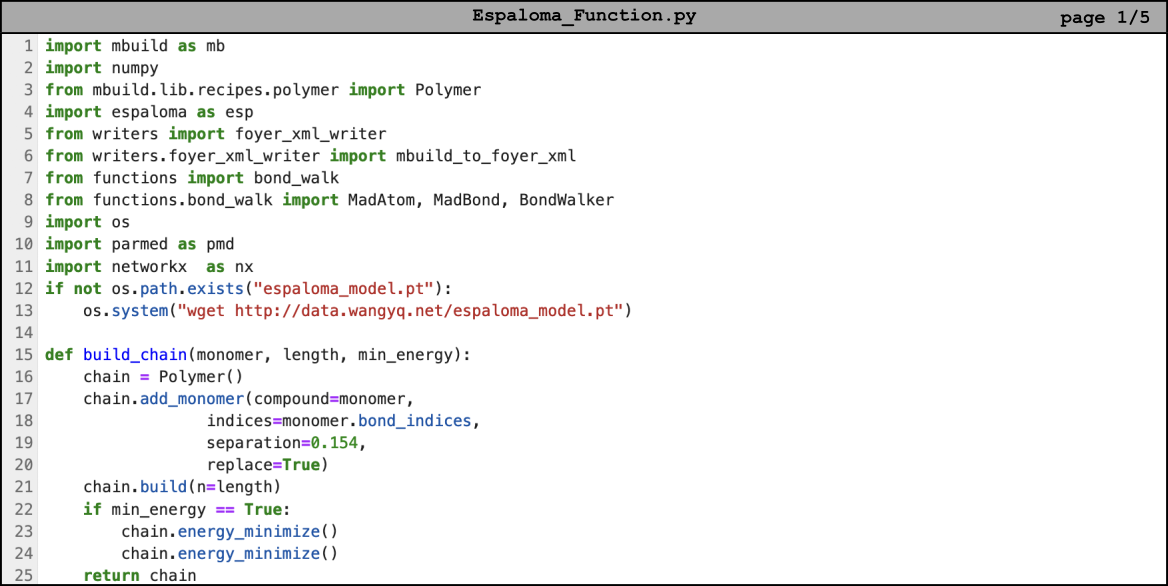
\includegraphics[width=1\linewidth]{src/figures/FF_figs/esp1.png}
    \label{fig:esp1}
\end{figure}

\begin{figure}
    \centering
    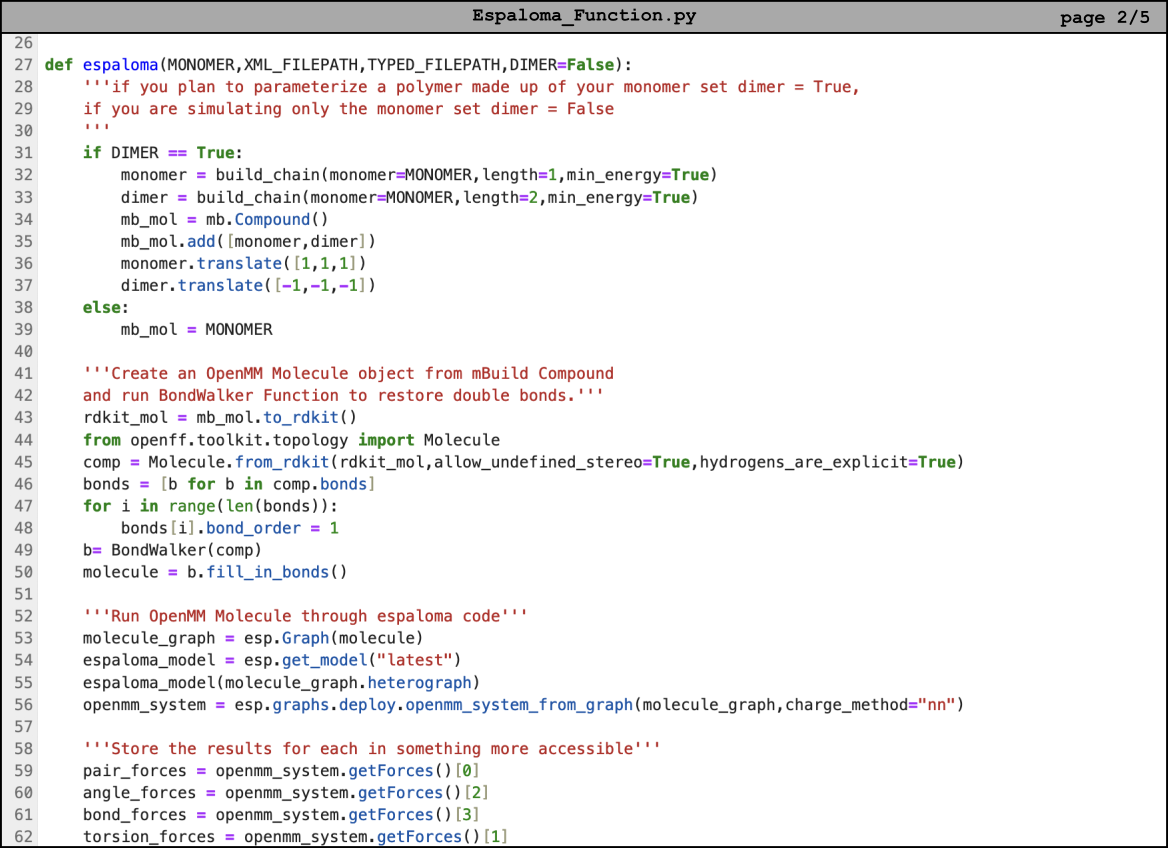
\includegraphics[width=1\linewidth]{src/figures/FF_figs/esp2.png}
    \label{fig:esp2}
\end{figure}

\begin{figure}
    \centering
    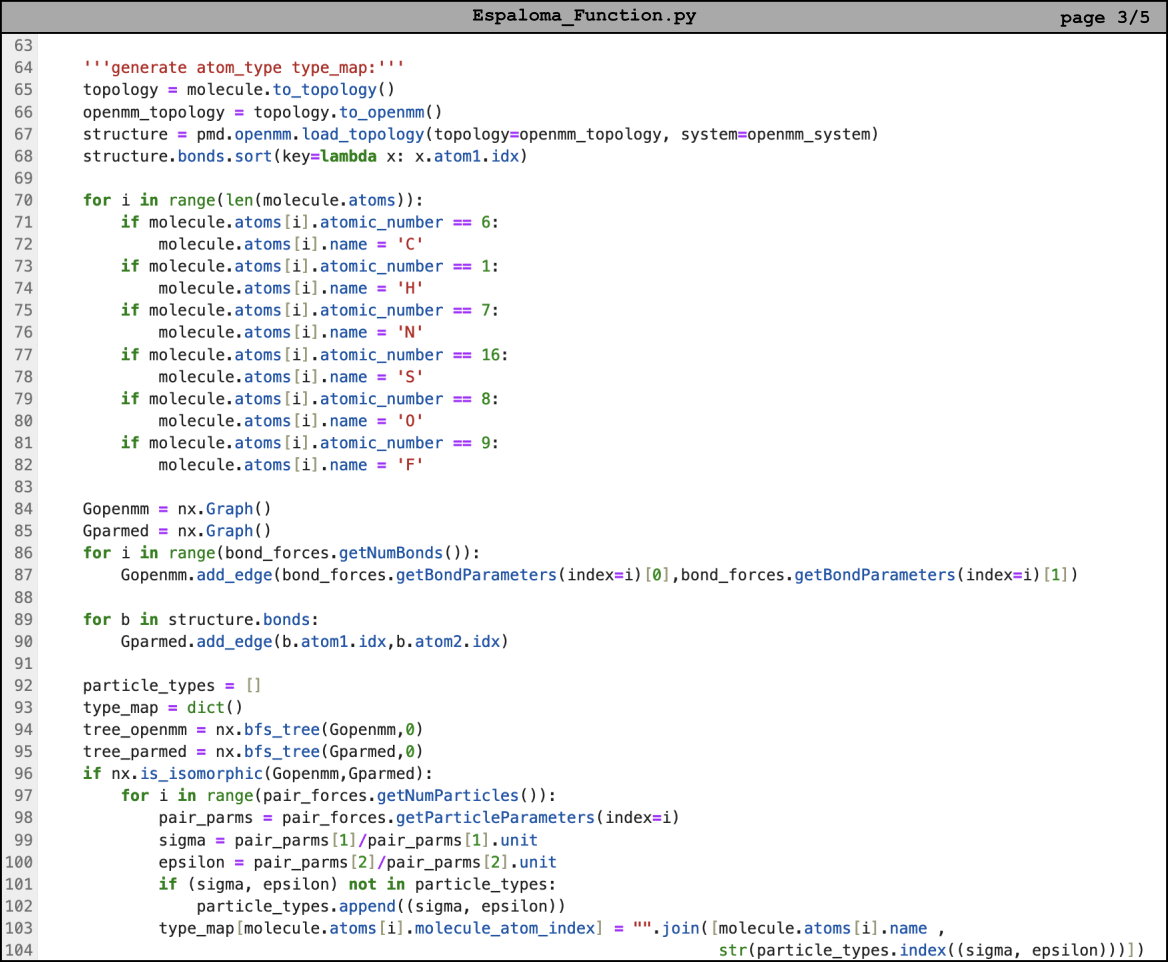
\includegraphics[width=1\linewidth]{src/figures/FF_figs/esp3.png}
    \label{fig:esp3}
\end{figure}

\begin{figure}
    \centering
    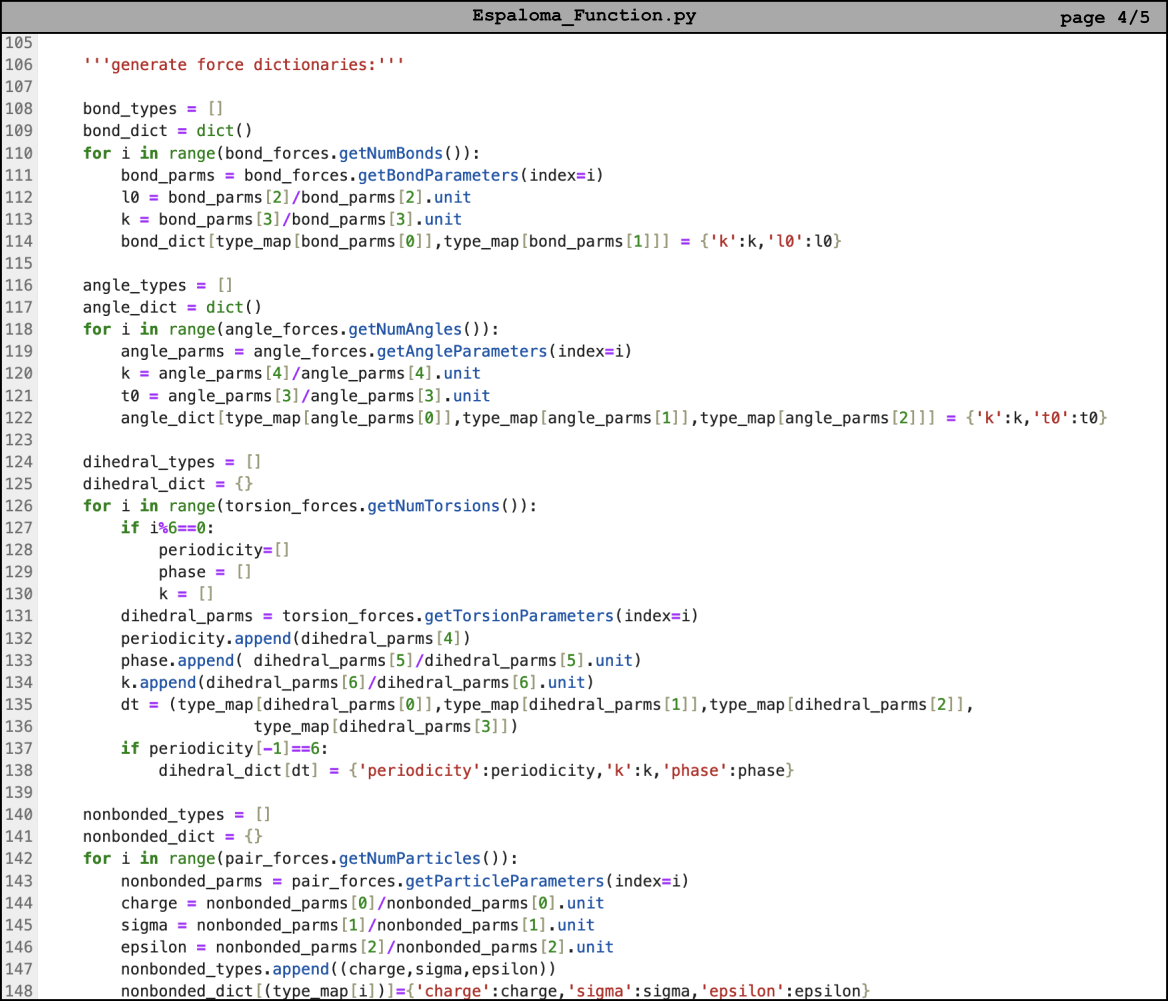
\includegraphics[width=1\linewidth]{src/figures/FF_figs/esp4.png}
    \label{fig:esp4}
\end{figure}

\begin{figure}
    \centering
    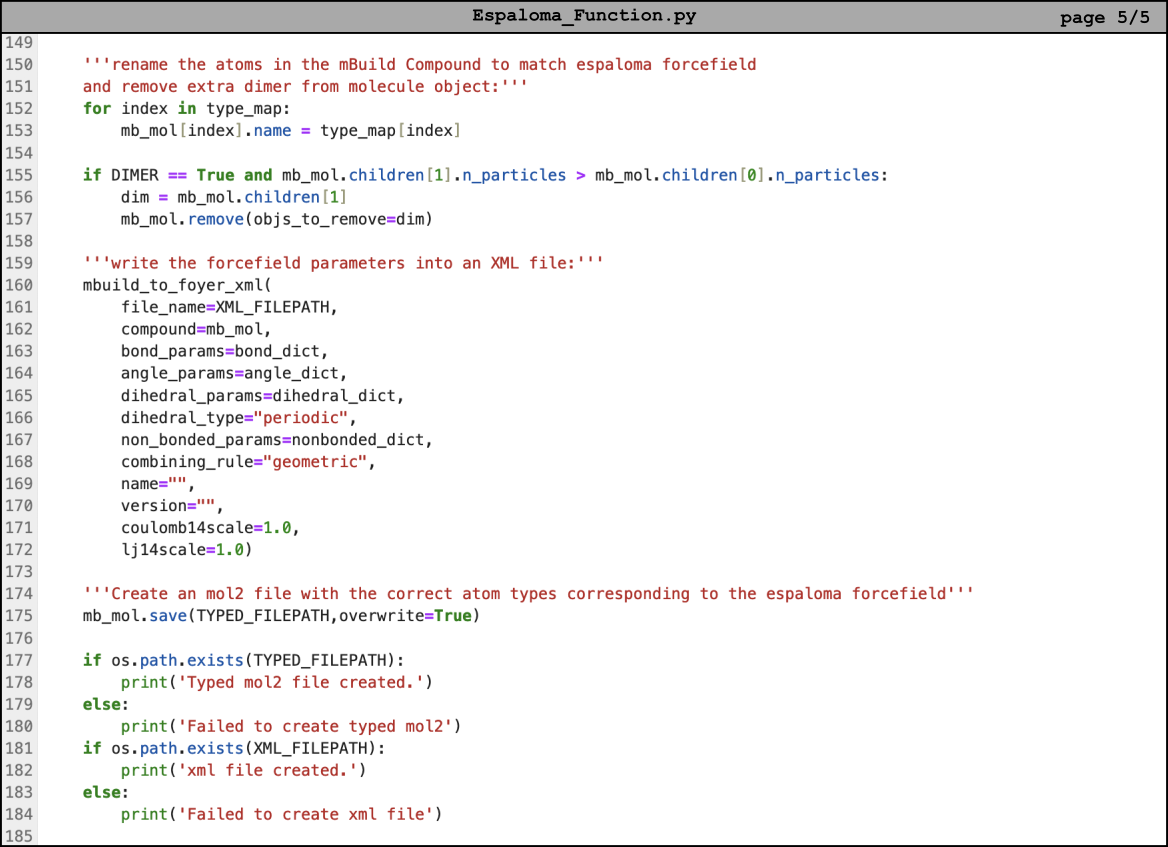
\includegraphics[width=1\linewidth]{src/figures/FF_figs/esp5.png}
    \label{fig:esp5}
\end{figure}

\chapter{Bond Walker Example Code}
\label{app:bond_walker_code}

\begin{figure}
    \centering
    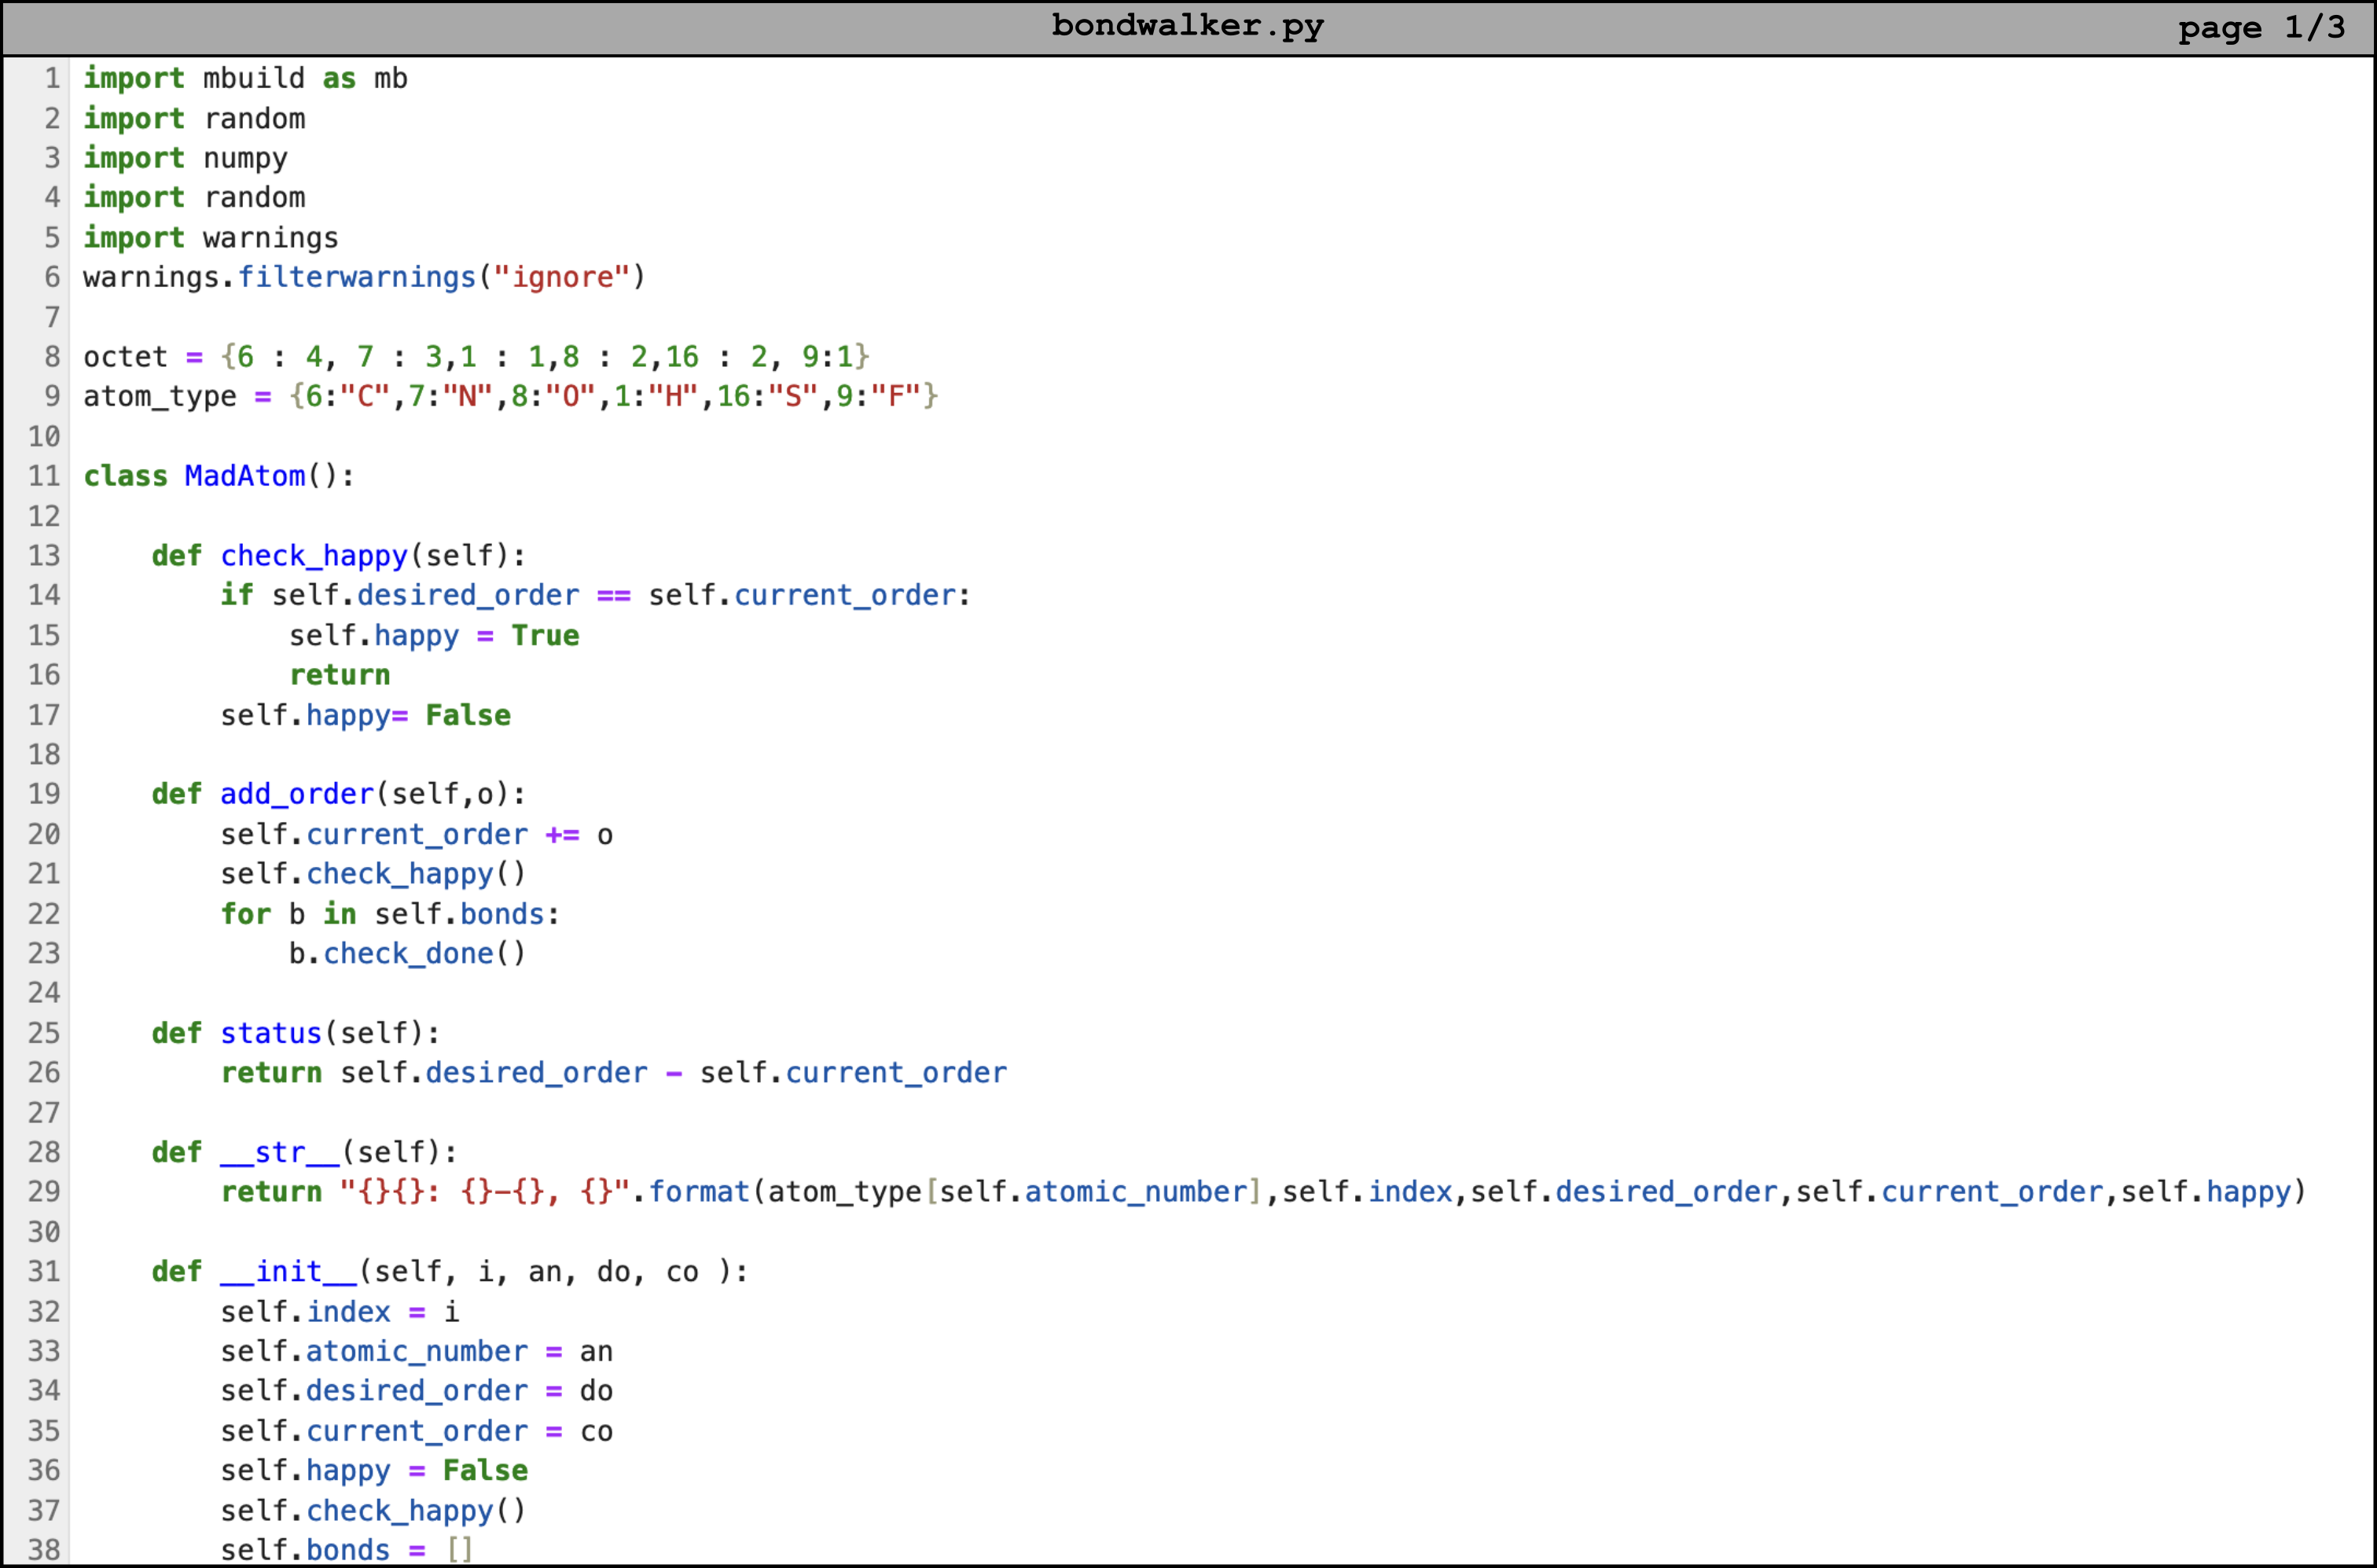
\includegraphics[width=1\linewidth]{src/figures/FF_figs/bw1.png}
    \label{fig:bw1}
\end{figure}


\begin{figure}
    \centering
    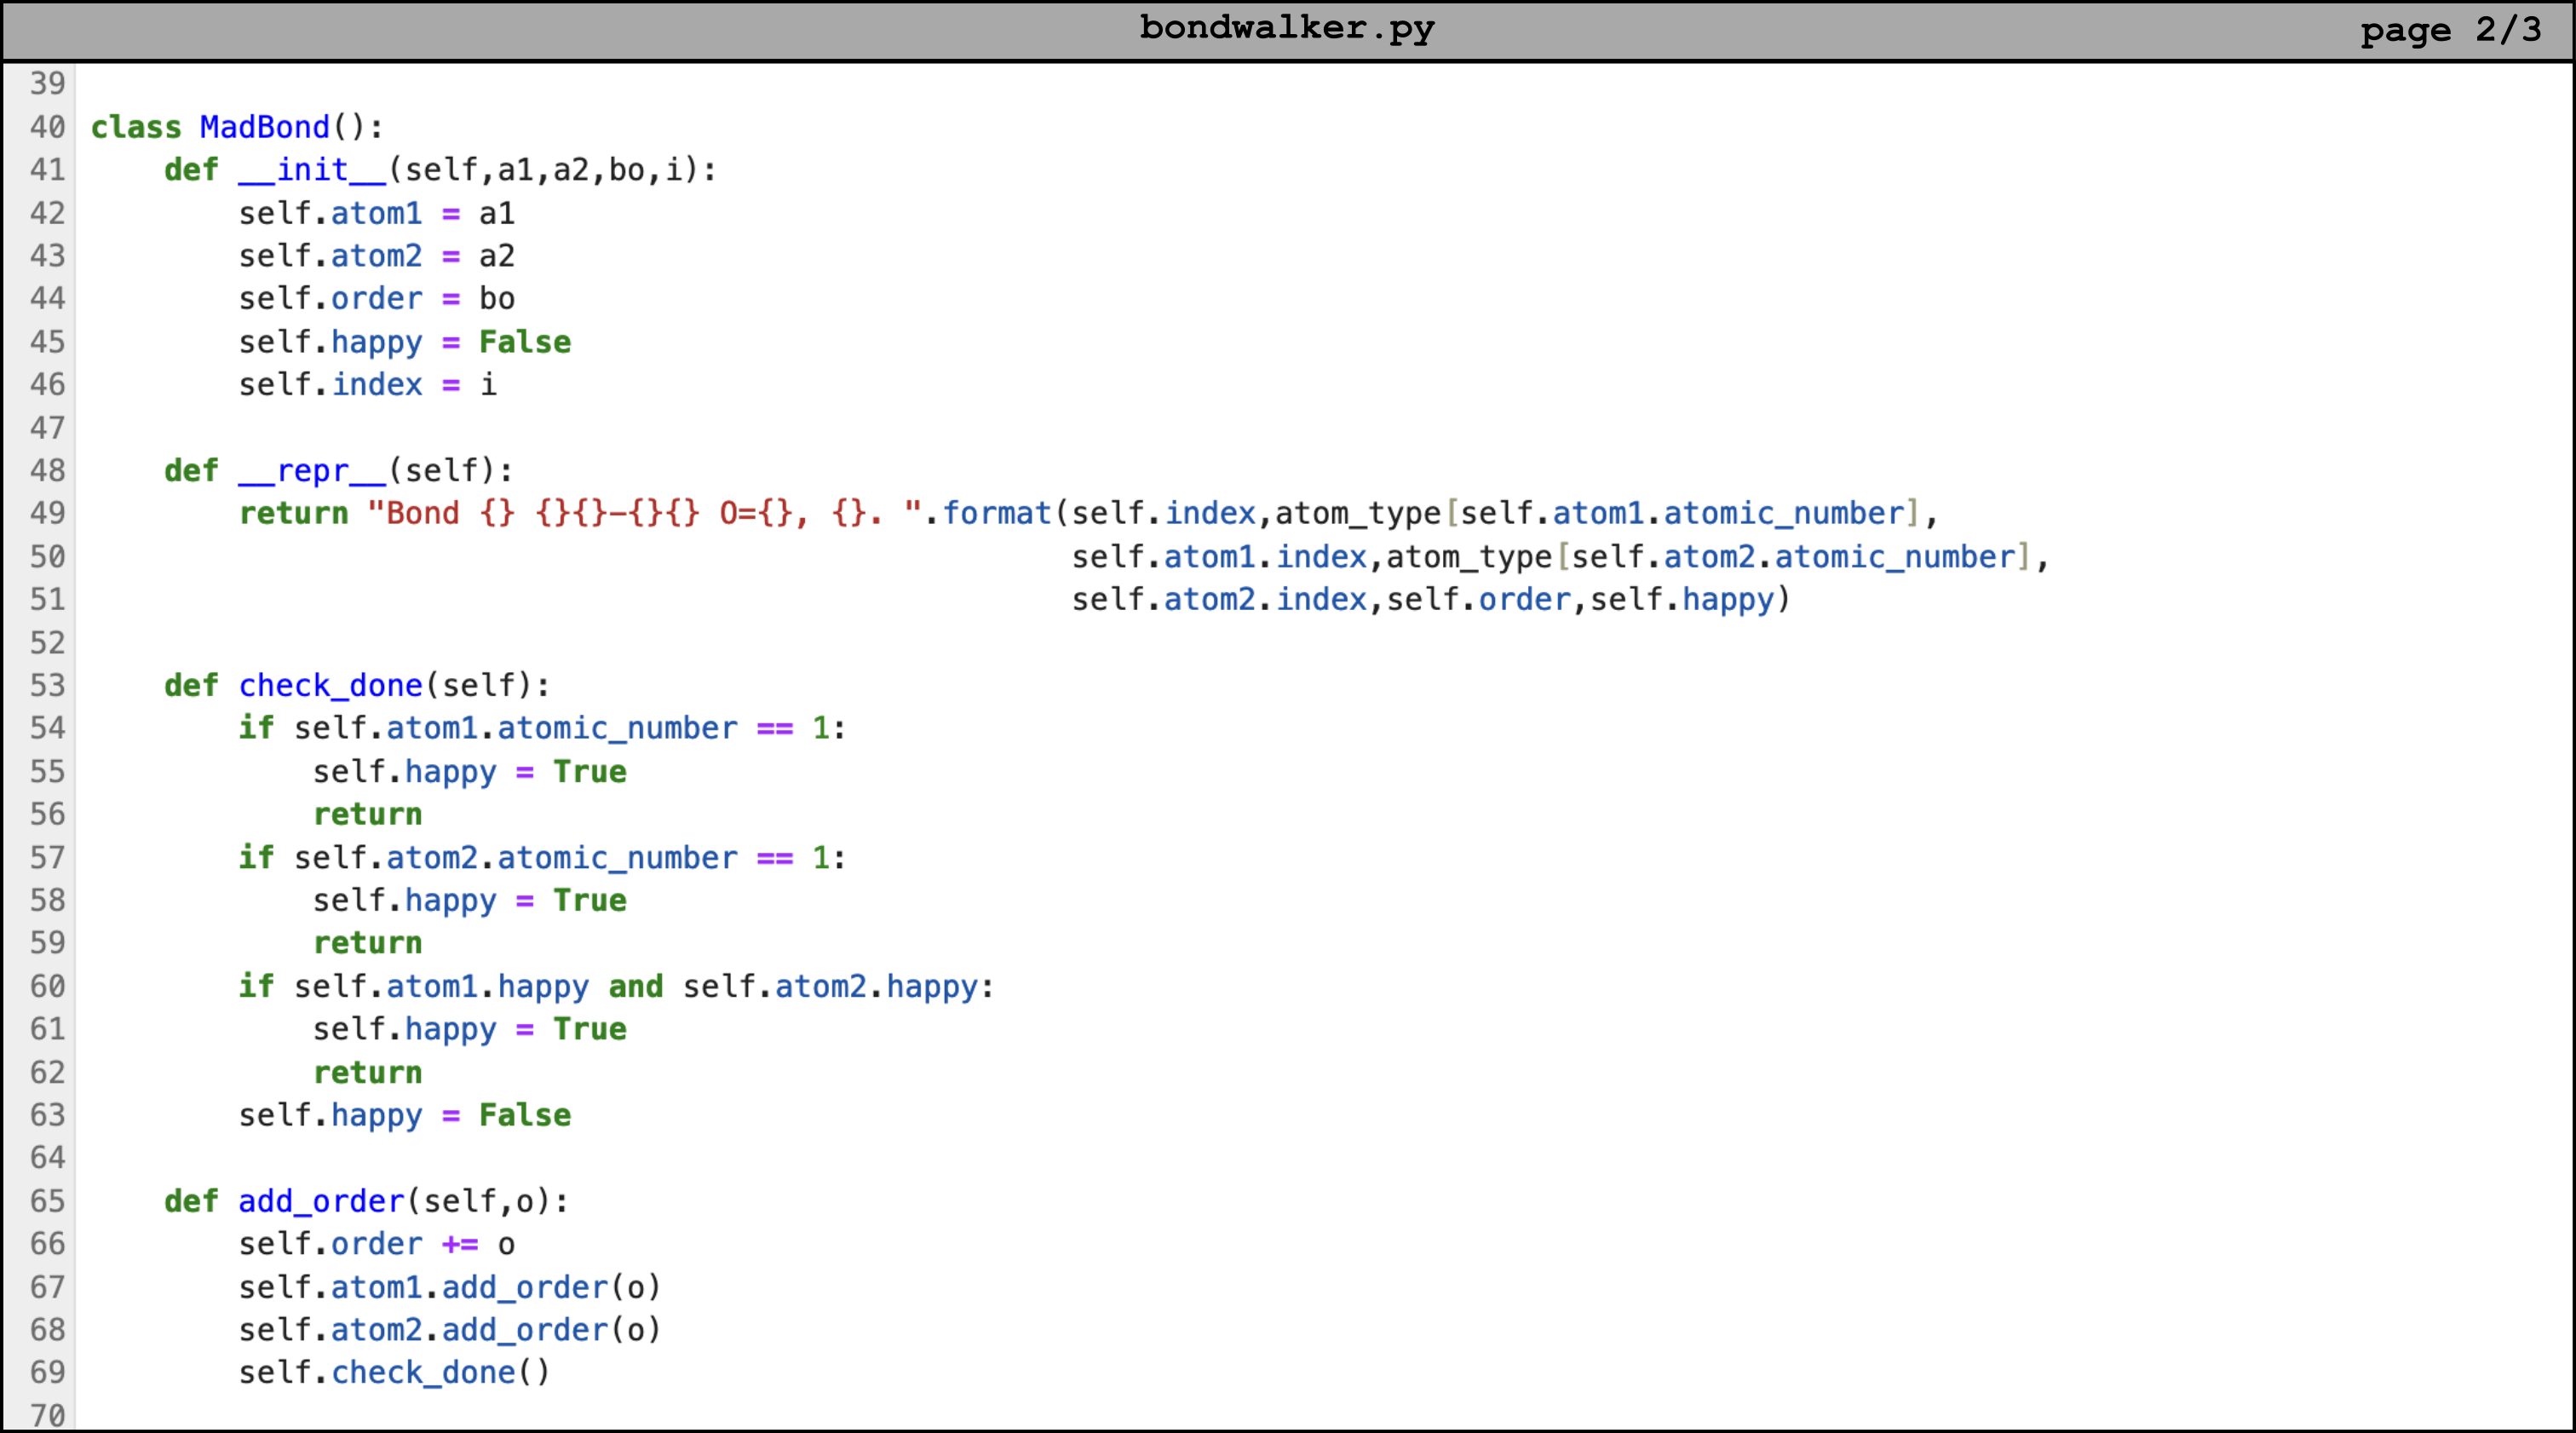
\includegraphics[width=1\linewidth]{src/figures/FF_figs/bw2.png}
    \label{fig:bw2}
\end{figure}


\begin{figure}
    \centering
    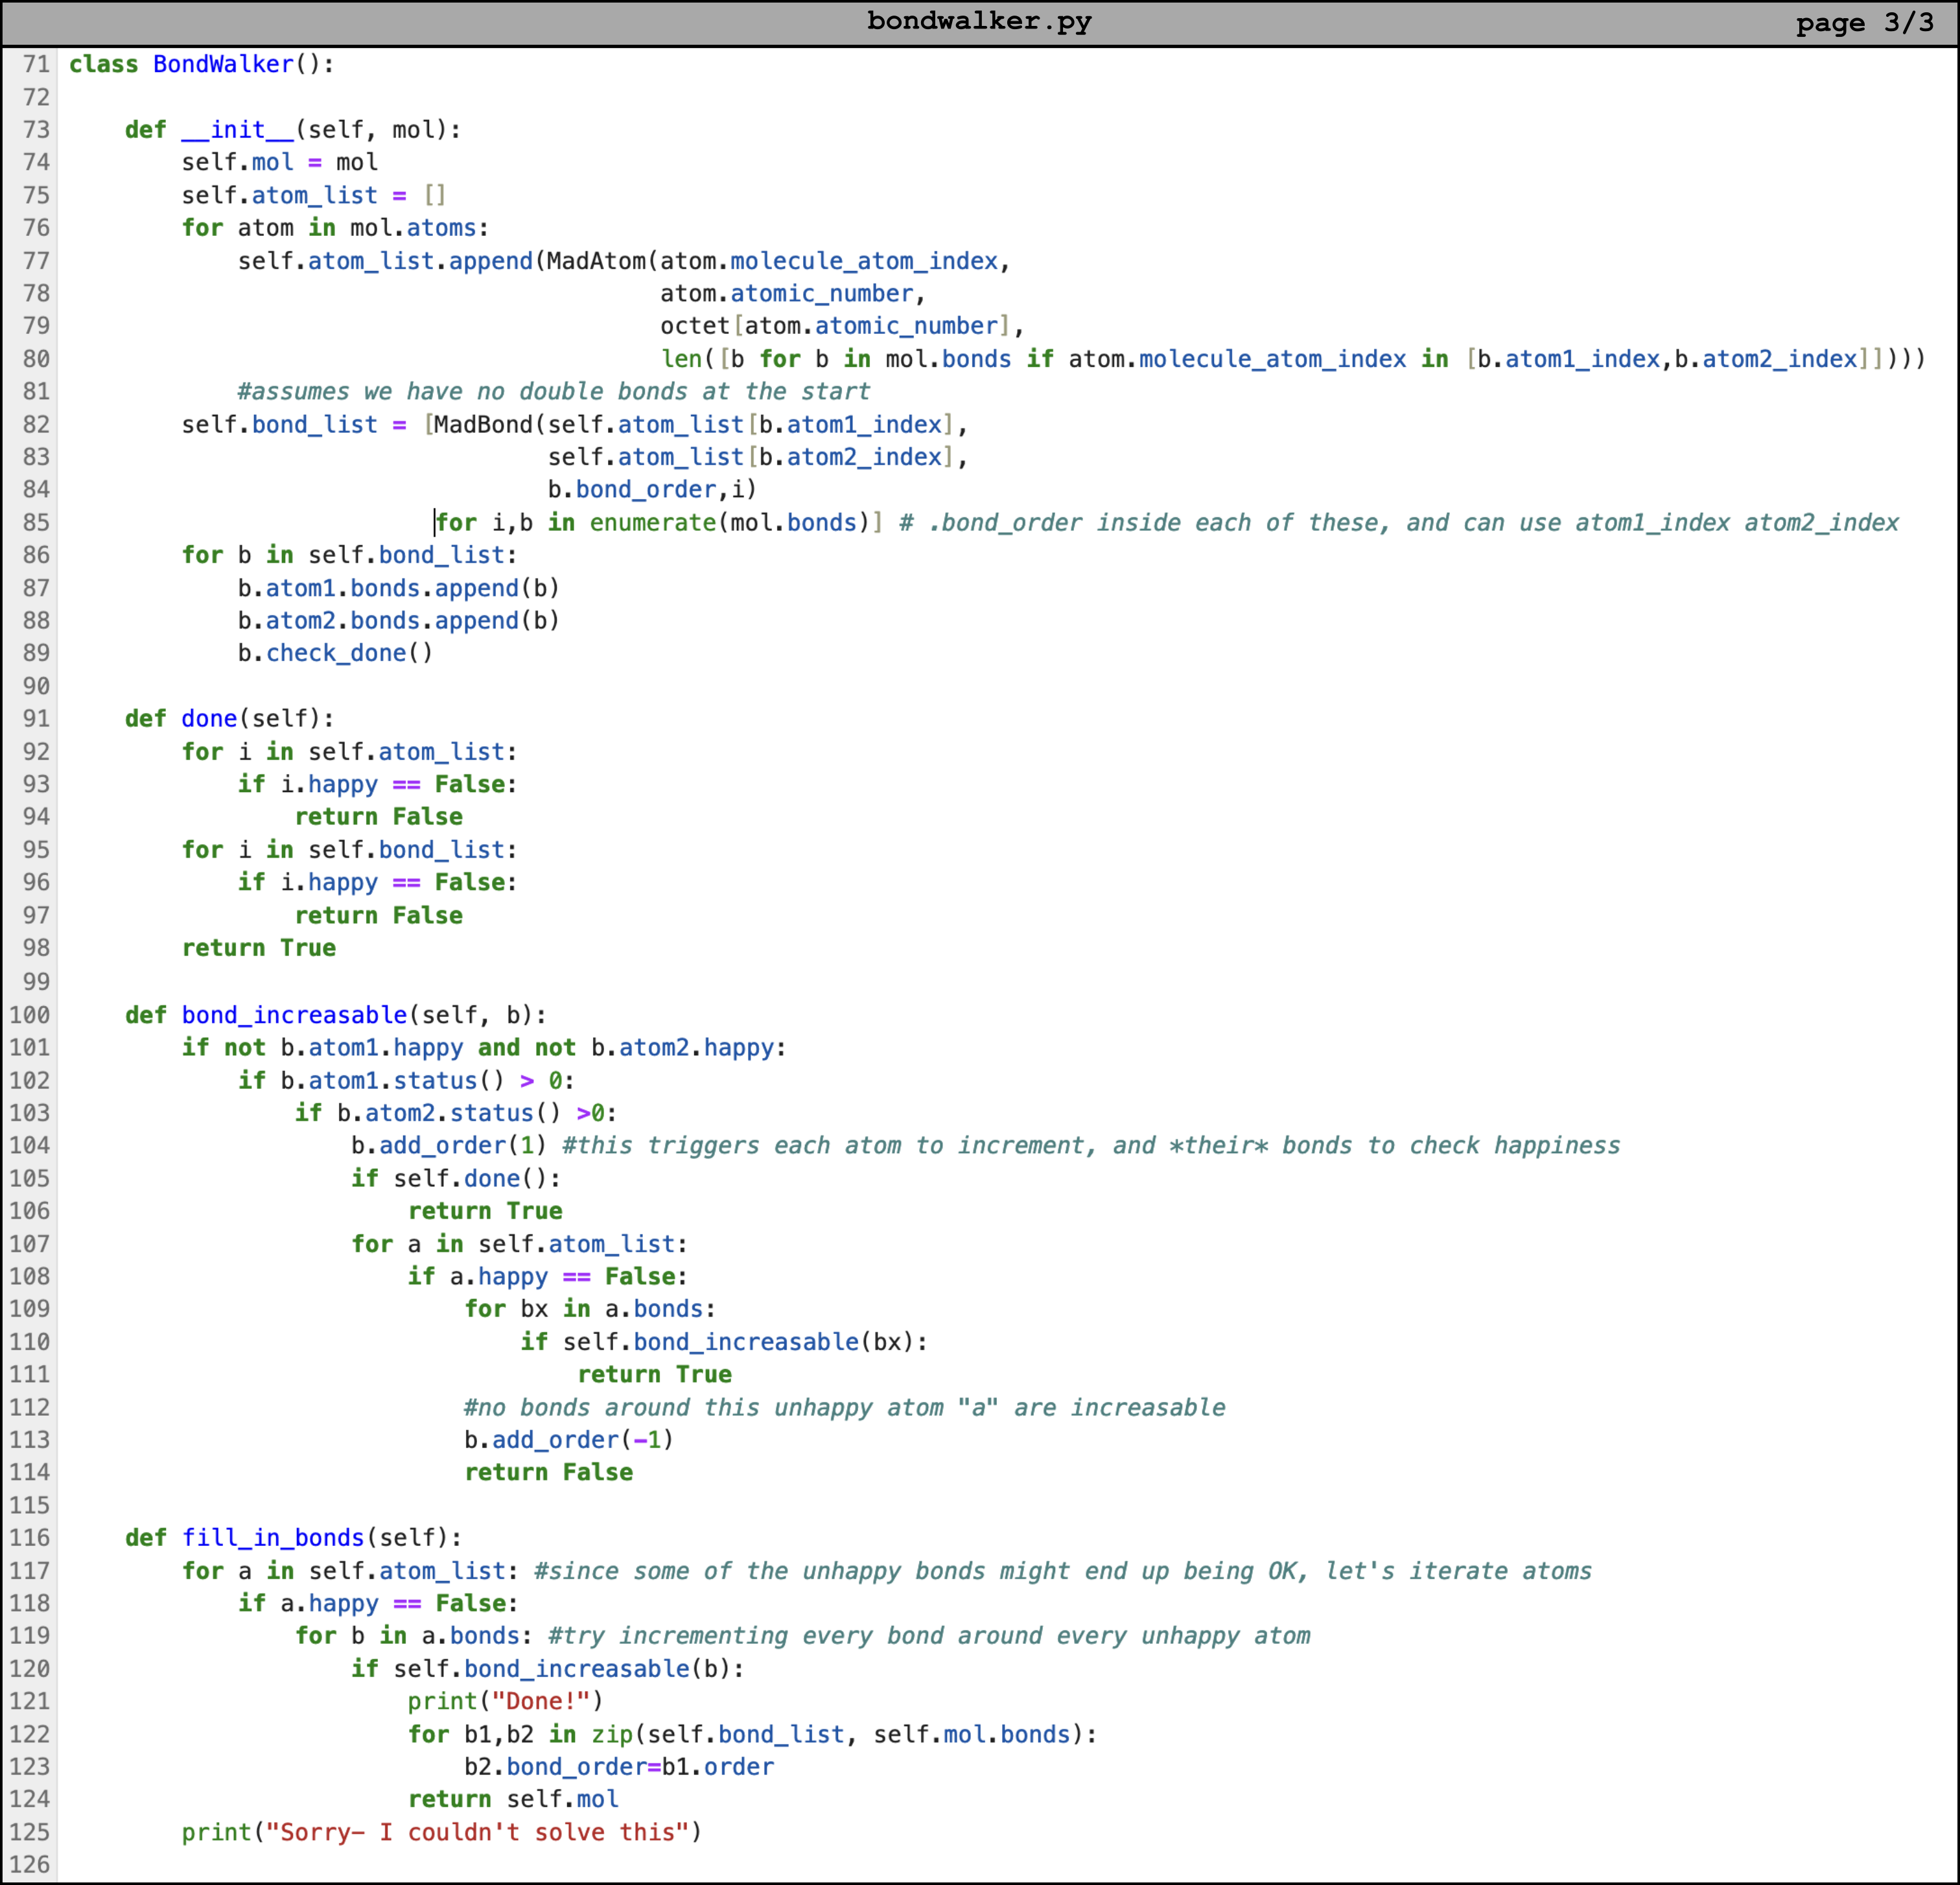
\includegraphics[width=1\linewidth]{src/figures/FF_figs/bw3.png}
    \label{fig:bw3}
\end{figure}


\chapter{Persistence Length Appendix}
\label{app:pers_len}

\begin{table}[ht]
    \centering
    \begin{tabular}{ll}

    \textbf{Polymer}  &     \textbf{Density} \\
    \hline
    PCPDTFBT-C1-BO    &     0.05    \\
    PCPDTFBT-C3-BO    &     0.05    \\
    PCPDTFBT-C4-BO    &     0.01    \\
    PCPDTFBT-C5-BO    &     0.05    \\
    PCPDTFBT-C11-BO   &     0.005   \\ 
    PCPDTPT-ene-HD    &     0.005   \\
    PCPDTPT-ene-ODD   &     0.05    \\
    PCPDTPT-HD        &     0.05    \\
    PCPDTPT-nC16      &     0.05    \\
    PCPDTPT-ODD       &     0.05    \\
    PIDTBT-nC16       &     0.05    \\
    PIDTCPDT-C11-BO   &     0.05    \\
    PIDTFBT-C11-BO    &     0.005   \\
    \end{tabular}
    \caption{Densities at which each polymer simulation was run at. All densities reported in units of g/mL}
    \label{densities}
\end{table}

\begin{table}[ht]
    \centering
    \begin{tabular}{l|l}
        \textbf{Polymer} & \textbf{TPS} \\
        \hline
        \textbf{PCPDTFBT-C11-BO  }   &       1027.1953   \\
        \textbf{PCPDTFBT-C1-BO   }    &       1085.1254   \\
        \textbf{PCPDTFBT-C3-BO   }   &       1134.8646   \\
        \textbf{PCPDTFBT-C4-BO   }   &       1021.8457   \\
        \textbf{PCPDTFBT-C5-BO   }   &       959.0328    \\
        \textbf{PCPDTPT-ene-HD   }    &       1987.0726   \\
        \textbf{PCPDTPT-ene-ODD  }    &       1717.0476   \\
        \textbf{PCPDTPT-HD       }   &       1443.4256   \\
        \textbf{PCPDTPT-nC16     }   &       1481.9449   \\
        \textbf{PCPDTPT-ODD      }   &       1425.6319   \\
        \textbf{PIDTBT-nC16      }   &       1025.8267   \\
        \textbf{PIDTCPDT-C11-BO  }   &       646.3932    \\
        \textbf{PIDTFBT-C11-BO   }   &       421.9683    \\
    \end{tabular}
    \caption{Average timesteps per second (TPS) for each polymer simulation. Values averaged over each simulation with temperatures ranging from 252 K to 2013 K.}
    \label{tab:pl_tps}
\end{table}

\begin{table}[ht]
    \centering
    \begin{tabular}{c|c|c|c|c}
                        &  \multicolumn{4}{c}{\textbf{l\textsubscript{p}}}  \\
        \hline
        \textbf{Polymer}  & \textbf{252 K} & \textbf{503 K} & \textbf{1006 K} & \textbf{SANS}\\
        \hline
        PCPDTFBT-C1-BO    &   $37.8 \pm 0.1$    &	$115.3 \pm 0.5$   &   $99.7 \pm 5.9$     &    67	 \\
        PCPDTFBT-C3-BO    &   $47.5 \pm 0.1$    &	$57.6 \pm 0.8$    &   $98.9 \pm 6.1$     &    78.4   \\
        PCPDTFBT-C4-BO    &   $46.3 \pm 0.3$    &	$65.8 \pm 0.9$    &   $105.1 \pm 5.6$    &    86.4   \\
        PCPDTFBT-C5-BO    &   $35.4 \pm 0.1$    &	$68.7\pm 0.5$     &   $104.3 \pm 7.8$    &    114	 \\
        PCPDTFBT-C11-BO   &   $34.6 \pm 0.1$    &	$55.9 \pm 0.7$    &   $104.0 \pm 7.4$    &    291	 \\
        PCPDTPT-ene-HD    &   $39.8 \pm 0.4$    &	$48.4 \pm 0.3$    &   $110.7 \pm 7.9$    &    76.6   \\
        PCPDTPT-ene-ODD   &   $21.9 \pm 0.1$    &	$38.5 \pm 0.3$    &   $97.8 \pm 7.3$     &    83.4   \\
        PCPDTPT-HD        &   $36.8 \pm 0.1$    &	$55.3 \pm 2.6$    &   $100.4 \pm 6.3$    &    47.3   \\
        PCPDTPT-nC16      &   $40.2 \pm 0.2$    &	$60.3 \pm 0.4$    &   $96.0 \pm 6.3$     &    61     \\
        PCPDTPT-ODD       &   $56.4 \pm 0.3$    &	$63.6 \pm 0.7$    &   $99.6 \pm 9.6$     &    54.9   \\
        PIDTBT-nC16       &   $65.4\pm 0.2$     &	$57.8 \pm 0.4$    &   $200.6 \pm 25.5$   &    1310   \\
        PIDTCPDT-C11-BO   &   $36.0 \pm 0.1$    &	$76.4 \pm 2.4$    &   $182.2 \pm 13.7$   &    236	 \\
        PIDTFBT-C11-BO    &   $79.4 \pm 1.1$    &	$90.6 \pm 6.5$    &   $178.4 \pm 9.2$    &    254	 \\
    \end{tabular}
    \caption{Caption}
    \label{tab:l_p}
\end{table}

\begin{table}[ht]
    \centering
    \begin{tabular}{c|c}
    \textbf{Polymer}   &    \textbf{$T_{SANS}$}\\
    \hline
    PCPDTFBT-C1-BO     &    326\\
    PCPDTFBT-C3-BO     &    736\\
    PCPDTFBT-C4-BO     &    767\\
    PCPDTFBT-C5-BO     &    1091\\
    PCPDTFBT-C11-BO    &    3035\\
    PCPDTPT-ene-HD     &    692\\
    PCPDTPT-ene-ODD    &    885\\
    PCPDTPT-HD         &    389\\
    PCPDTPT-nC16       &    526\\
    PCPDTPT-ODD        &    278\\
    PIDTBT-nC16        &    6785\\
    PIDTCPDT-C11-BO    &    1290\\
    PIDTFBT-C11-BO     &    1591\\
    \end{tabular}
    \caption{Predicted simulation temperature at which $l_p^{MD}$ would match $l_p^{SANS}$.}
    \label{tab:T_sans}
\end{table}

\newpage % NOTE: The appendix title should be on its own page.

\begin{figure}
    \centering
    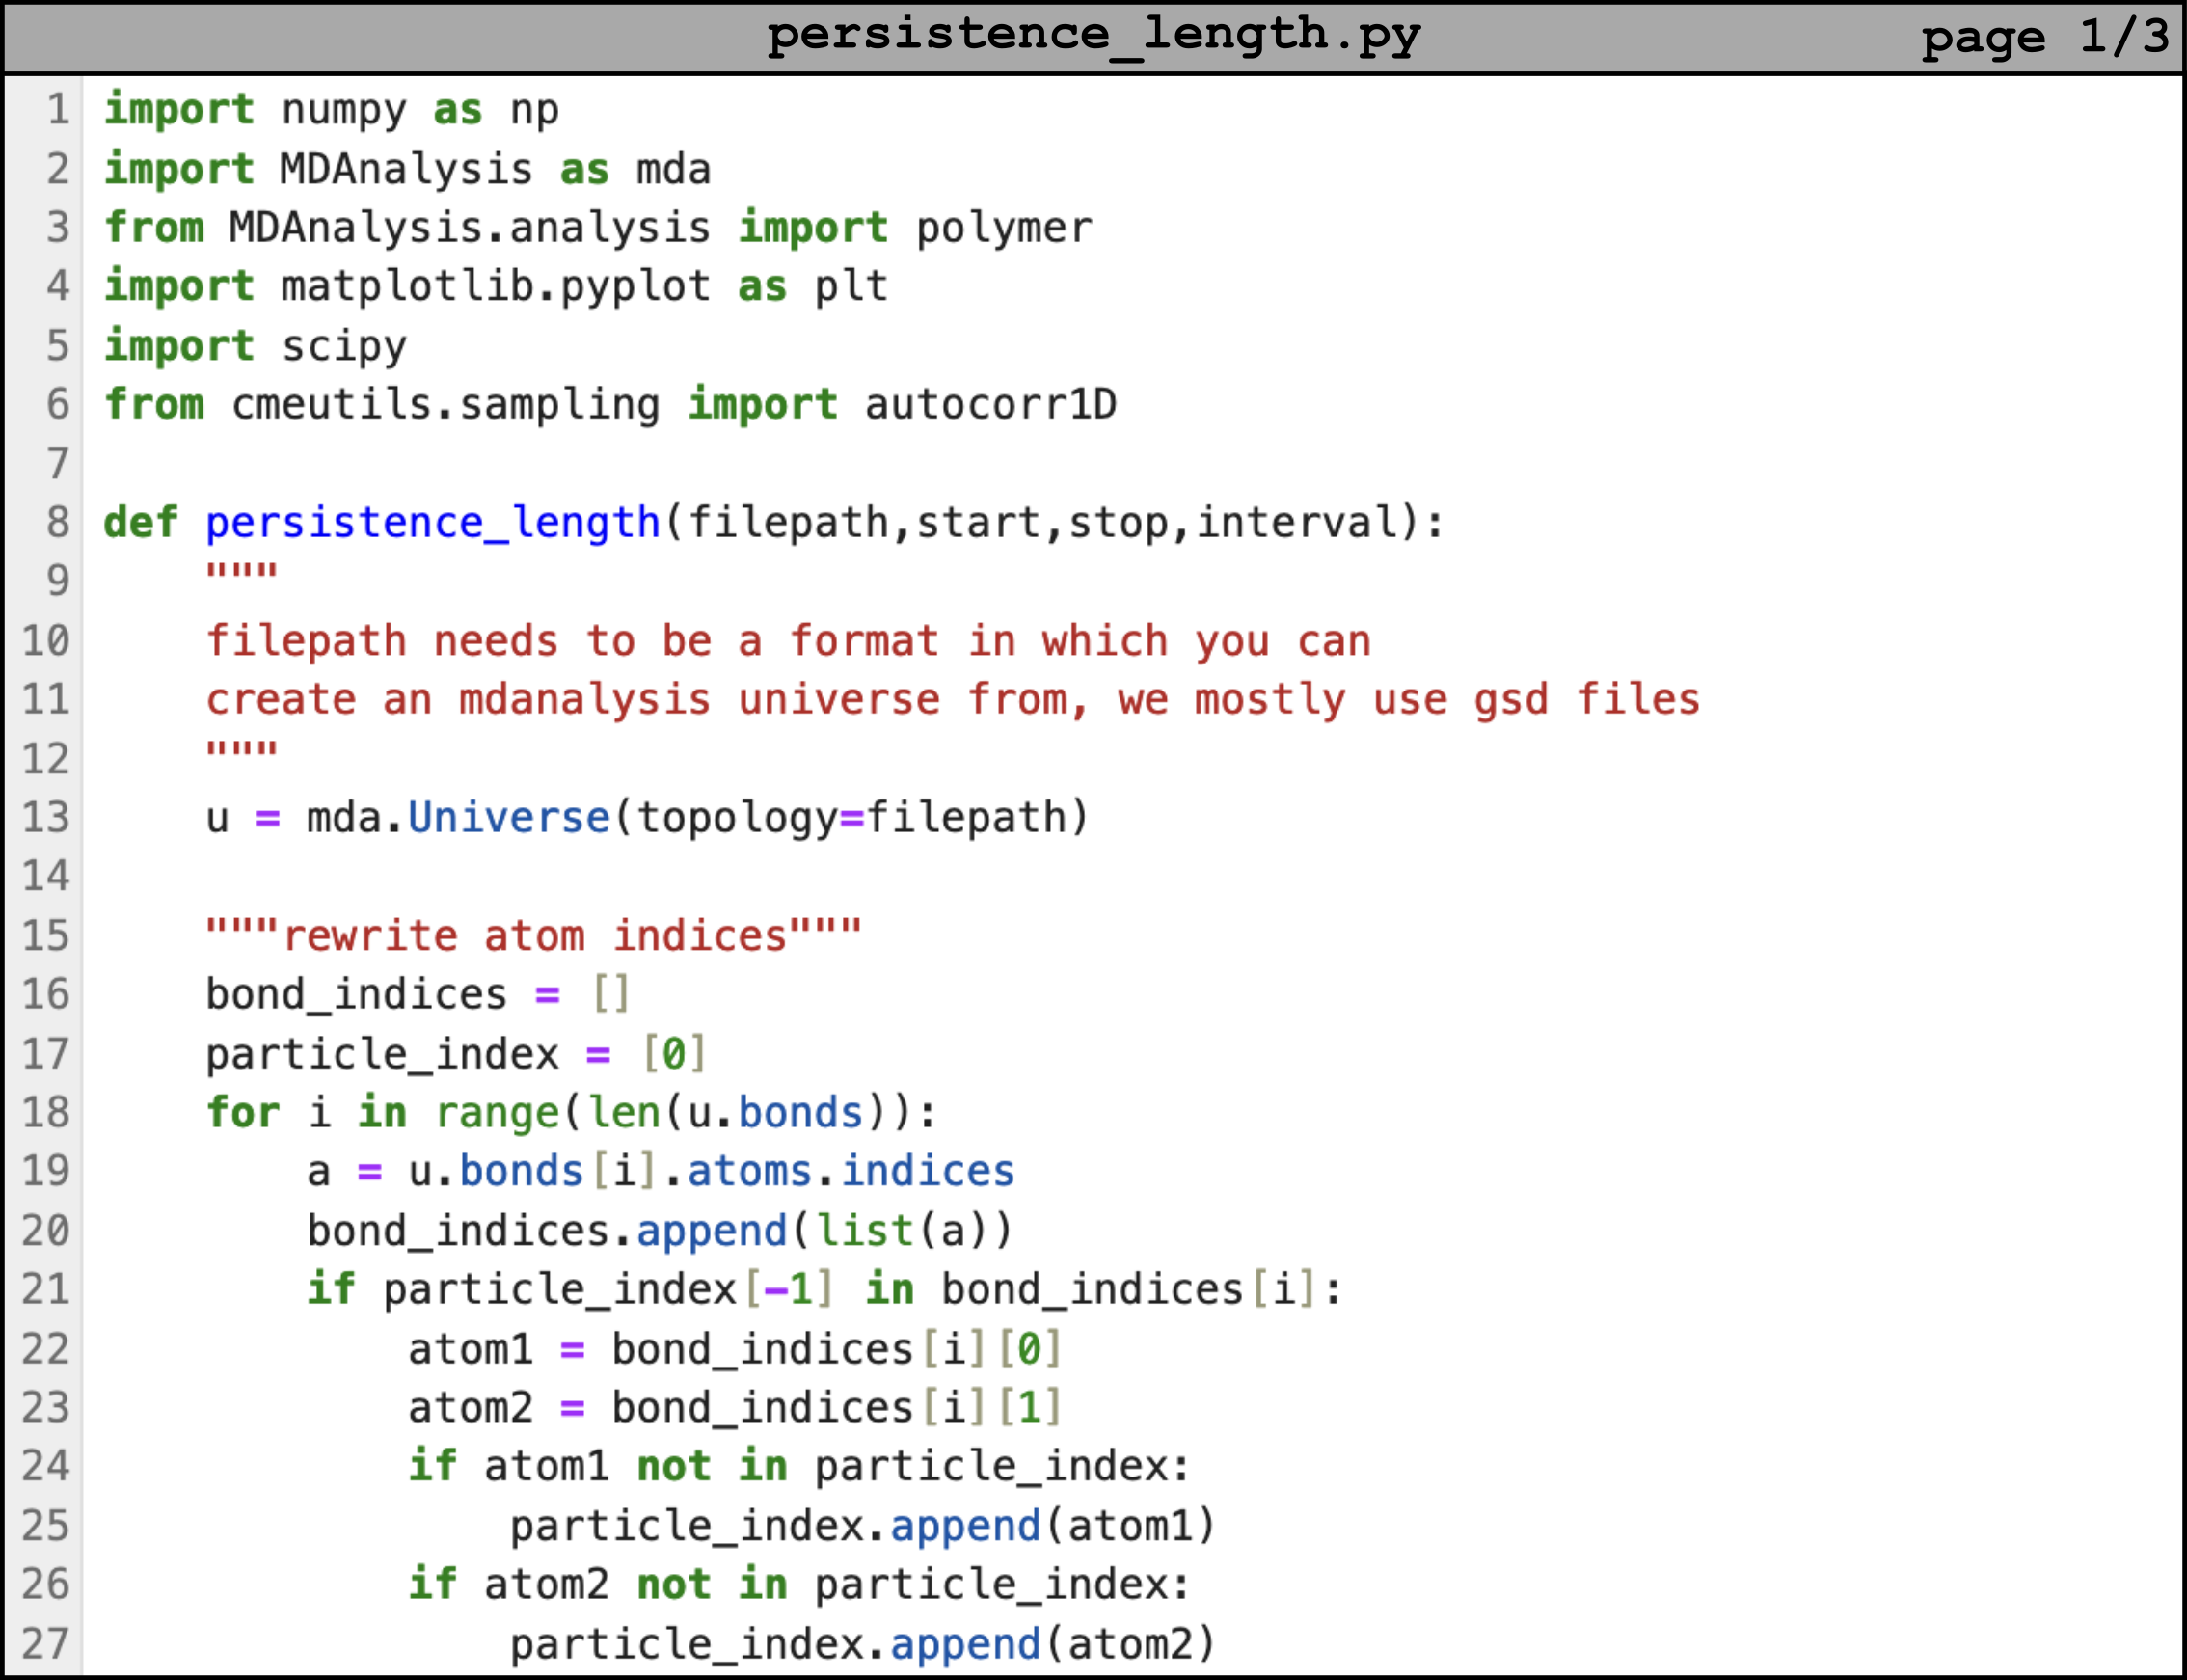
\includegraphics[width=1\linewidth]{src/figures/pers_l_figs/pers_len1.png}
    \label{fig:pers_len1}
\end{figure}

\newpage 

\begin{figure}
    \centering
    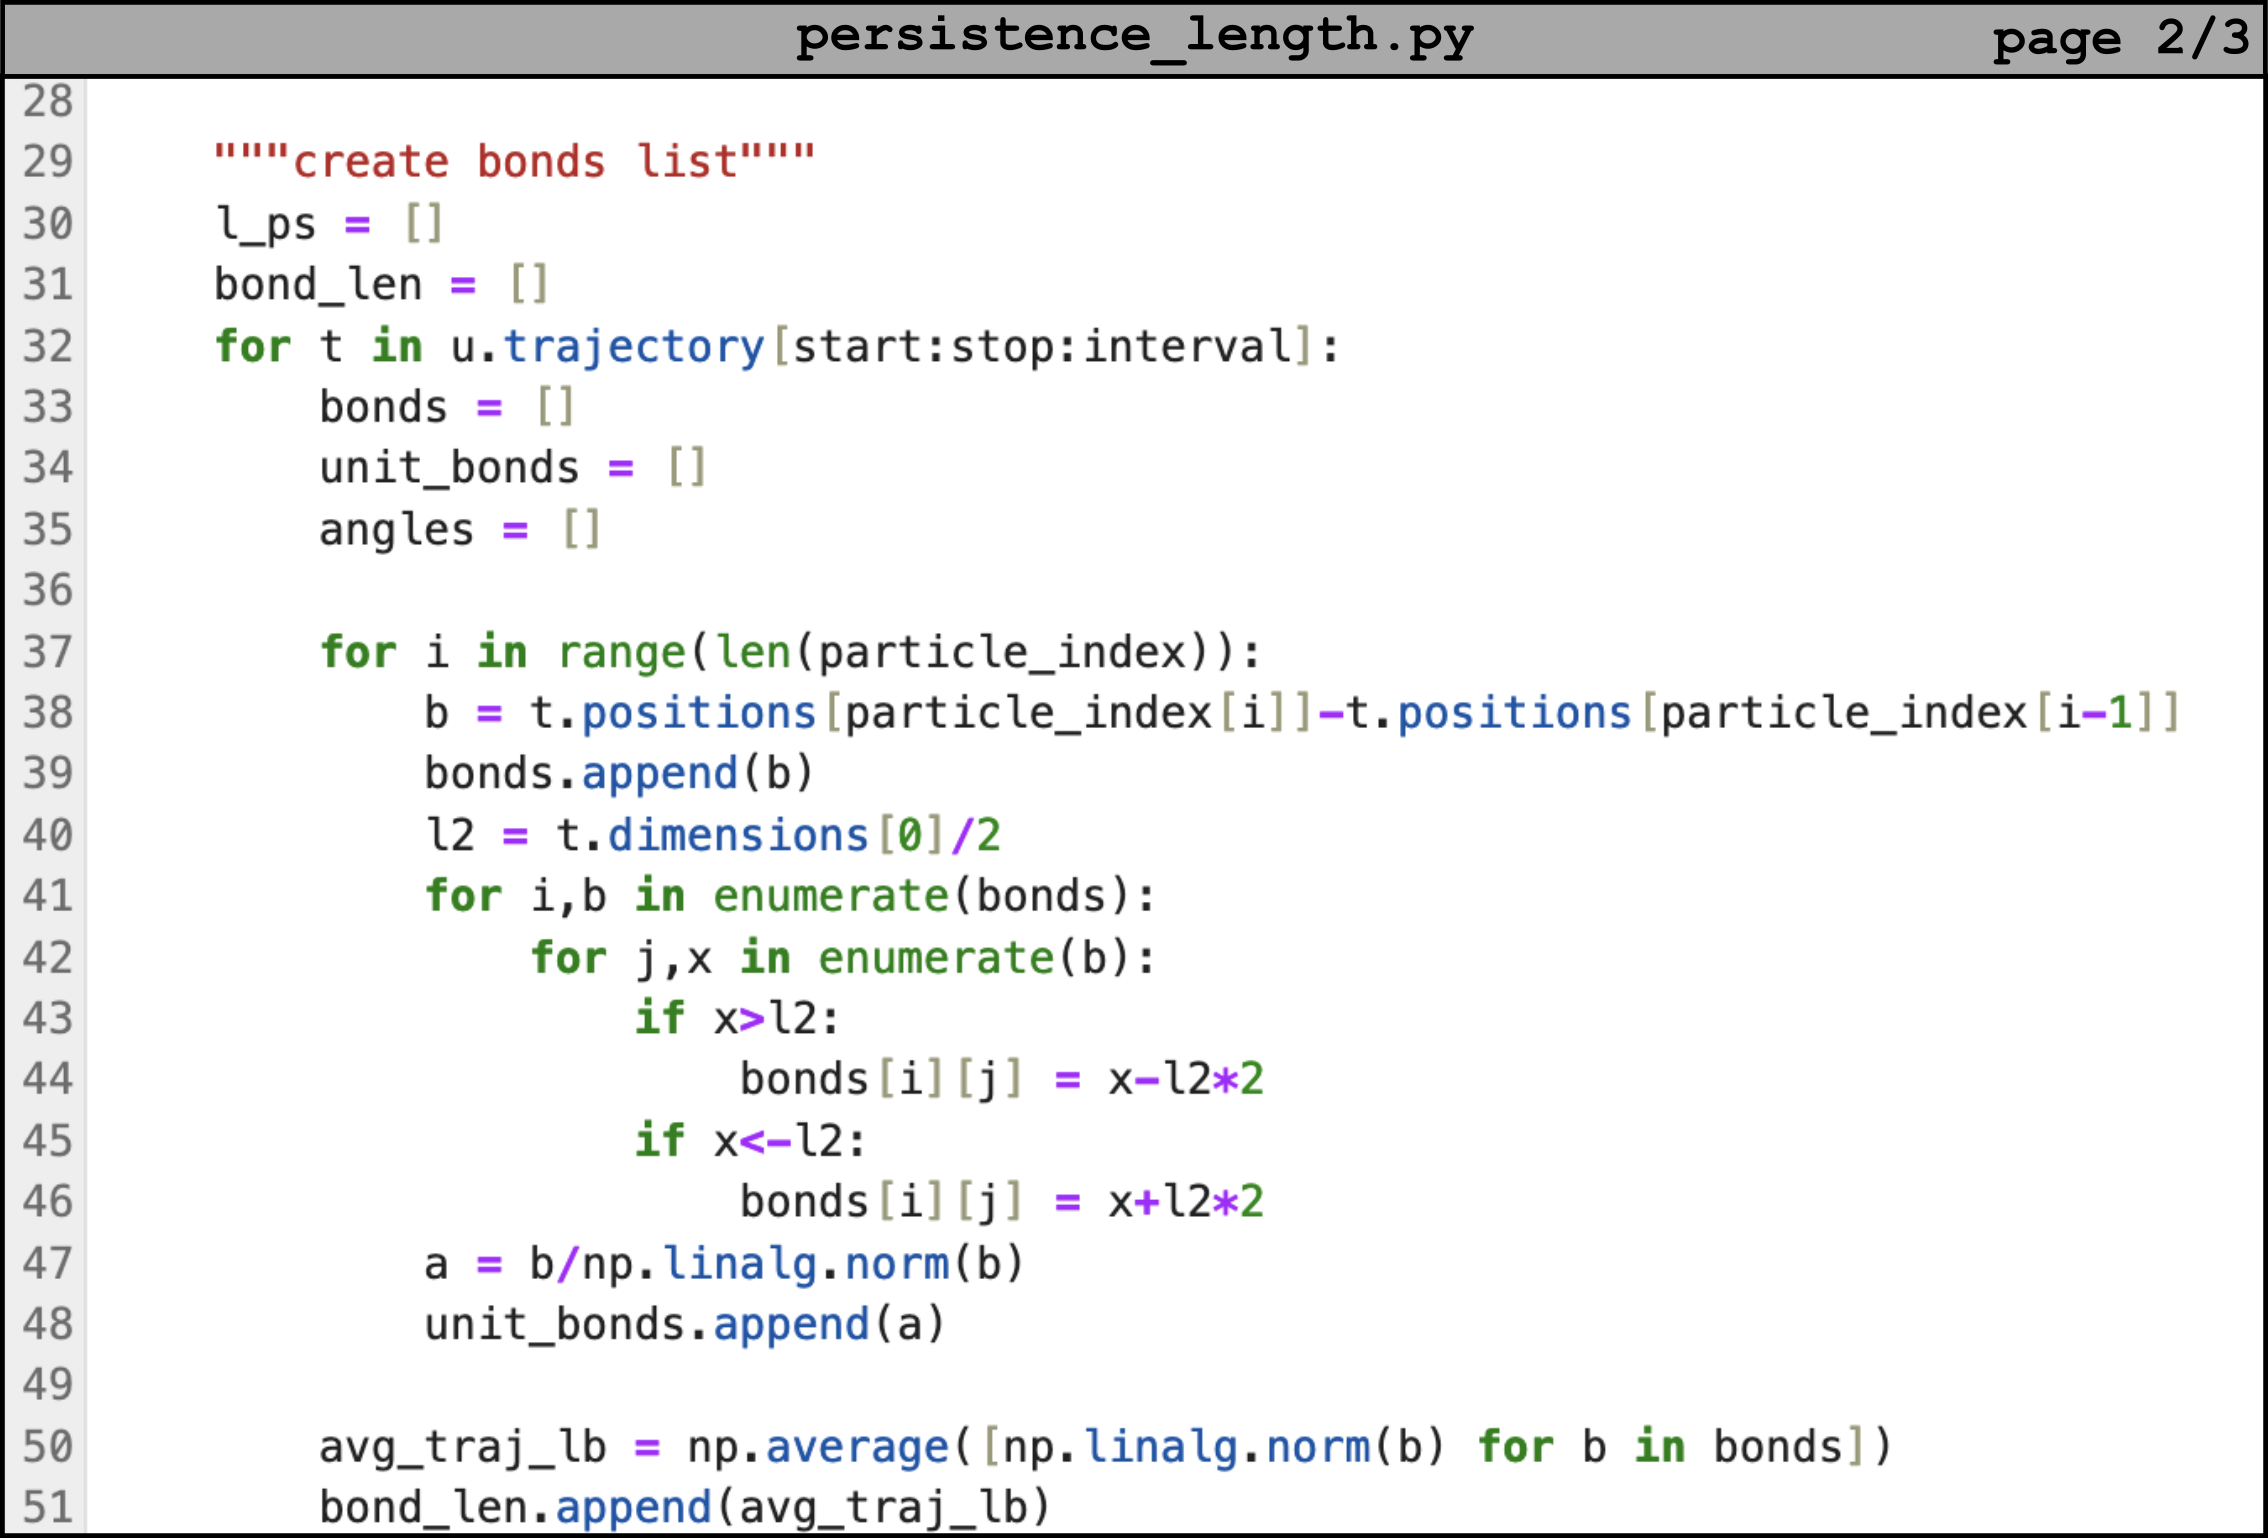
\includegraphics[width=1\linewidth]{src/figures/pers_l_figs/pers_len2.png}
    \label{fig:pers_len2}
\end{figure}

\newpage 

\begin{figure}
    \centering
    \includegraphics[width=1\linewidth]{src/figures/pers_l_figs/pers_len3.png}
    \label{fig:pers_len3}
\end{figure}

\clearpage

\begin{figure}
    \centering
    \includegraphics[width=1\linewidth]{src/figures/pers_l_figs/real_cond_polymer.png}
    \caption{Snapshot of coarse grained PCPDTPT-HD at a temperature of 252 K and density of 0.05 g/mol. The red highlighted CG beads have parallel aligned bond vectors. The blue highlighted CG beads are parallel, but anti-aligned with the red.}
    \label{fig:real_cond_polymer}
\end{figure}


\begin{figure}
    \centering
    \includegraphics[width=1\linewidth]{src/figures/pers_l_figs/untitled folder/pcpdtpt/eneHD_plot.jpeg}
    \caption{Persistence length ($l_p^{MD}$) of PCPDTPT-eneHD vs Temperature plot with a linear regression calculated using SciPy \citep{2020SciPy-NMeth} and $T_{SANS}$ prediction.}
    \label{fig:eneHD_plot}
\end{figure}

\begin{figure}
    \centering
    \includegraphics[width=1\linewidth]{src/figures/pers_l_figs/untitled folder/pcpdtpt/eneODD_plot.jpeg}
    \caption{Persistence length ($l_p^{MD}$) of PCPDTPT-eneODD vs Temperature plot with a linear regression calculated using SciPy \citep{2020SciPy-NMeth} and $T_{SANS}$ prediction.}
    \label{fig:eneODD_plot}
\end{figure}

\begin{figure}
    \centering
    \includegraphics[width=1\linewidth]{src/figures/pers_l_figs/untitled folder/pcpdtpt/HD_plot.jpeg}
    \caption{Persistence length ($l_p^{MD}$) of PCPDTPT-HD vs Temperature plot with a linear regression calculated using SciPy \citep{2020SciPy-NMeth} and $T_{SANS}$ prediction.}
    \label{fig:HD_plot}
\end{figure}

\begin{figure}
    \centering
    \includegraphics[width=1\linewidth]{src/figures/pers_l_figs/untitled folder/pcpdtpt/ODD_plot.jpeg}
    \caption{Persistence length ($l_p^{MD}$) of PCPDTPT-ODD vs Temperature plot with a linear regression calculated using SciPy \citep{2020SciPy-NMeth} and $T_{SANS}$ prediction.}
    \label{fig:ODD_plot}
\end{figure}

\begin{figure}
    \centering
    \includegraphics[width=1\linewidth]{src/figures/pers_l_figs/untitled folder/pcpdtpt/nC16_plot.jpeg}
    \caption{Persistence length ($l_p^{MD}$) of PCPDTPT-nC16 vs Temperature plot with a linear regression calculated using SciPy \citep{2020SciPy-NMeth} and $T_{SANS}$ prediction.}
    \label{fig:nC16_plot}
\end{figure}


\begin{figure}
    \centering
    \includegraphics[width=1\linewidth]{src/figures/pers_l_figs/untitled folder/pcpdtfbt/C1_plot.jpeg}
    \caption{Persistence length ($l_p^{MD}$) of PCPDTFBT-C1-BO vs Temperature plot with a linear regression calculated using SciPy \citep{2020SciPy-NMeth} and $T_{SANS}$ prediction.}
    \label{fig:C1_plot}
\end{figure}

\begin{figure}
    \centering
    \includegraphics[width=1\linewidth]{src/figures/pers_l_figs/untitled folder/pcpdtfbt/C3_plot.jpeg}
    \caption{Persistence length ($l_p^{MD}$) of PCPDTFBT-C3-BO vs Temperature plot with a linear regression calculated using SciPy \citep{2020SciPy-NMeth} and $T_{SANS}$ prediction.}
    \label{fig:C3_plot}
\end{figure}

\begin{figure}
    \centering
    \includegraphics[width=1\linewidth]{src/figures/pers_l_figs/untitled folder/pcpdtfbt/c4_plot.jpeg}
    \caption{Persistence length ($l_p^{MD}$) of PCPDTFBT-C4-BO vs Temperature plot with a linear regression calculated using SciPy \citep{2020SciPy-NMeth} and $T_{SANS}$ prediction.}
    \label{fig:C4_plot}
\end{figure}

\begin{figure}
    \centering
    \includegraphics[width=1\linewidth]{src/figures/pers_l_figs/untitled folder/pcpdtfbt/C5_plot.jpeg}
    \caption{Persistence length ($l_p^{MD}$) of PCPDTFBT-C5-BO vs Temperature plot with a linear regression calculated using SciPy \citep{2020SciPy-NMeth} and $T_{SANS}$ prediction.}
    \label{fig:C5_plot}
\end{figure}

\begin{figure}
    \centering
    \includegraphics[width=1\linewidth]{src/figures/pers_l_figs/untitled folder/pcpdtfbt/C11_plot.jpeg}
    \caption{Persistence length ($l_p^{MD}$) of PCPDTFBT-C11-BO vs Temperature plot with a linear regression calculated using SciPy \citep{2020SciPy-NMeth} and $T_{SANS}$ prediction.}
    \label{fig:C11_plot}
\end{figure}


\begin{figure}
    \centering
    \includegraphics[width=1\linewidth]{src/figures/pers_l_figs/untitled folder/idt/nc16_plot.jpeg}
    \caption{Persistence length ($l_p^{MD}$) of PIDTBT-nC16 vs Temperature plot with a linear regression calculated using SciPy \citep{2020SciPy-NMeth} and $T_{SANS}$ prediction.}
    \label{fig:idtnc16_plot}
\end{figure}

\begin{figure}
    \centering
    \includegraphics[width=1\linewidth]{src/figures/pers_l_figs/untitled folder/idt/cpdt_plot.jpeg}
    \caption{Persistence length ($l_p^{MD}$) of PIDTCPDT-C11-BO vs Temperature plot with a linear regression calculated using SciPy \citep{2020SciPy-NMeth} and $T_{SANS}$ prediction.}
    \label{fig:idtcpdt_plot}
\end{figure}

\begin{figure}
    \centering
    \includegraphics[width=1\linewidth]{src/figures/pers_l_figs/untitled folder/idt/fbt_plot.jpeg}
    \caption{Persistence length ($l_p^{MD}$) of PIDTFBT-C11-BO vs Temperature plot with a linear regression calculated using SciPy \citep{2020SciPy-NMeth} and $T_{SANS}$ prediction.}
    \label{fig:idt_fbt_plot}
\end{figure}


\begin{figure}
    \centering
    \includegraphics[width=0.6\linewidth]{src/figures/pers_l_figs/e-e plots/C1.png}
    \caption{$\sqrt{\langle R^2 \rangle}$ vs Temperature for PCPDTFBT-C1-BO with a linear regression for the linear portion of the plot. Horizontal line plotted at $\sqrt{N_b}*l_b$.}
    \label{fig:e-e_C1}
\end{figure}

\begin{figure}
    \centering
    \includegraphics[width=0.6\linewidth]{src/figures/pers_l_figs/e-e plots/C3.png}
    \caption{$\sqrt{\langle R^2 \rangle}$ vs Temperature for PCPDTFBT-C3-BO with a linear regression for the linear portion of the plot. Horizontal line plotted at $\sqrt{N_b}*l_b$.}
    \label{fig:e-e_C3}
\end{figure}

\begin{figure}
    \centering
    \includegraphics[width=0.6\linewidth]{src/figures/pers_l_figs/e-e plots/C4.png}
    \caption{$\sqrt{\langle R^2 \rangle}$ vs Temperature for PCPDTFBT-C4-BO with a linear regression for the linear portion of the plot. Horizontal line plotted at $\sqrt{N_b}*l_b$.}
    \label{fig:e-e_C4}
\end{figure}

\begin{figure}
    \centering
    \includegraphics[width=0.6\linewidth]{src/figures/pers_l_figs/e-e plots/C5.png}
    \caption{$\sqrt{\langle R^2 \rangle}$ vs Temperature for PCPDTFBT-C5-BO with a linear regression for the linear portion of the plot. Horizontal line plotted at $\sqrt{N_b}*l_b$.}
    \label{fig:e-e_C5}
\end{figure}

\begin{figure}
    \centering
    \includegraphics[width=0.6\linewidth]{src/figures/pers_l_figs/e-e plots/C11.png}
    \caption{$\sqrt{\langle R^2 \rangle}$ vs Temperature for PCPDTFBT-C11-BO with a linear regression for the linear portion of the plot. Horizontal line plotted at $\sqrt{N_b}*l_b$.}
    \label{fig:e-e_C11}
\end{figure}

\begin{figure}
    \centering
    \includegraphics[width=0.6\linewidth]{src/figures/pers_l_figs/e-e plots/ene_HD.png}
    \caption{$\sqrt{\langle R^2 \rangle}$ vs Temperature for PCPDTPT-ene-HD with a linear regression for the linear portion of the plot. Horizontal line plotted at $\sqrt{N_b}*l_b$.}
    \label{fig:e-e_ene_HD}
\end{figure}

\begin{figure}
    \centering
    \includegraphics[width=0.6\linewidth]{src/figures/pers_l_figs/e-e plots/ene_ODD.png}
    \caption{$\sqrt{\langle R^2 \rangle}$ vs Temperature for PCPDTPT-ene-ODD with a linear regression for the linear portion of the plot. Horizontal line plotted at $\sqrt{N_b}*l_b$.}
    \label{fig:e-e_ene_ODD}
\end{figure}

\begin{figure}
    \centering
    \includegraphics[width=0.6\linewidth]{src/figures/pers_l_figs/e-e plots/HD.png}
    \caption{$\sqrt{\langle R^2 \rangle}$ vs Temperature for PCPDTPT-HD with a linear regression for the linear portion of the plot. Horizontal line plotted at $\sqrt{N_b}*l_b$.}
    \label{fig:e-e_HD}
\end{figure}

\begin{figure}
    \centering
    \includegraphics[width=0.6\linewidth]{src/figures/pers_l_figs/e-e plots/nC16.png}
    \caption{$\sqrt{\langle R^2 \rangle}$ vs Temperature for PCPDTPT-nC16 with a linear regression for the linear portion of the plot. Horizontal line plotted at $\sqrt{N_b}*l_b$.}
    \label{fig:e-e_nC16}
\end{figure}

\begin{figure}
    \centering
    \includegraphics[width=0.6\linewidth]{src/figures/pers_l_figs/e-e plots/ODD.png}
    \caption{$\sqrt{\langle R^2 \rangle}$ vs Temperature for PCPDTPT-ODD with a linear regression for the linear portion of the plot. Horizontal line plotted at $\sqrt{N_b}*l_b$.}
    \label{fig:e-e_ODD}
\end{figure}

\begin{figure}
    \centering
    \includegraphics[width=0.6\linewidth]{src/figures/pers_l_figs/e-e plots/PIDT_nC16.png}
    \caption{$\sqrt{\langle R^2 \rangle}$ vs Temperature for PIDTBT-nC16 with a linear regression for the linear portion of the plot. Horizontal line plotted at $\sqrt{N_b}*l_b$.}
    \label{fig:e-e_PIDTBT}
\end{figure}

\begin{figure}
    \centering
    \includegraphics[width=0.6\linewidth]{src/figures/pers_l_figs/e-e plots/PIDT_CPDT.png}
    \caption{$\sqrt{\langle R^2 \rangle}$ vs Temperature for PIDTCPDT-C11-BO with a linear regression for the linear portion of the plot. Horizontal line plotted at $\sqrt{N_b}*l_b$.}
    \label{fig:e-e_PIDTCPDT}
\end{figure}

\begin{figure}
    \centering
    \includegraphics[width=0.6\linewidth]{src/figures/pers_l_figs/e-e plots/PIDT_FBT.png}
    \caption{$\sqrt{\langle R^2 \rangle}$ vs Temperature for PIDTBFT-C11-BO with a linear regression for the linear portion of the plot. Horizontal line plotted at $\sqrt{N_b}*l_b$.}
    \label{fig:e-e_FBT}
\end{figure}
%------------------------------------------------------------------------------

\end{document}